%%%%%%%%%%%%%%%%%%%%%%%%%%%%%%%%%%%%%%%%%
% Masters Thesis
% LaTeX Template
%
% This template is based on a template by:
% Steve Gunn (http://users.ecs.soton.ac.uk/srg/softwaretools/document/templates/)
% Sunil Patel (http://www.sunilpatel.co.uk/thesis-template/)
%
% Template license:
% CC BY-NC-SA 3.0 (http://creativecommons.org/licenses/by-nc-sa/3.0/)
%
%%%%%%%%%%%%%%%%%%%%%%%%%%%%%%%%%%%%%%%%%

%----------------------------------------------------------------------------------------
%	PACKAGES AND OTHER DOCUMENT CONFIGURATIONS
%----------------------------------------------------------------------------------------

\documentclass[
11pt, % The default document font size, options: 10pt, 11pt, 12pt
%oneside, % Two side (alternating margins) for binding by default, uncomment to switch to one side
english, % ngerman for German
onehalfspacing, % Single line spacing, alternatives: onehalfspacing or doublespacing
%draft, % Uncomment to enable draft mode (no pictures, no links, overfull hboxes indicated)
%nolistspacing, % If the document is onehalfspacing or doublespacing, uncomment this to set spacing in lists to single
%liststotoc, % Uncomment to add the list of figures/tables/etc to the table of contents
%toctotoc, % Uncomment to add the main table of contents to the table of contents
%parskip, % Uncomment to add space between paragraphs
%nohyperref, % Uncomment to not load the hyperref package
headsepline, % Uncomment to get a line under the header
%chapterinoneline, % Uncomment to place the chapter title next to the number on one line
%consistentlayout, % Uncomment to change the layout of the declaration, abstract and acknowledgements pages to match the default layout
]{MastersDoctoralThesis} % The class file specifying the document structure

\usepackage[utf8]{inputenc} % Required for inputting international characters
\usepackage[T1]{fontenc} % Output font encoding for international characters

\usepackage{mathpazo} % Use the Palatino font by default

\usepackage[backend=bibtex,style=authoryear,natbib=true]{biblatex} % Use the bibtex backend with the authoryear citation style (which resembles APA)

\addbibresource{references.bib}
\addbibresource{research/clustering_recent_references.bib} % The filename of the bibliography

% --- Citation style: square-bracket author-year with "et al." (match reference TFM) ---
\ExecuteBibliographyOptions{maxcitenames=2,mincitenames=1}
\renewcommand*{\nameyeardelim}{\addcomma\space} % renders as [Author, year]
\DeclareCiteCommand{\parencite}[\mkbibbrackets]
  {\usebibmacro{prenote}}
  {\usebibmacro{citeindex}\usebibmacro{cite}}
  {\multicitedelim}
  {\usebibmacro{postnote}}
\let\autocite\parencite
\let\textcite\parencite % bracket subject-citations too, as in the reference thesis

% --- Hyperlink colours (match reference TFM) ---
\definecolor{linkcol}{HTML}{1B7F79} % teal: internal cross-references
\definecolor{citecol}{HTML}{B5179E} % magenta: citations
\definecolor{urlcol}{HTML}{7B241C}  % maroon: URLs / DOIs

\usepackage[autostyle=true]{csquotes} % Required to generate language-dependent quotes in the bibliography

\usepackage{amsmath} % Mathematical symbols and environments
\usepackage{amssymb} % Additional math symbols (\mathbb, etc.)
\usepackage{booktabs} % Better table formatting
\usepackage{graphicx} % Enhanced graphics support
\usepackage{caption} % Better caption control
\usepackage{subcaption} % Sub-figures
\usepackage{tikz} % Pipeline diagram in Chapter 3

\emergencystretch=2em % Allow whitespace stretch to avoid overfull hboxes
\tolerance=1500 % Slightly more tolerant line breaking

%----------------------------------------------------------------------------------------
%	MARGIN SETTINGS
%----------------------------------------------------------------------------------------

\geometry{
	paper=a4paper, % Change to letterpaper for US letter
	inner=2.5cm, % Inner margin
	outer=3.8cm, % Outer margin
	bindingoffset=0.5cm, % Binding offset
	top=1.5cm, % Top margin
	bottom=1.5cm, % Bottom margin
	%showframe, % Uncomment to show how the type block is set on the page
}

%----------------------------------------------------------------------------------------
%	THESIS INFORMATION
%----------------------------------------------------------------------------------------

\thesistitle{Data-Driven Cognitive Phenotyping in Acquired Brain Injury: A Clustering Analysis with Imputation Robustness Assessment} % Your thesis title
\supervisor{Dr.\ Alejandro García-Rudolph} % Your supervisor's name
\examiner{} % Your examiner's name
\degree{MSc} % Your degree name
\author{Zoltan Kunos} % Your name
\addresses{} % Your address

\subject{Data Science} % Your subject area
\keywords{acquired brain injury, cognitive phenotyping, clustering, UMAP, HDBSCAN, missing data imputation, neuropsychology} % Keywords
\university{\href{http://www.ub.edu}{Universitat de Barcelona}} % Your university's name and URL, this is used in the title page and abstract, print it elsewhere with \univname
\department{} % No department URL supplied.
\group{} % Your research group's name and URL, this is used in the title page, print it elsewhere with \groupname
\faculty{\href{http://mat.ub.edu}{Facultat de Matemàtiques i Informàtica}} % Your faculty's name and URL, this is used in the title page and abstract, print it elsewhere with \facname

\AtBeginDocument{
\hypersetup{pdftitle=\ttitle} % Set the PDF's title to your title
\hypersetup{pdfauthor=\authorname} % Set the PDF's author to your name
\hypersetup{pdfkeywords=\keywordnames} % Set the PDF's keywords to your keywords
\hypersetup{linkcolor=linkcol} % Teal cross-references
\hypersetup{citecolor=citecol} % Magenta citations
\hypersetup{urlcolor=urlcol} % Maroon URLs / DOIs
}

\begin{document}

\frontmatter % Use roman page numbering style (i, ii, iii, iv...) for the pre-content pages

\pagestyle{plain} % Default to the plain heading style until the thesis style is called for the body content

%----------------------------------------------------------------------------------------
%	TITLE PAGE
%----------------------------------------------------------------------------------------

\begin{titlepage}
\begin{center}

\vspace*{0.06\textheight}
{\scshape\LARGE \univname\par}\vspace{1.5cm} % University name
\textsc{\Large Fundamental Principles of Data Science Master's Thesis}\\[0.5cm] % Thesis type

\HRule \\[0.4cm] % Horizontal line
{\huge \bfseries \ttitle\par}\vspace{0.4cm} % Thesis title
\HRule \\[1.5cm] % Horizontal line

\begin{minipage}[t]{0.4\textwidth}
\begin{flushleft} \large
\emph{Author:}\\
\authorname
\end{flushleft}
\end{minipage}
\begin{minipage}[t]{0.4\textwidth}
\begin{flushright} \large
\emph{Supervisor:} \\
\supname
\end{flushright}
\end{minipage}\\[3cm]

\vfill

\large \textit{A thesis submitted in partial fulfillment of the requirements\\ for the degree of MSc in Fundamental Principles of Data Science}\\[0.3cm] % University requirement text
\textit{in the}\\[0.4cm]
\facname\\[2cm] % Research group name and department name

\vfill

{\large \today}\\[4cm] % Date
%\includegraphics{Logo} % University/department logo - uncomment to place it

\vfill
\end{center}
\end{titlepage}


%----------------------------------------------------------------------------------------
%	ABSTRACT PAGE
%----------------------------------------------------------------------------------------

\begin{abstract}[]
\addchaptertocentry{\abstractname}
Neuropsychological evaluations of people who have experienced an acquired brain injury (ABI) are often incomplete. This research addressed this by exploring whether the use of "clustering" would allow for a consistent representation of cognitive function despite two challenges: What method(s) would be used to replace missing information from the evaluation? How could the characteristics of cognitive ability be represented?

The historical component of the research included 17,406 assessments of 7,285 patients across six different areas tested using fourteen tests. Ten methods of imputation were used as part of the research. Using UMAP+HDBSCAN, a three band description of overall severity was generated based upon the entire set of data. Across imputations, the fixed-reference method resulted in a mean adjusted Rand index (ARI) of 0.710. While there seemed to be a number of small associations between the cluster groups and the clinical units, there was no clear added patient-grouped predictive value beyond broad diagnostic classifications. These findings did not establish distinct cognitive phenotypes.

In addition, the exploratory portion of the research was completed by taking the first eligible assessment for each individual patient. There were 5,828 discovery patients and 1,457 validation patients. Preprocessing was fitted within the discovery sample prior to conducting clustering within the original data space. In addition to clustering using the original data, the exploratory portion utilized several alternative methods including: Robust mixture models fit to the observed data; Twenty independently refit stochastic imputations; Fifty patient subsamples; Mixed-effects trajectory models.

Two-group k-means clustering was selected in each of the 20 imputation screens. The average pairwise validation ARI for these cluster analyses was 0.959. ARI for three-group k-means was slightly lower (0.935). Changing from robust to equal-domain scaling resulted in large changes in the three-group assignments (ARI = 0.243). Test availability differed across groups. In terms of fit with the observed data, robust $t$ mixtures performed better and preferred an eight-component solution, the upper limit allowed during model selection. Among the 2,013 patients eligible for longitudinal assessment, multi-class trajectory models introduced groups below the specified 5\% size threshold.

Therefore, we have shown there to be evidence supporting replicable grouping of cognitive test results based on certain assumptions regarding representation and imputation. However, it cannot be concluded that these groupings represent separate clinical phenotypes or could be used for treatment purposes. Additional independent measures of outcomes and additional samples from external cohorts will need to occur before clinical use. CogDash presents both analysis designs for research, with the analysis code available at \url{https://github.com/zkunos/thesis_project}.
\end{abstract}

%----------------------------------------------------------------------------------------
%	ACKNOWLEDGEMENTS
%----------------------------------------------------------------------------------------

\begin{acknowledgements}
First and foremost I would like to thank my advisor, Dr. Alejandro García Rudolph, for his knowledge and expertise in both clinical neuropsychology and neurorehabilitation which helped guide me throughout my research and provided valuable insights into how to interpret my results. I would also like to express my gratitude toward Dr. Laura Igual Munoz for her assistance during my graduate program. Last but certainly not least I would like to say thank you to Daniel for his continued support and encouragement throughout my graduate program.
\end{acknowledgements}

%----------------------------------------------------------------------------------------
%	STATEMENT ON THE USE OF AI
%----------------------------------------------------------------------------------------

\newpage
\chapter*{Statement on the Use of Artificial Intelligence}
\addchaptertocentry{Statement on the Use of AI}
According to the guidelines provided by the Facultad de Matemàtiques i Informàtica of the Universitat de Barcelona regarding the use of large language models (LLMs) in final master's thesis research I make the following statement.



Throughout my research I utilized Claude (Anthropic) as an AI-assistant tool to improve my research workflow.

For the October 2026 clustering extension, Codex (OpenAI) also assisted with literature assessment, implementation, numerical checks, results synthesis and integration into the report. These contributions do not replace the author's responsibility for reviewing the code, evidence and interpretation.

Selected passages were revised using Walter AI, with Codex assisting in checking the suggestions against the source. The revisions were checked in blocks of no more than 2,000 characters using Walter's detector and, in a subsequent pass, GPTZero. Reported methods, numerical results, citations and qualifications were checked against the source; an inaccurate description of the noise-reassignment guard was corrected against the implementation. Detector scores were used as editing feedback; they do not verify authorship or scientific validity. Some blocks remained above the editing target after repeated revisions.



Claude was used as follows:



\begin{itemize}

    \item To write code for Python, for performing data cleaning/preprocessing, imputation, clustering and visualization, and debugging.

\end{itemize}



\begin{itemize}

    \item To assist with drafting: editing draft versions to improve academic tone/clarity and rephrase initial drafts.

\end{itemize}



\begin{itemize}

    \item To develop dashboard: assisting in developing the Streamlit interactive dashboard (CogDash).

\end{itemize}



\begin{itemize}

    \item To format LaTex document: formatting of thesis document (LaTex), tables, figures, compiling issues.

\end{itemize}



I take responsibility for designing/researching hypothesis creation, methodology development, data analysis and interpretation/discussion. I reviewed/edit all generated AI-texts myself and verified referenced materials with source documents.
%----------------------------------------------------------------------------------------
%	TABLE OF CONTENTS
%----------------------------------------------------------------------------------------

\tableofcontents

%----------------------------------------------------------------------------------------
%	THESIS CONTENT - CHAPTERS
%----------------------------------------------------------------------------------------

\mainmatter % Begin numeric (1,2,3...) page numbering

\pagestyle{thesis} % Return the page headers back to the "thesis" style

% Include the chapters of the thesis as separate files from the Chapters folder
% Uncomment the lines as you write the chapters

% Chapter 1

\chapter{Introduction}\label{Chapter1}

%----------------------------------------------------------------------------------------

\section{Background and Problem Statement}
Acquired Brain Injuries (ABIs) consist of traumatic brain injuries (TBIs), stroke, encephalitis and hypoxic-ischemic injury. The clinical implications of ABIs are large. TBIs account for millions of emergency department visits/hospital admissions every year \parencite{maas2017traumatic,brazinova2021epidemiology} ; ABI can also cause long-term disabilities for adults of working age, with physical, behavioral/emotional and cognitive changes \parencite{corrigan2010epidemiology}. The areas that are typically impacted by ABI include attention, memory, language and executive functioning but vary significantly from one patient to another.

The variation makes it difficult to develop individualized treatment/intervention plans based upon cognitive assessments of ABI patients. Post-ABI follow-up evaluations can identify patients who have sustained injuries of the same severity and yet demonstrate vastly different cognitive patterns and abilities. Commonly used criteria (diagnostic category or severity banding) grouping together different cognitive profiles will obscure clinically meaningful differences between individuals with identical diagnostic/severity categories \parencite{saatman2008classification}.

This research aims to investigate the above-stated concerns empirically. As opposed to applying previously established clinical taxonomic criteria to the dataset used for this research, I apply an unsupervised clustering method to group patients by their performances as measured on multiple neuropsychological tests, and then examine the extent to which the groups (subgroups) obtained from such application are clinically relevant. Another common obstacle to conducting analyses with clinically-derived data involves missing values. Clinicians often leave out components of neuropsychological testing batteries when administering them due to time limitations, patient fatigue, clinician judgment, or patient-related issues which may impede the completion of all test administrations. Non-random omissions of some test items are therefore anticipated.

Missing value imputations allow for retaining incomplete assessments; however, each procedure has its own assumptions about missing values. There is minimal documentation regarding how those assumptions affect subsequent cluster analysis, thus the relationship of those assumptions to cluster analysis is investigated directly within this dissertation.

The process of phenotyping represents the identification of cognitive subgroups through a data-driven process. The question remains unanswered as to whether these subgroups constitute qualitative differences in cognitive profiles or represent continuum levels of general severity.

\section{Research Questions}
The purpose of this study was to answer the following four research questions:

Research Question RQ1: Is it possible to isolate discrete cognitive phenotypes through the use of an unsupervised clustering method applied to the imputed dataset on participants with a history of an acquired brain injury?

Research Question RQ2: How much does the choice of an imputation methodology impact upon the identification of cognitive phenotypes?

Research Question RQ3: Are there associations between patient cluster assignment and clinical unit assignment? Such an association would suggest that cognitive tiers differ in their distribution among the populations served by different units.

Research Question RQ4: Can either (a) increased stability in grouping or (b) improved interpretation occur if the clustering utilizes composite scores representing domain areas as opposed to using individual tests in the clustering?

The objective ultimately is to create a reproducible phenotyping procedure based on routine clinical data collection. Missingness will be modeled as part of the rehabilitation process rather than treated as a nuisance only after data collection.

\section{Hypotheses}
I test four hypotheses in this dissertation.

Hypothesis H1: My expectation using the UMAP/HDBSCAN pipeline is that there will be at least two cognitively stable clusters for most imputation methods. Also, I expect at most 30\% of all data points to be labeled as noise, and the average silhouette score will be at least 0.40.

Hypothesis H2: I used the "fixed reference" from Chapter \ref{Chapter3} to test if group assignments were consistent across different imputation methods. Specifically, I expected the median pairwise ARI between imputations to exceed 0.50. As stated previously, I would view this as evidence that the assignment is robust to these specific imputed data sets, but it would not rule out artifacts shared by the representation or establish clinical phenotypes.

Hypothesis H3: Chi-Square tests assessing association between cognition cluster membership and Clinical Unit population should show statistically significant results. I expect the value of Cramér's V to be greater than 0.10. These results would demonstrate differences among the populations served by clinical units.

Hypothesis H4: By aggregating domain specific features, I expect the same level of separation among groups, but lower levels of redundancy. Metrics that I will use to determine if this is accurate include silhouette values, Variance Inflation Factor (VIF), and Condition Number (CN).

An exploratory patient-level extension followed the historical H1-H4 analyses. It independently refits clustering across imputations and patient subsamples, compares feature scaling and incomplete-data mixture models, and models longitudinal cognitive scores. Methods and results are in Sections \ref{sec:extension_methods} and \ref{sec:extension_results}. It does not retrospectively redefine the original hypotheses.

% Chapter 2

\chapter{Literature Review}\label{Chapter2}

%----------------------------------------------------------------------------------------

\section{Acquired Brain Injury and Cognitive Assessment}
In the current clinical context, acquired brain injury (ABI) refers to damage to the brain that occurs after birth and is not attributable to a congenital or degenerative condition \parencite{ukdhsc2022abi}. ABI includes traumatic and non-traumatic causes, such as traumatic brain injury (TBI), stroke, encephalitis, and hypoxic-ischaemic brain injury. Although their aetiologies vary, these conditions share common rehabilitation challenges: cognitive outcomes are frequently major determinants of long-term functional status after the acute injury has resolved. The primary tool for measuring the cognitive effects of these injuries is neuropsychological evaluation. Standardised neuropsychological batteries generally assess visuospatial abilities, language, executive functions, learning and memory, and processing speed. Each domain relates to practical issues during rehabilitation. Attention difficulties can limit participation in therapy; memory impairment can impede the development of compensatory strategies; executive and language impairments can affect planning, self-advocacy, and communication; and visuospatial impairment can affect independent navigation. A cognitive profile can therefore provide valuable information for rehabilitation planning, medicolegal assessment, and return-to-work decisions.



It is also important to note that in individuals who sustain a moderate to severe TBI, there may be persistent cognitive deficits that do not uniformly resolve. In some cases, patients may demonstrate recovery of attention, while their memory and executive functions remain impaired. Conversely, other patients may display the opposite pattern, as documented in \textcite{ponsford2014longitudinal}'s longitudinal study. Similarly, \textcite{rabinowitz2014neuropsychological}, in their meta-analysis, indicated that significant cognitive deficits were present regardless of injury severity. Thus, severity of injury does not adequately represent the organization of each individual's cognitive deficit.



Additionally, assessment practices introduce further variability into cognitive assessments. Neuropsychologists adjust standardized batteries based on a variety of factors, including referral questions, patient tolerance for testing and clinical judgment. As a result, the resultant databases exhibit considerable structured missingness. Therefore, multivariate analyses should accommodate this structural aspect of missingness rather than treat missing values as just another minor technical issue.

\section{Missing Data in Clinical Research}
Missing data are ubiquitous in clinical studies. \textcite{gravesteijn2021missing} indicate that approximately 20\% of clinical trials report greater than 10\% missing-data rates. \textcite{rubin1976inference} delineated three ways missing values could occur. Missing completely at random (MCAR) implies that missingness occurs randomly and independently of observed and unobserved variables. Missing at random (MAR) suggests that missingness is associated with observed variables but not with the missing variable given those variables are controlled for. Missing not at random (MNAR) suggests that missingness is dependent on the unobserved variable.



The type of missingness affects what methods can be applied. Listwise deletion is unbiased when the missingness follows an MCAR pattern but results in loss of efficiency. Methods like multiple imputation and maximum likelihood estimation allow valid inference when the assumptions for MAR are met and when the model is properly formulated. Sensitivity analysis is necessary when assuming MNAR behavior since there is no method using only observable data which can remove dependency on unobservable values \parencite{rubin1987multiple}.



This distinction between types of missingness is particularly critical in clinical neuropsychology. For example, a severely impaired patient in terms of attentional functioning may not have sufficient energy to complete an executive-functioning task. A disoriented patient may receive no memory test whatsoever. Both situations describe missing scores which are likely related to the value that would have been scored if they had completed the test. Thus, MAR is a reasonable working assumption rather than a proven fact. It is possible that MNAR patterns exist simultaneously with missingness due to adherence to protocol. Although the specific mechanism of missingness cannot be determined solely from the observed data, auxiliary variables can help make the MAR assumption more plausible by controlling for clinically relevant information \parencite{little2019statistical}.



The proportion of missing data alone does not determine the risk of bias. The reasons for missingness and the observed relationships among tests also affect the reliability of imputation. Variable selection should retain sufficient observed information for conditional estimation, and subsequent clustering should assess how imputation choices affect the recovered structure.

\section{Imputation Methods}\label{sec:lit_imputation}
Each of the ten methods used in this dissertation will be presented in order of increasing complexity. Consider the data matrix $X \in \mathbb{R}^{n \times p}$, which contains \(n\) assessments and \(p\) variables. Assume the \(i\)-th assessment includes \(p\) variables \(x_{ij}\), and let $\Omega = \{(i, j): x_{ij} \text{ is observed}\}$. Then $\Omega_j = \{i : (i, j) \in \Omega\}$ represents the observed rows for the \(j\)-th variable. Define the operator $P_\Omega$ as follows: for any entry $x_{ij}$ of the matrix $X$, $P_\Omega(x_{ij}) = x_{ij}$, if $(i,j) \in \Omega$; otherwise, $P_\Omega(x_{ij}) = 0$. The objective is to estimate $\hat{x}_{ij}$ for entries not in $\Omega$.



\par\medskip
\noindent\textbf{Mean Imputation Method}.

The mean imputation method substitutes each missing value with the arithmetic mean of the observed values for that variable.

\begin{equation}\label{eq:mean}
\hat{x}_{ij}=\bar{x}_j=\frac{1}{|\Omega_j|}\sum_{i\in\Omega_j}x_{ij}.
\end{equation}

The mean imputation method is fast and does not require any iteration. However, it reduces variance and covariance, creates distorted marginal distributions, and results in underestimated standard errors. Therefore, it was only used in this study as a baseline.



\par\medskip
\noindent\textbf{K-Nearest Neighbors (KNN)}.

The KNN imputation method finds the \(k\) most similar donor cases and assigns the missing value a weighted average of their observed values based on the Euclidean distance as the similarity measure. The KNN imputation method can be defined as follows:

\begin{equation}\label{eq:knn}
\hat{x}_{ij}=\frac{\sum_{k\in\mathcal{N}_i}w_{ik}\,x_{kj}}{\sum_{k\in\mathcal{N}_i}w_{ik}},\qquad w_{ik}=\frac{1}{d(i,k)},
\end{equation}

where \(\mathcal{N}_i\) is the set of \(k\) nearest donors and \(d(i,k)\) is the distance between observations on the jointly observed variables. Since KNN is a non-parametric method, it can better capture the local structure than mean imputation. There are some limitations for KNN. Small values of \(k\) may fit the noise, while large values of \(k\) may smooth too much meaningful pattern. As the size of the dataset increases, the computational cost of KNN becomes greater.



\par\medskip
\noindent\textbf{Multiple Imputation by Chained Equations (MICE)}.

Multiple Imputation by Chained Equations imputes each variable conditionally on all other variables and iteratively repeats this process over several iterations \parencite{vanbuuren2011mice}. In each iteration \(t\), each variable is drawn anew from its conditional model:

\begin{equation}\label{eq:mice}
x_{ij}^{(t)}\sim p\!\left(x_{ij}\,\middle|\,\mathbf{x}_{i,-j}^{(t)};\,\theta_j\right),\qquad j=1,\dots,p,
\end{equation}


The form of the conditional model can be adapted to the type of data; e.g., linear models can be used for continuous variables and logistic models for binary variables. MICE retains multivariate relationships and can produce multiple imputations to quantify uncertainty. One of its limitations is that a model must be specified for every variable, and there are possibilities for problems during convergence.



\par\medskip
\noindent\textbf{Predictive Mean Matching (PMM)}.

PMM is a semi-parametric method that is commonly employed within MICE. The predictive mean matching algorithm first predicts new values for each missing value using a regression model. The imputed value is then randomly selected from among all previously observed values with similarly predicted values:

\begin{equation}\label{eq:pmm}
\hat{x}_{ij}\sim\operatorname{Unif}\bigl\{x_{kj}:k\in\mathcal{D}_{ij}\bigr\},\qquad
\mathcal{D}_{ij}=\bigl\{\,d\text{ observed }k\text{ minimising }|\hat{x}_{kj}-\hat{x}_{ij}|\,\bigr\}.
\end{equation}


In doing so, imputed values will always lie within the range of observed data, thus avoiding impossible values (e.g., negative scores on tests that include floors). However, one limitation is that a limited donor pool can cause repeated usage of the same observed values.



\par\medskip
\noindent\textbf{MissForest}.

MissForest is an iterative random-forest imputation method \parencite{stekhoven2012missforest}. For each variable \(j\), a forest \(f_j\) is trained using all available data with the remaining variables as predictors. Afterward, missing values are updated using the newly created forest, and this procedure is repeated until little change occurs:

\begin{equation}\label{eq:missforest}
\hat{x}_{ij}=f_j\!\left(\mathbf{x}_{i,-j}\right)\quad\text{until}\quad \sum_{(i,j)\notin\Omega}\bigl(x_{ij}^{(t)}-x_{ij}^{(t-1)}\bigr)^2 \text{ stops decreasing.}
\end{equation}


Because MissForest is a non-parametric method, it can model complex non-linear relationships and accommodate both continuous and discrete variables. Often MissForest performs well on benchmark datasets; however, it is computationally intensive and scales poorly when either the number of rows or trees is large.



\par\medskip
\noindent\textbf{Expectation-Maximization (EM)}.

EM is another method that iterates between an E-step, which computes the expected sufficient statistic, and an M-step, which adjusts the parameters by maximizing the log-likelihood \parencite{dempster1977maximum}. When assuming multivariate normality, EM converges to the maximum likelihood estimator, and missing blocks are filled-in using their conditional mean:

\begin{equation}\label{eq:em}
\hat{\mathbf{x}}_{\mathrm{mis}}=\boldsymbol\mu_{\mathrm{mis}}+\Sigma_{\mathrm{mis},\mathrm{obs}}\,\Sigma_{\mathrm{obs},\mathrm{obs}}^{-1}\!\left(\mathbf{x}_{\mathrm{obs}}-\boldsymbol\mu_{\mathrm{obs}}\right),
\end{equation}

with the parameters \(\boldsymbol\mu\) and \(\Sigma\) being re-computed at each step. However, if many of the variables are severely skewed or bounded, then the multivariate normality assumption may be unreasonable.



\par\medskip
\noindent\textbf{SoftImpute}.

SoftImpute employs a soft-thresholded singular-value decomposition to estimate a low-rank representation of the original data matrix \parencite{mazumder2010spectral}. It solves:

\begin{equation}\label{eq:softimpute}
\min_{Z}\ \tfrac12\bigl\lVert P_\Omega(\mathbf{X}-Z)\bigr\rVert_F^2+\lambda\lVert Z\rVert_*,
\end{equation}


where \(S_\lambda(Z)=U\operatorname{diag}\bigl((d_i-\lambda)_+\bigr)V^\top\). Thus, \(\lambda\) determines what percentage of the variation in \(Z\) can be captured. Although SoftImpute is highly efficient for large sparse matrices, it could potentially ignore structure that does not fit within a low-rank model.



\par\medskip
\noindent\textbf{Non-Negative Matrix Factorization (NMF)}.

Similarly to SoftImpute, NMF factorizes the data into two non-negative lower-rank matrices \parencite{lee1999learning}:

\begin{equation}\label{eq:nmf}
\min_{W\ge0,\,H\ge0}\ \bigl\lVert P_\Omega(\mathbf{X}-WH)\bigr\rVert_F^2,\qquad W\in\mathbb{R}^{n\times r}_{\ge0},\ H\in\mathbb{R}^{r\times p}_{\ge0}.
\end{equation}


The non-negative constraints make sense in terms of neuropsychological scores since they cannot be less than zero. Additionally, the factors derived from NMF can sometimes be interpreted as additive contributions to cognition. Similar to SoftImpute, NMF works best when the data can be summarized by a small number of non-negative factors. Thus, choosing the correct rank \(r\) is critical.



\par\medskip
\noindent\textbf{Denoising Autoencoder (DAE)}.

A denoising autoencoder (DAE) trains a neural network to predict complete data given intentionally degraded versions of that data under the MIDA framework \parencite{gondara2018mida}. Using encoder $f_\theta$, decoder $g_\theta$, and corrupted input $\tilde{\mathbf{x}}$, the goal is to minimize the reconstruction error:

\begin{equation}\label{eq:dae}
\mathcal{L}_{\mathrm{DAE}}(\theta)=\mathbb{E}\bigl\lVert\mathbf{x}-g_\theta\!\left(f_\theta(\tilde{\mathbf{x}})\right)\bigr\rVert^2.
\end{equation}


Thus, imputations are made by training multiple networks with varying random seed numbers and taking averages of their reconstructions. DAEs may outperform traditional methods when there are strong non-linear relationships among variables.



\par\medskip
\noindent\textbf{Variational Autoencoder (VAE)}.

A variational autoencoder (VAE) constructs a probabilistic generative latent space model by mapping observations onto probability distributions \parencite{kingma2014auto, mccoy2018variational}. To maximize the evidence lower bound (ELBO):

\begin{equation}\label{eq:vae}
\mathcal{L}_{\mathrm{VAE}}=\mathbb{E}_{q_\phi(z\mid x)}\!\left[\log p_\theta(x\mid z)\right]-\beta\,D_{\mathrm{KL}}\!\left(q_\phi(z\mid x)\,\big\Vert\,p(z)\right),
\end{equation}


the prior is assumed to follow $p(z)=\mathcal{N}(\mathbf{0},\mathbf{I})$. Recently \parencite{mattei2019miwae} proposed importance-weighted bounds for missing data while \parencite{yoon2018gain} proposed a GAN-based approach. In VAEs, imputed values are produced via samples from the latent distribution followed by decodings of each sample, providing a natural mechanism for representing uncertainty if trained properly.



Deep learning methods typically require more computation than simple methods; however, they provide two potential benefits. They allow capturing non-linear structures without an explicit parametric model; additionally their stochastic elements - e.g., dropout in DAEs or latent sampling in VAEs - provide a natural mechanism for generating multiple imputations. Two disadvantages of deep learning methods are: sensitivity to overfitting and dependency upon architecture choices. This dissertation examines how well they function on the relatively small-to-medium sized low dimensional data characteristic of clinical neuropsychology \parencite{prakash2024benchmarking}



\parencite{afkanpour2024identify} categorize imputation methods for clinical research into four classes: traditional methods (mean, EM, MICE); machine learning methods (KNN, MissForest); hybrid methods like PMM; and matrix completion methods like SoftImpute and NMF. I add a fifth class to these: Deep Learning - specifically for DAEs and VAEs. Comparing methods across these classes can determine whether the recovered cognitive structure is stable across assumptions of the imputation method.

\section{Clustering in Neuropsychology}
Clustering is a commonly employed statistical method within neuropsychology. A primary way of establishing clinical diagnoses or severity levels for patients who have experienced stroke, traumatic brain injury (TBI), or mild cognitive impairment (MCI) is to use diagnostic and/or severity categories. However, cluster analyses performed across different clinical groups, including TBI and MCI, show that statistically derived groupings of cognitive performance data do not always align with clinical diagnosis or severity level. From an empirical standpoint, this indicates that medical classifications used to represent cognitive heterogeneity after injury may fail to portray the full extent of that heterogeneity.



A review of data-driven cognitive phenotyping following brain injury was completed by \parencite{garcia2020data}. Several common findings emerged across the reviewed studies. First, most studies identified two to four data-driven cognitive groupings. Second, grouping was usually based on comparisons between relative cognitive strengths and weaknesses in relation to each individual's overall level of cognitive functioning. Third, when applicable outcome measures were available, group membership was significantly associated with meaningful outcomes, such as return to work.



Despite these findings, several gaps remain in the literature on data-driven cognitive phenotyping following brain injury. Sample sizes in many studies range from approximately 100 to fewer than 200 participants. Missing values are often excluded from analyses through complete-case methods, even though this can bias the resulting sample when missingness is informative. Few studies systematically evaluate the algorithmic sensitivity of clustering methods. This is particularly relevant for k-means, a widely used clustering algorithm that requires users to determine the number of clusters, \(k\), before analysing the data.



Consequently, this dissertation proposes four design features to address limitations in the existing literature. Chapter~\ref{Chapter3} uses a larger clinical database; compares ten imputation methodologies against complete-case analysis; evaluates sensitivity to changes in hyperparameters and missingness thresholds; and uses HDBSCAN, which does not force outlier observations into predetermined centroids but instead identifies denser regions of observations as clusters.

\section{UMAP and HDBSCAN}
There are two primary components to the clustering pipeline. First, UMAP reduces the dimensionality of the data. Second, HDBSCAN identifies dense regions of observations as clusters.

\subsection{UMAP}
UMAP is a type of non-linear manifold learning that preserves the general topological features of the data while reducing higher-dimensional data into lower-dimensional spaces. As such, this method does not use linear techniques like PCA, but instead seeks out the geometry of the original data. There is always a trade-off between preserving both local and global structure in the data. Three primary hyperparameters used in UMAP can help to achieve an optimal balance between the two:



\begin{itemize}

    \item \texttt{n\_neighbors}: Number of neighbors to consider when drawing connections between original space objects. Higher values of \texttt{n\_neighbors} create a larger-scale picture of the global properties of the data; conversely, lower values draw attention to the details of local structure.

    \item \texttt{min\_dist}: Minimum distance required between objects within the new space. If set too large, object proximity may become less meaningful; if set too small, object proximity will be highly relevant.

    \item \texttt{n\_components}: Target number of components in the new space.

\end{itemize}



Technically, UMAP works with a graph of weighted neighbors. For each pair of an object \(x_i\) and one of its neighboring objects \(x_j\), there exists a directed membership probability denoted by \(p_{j\mid i}\). In Equation~\ref{eq:umap_p}, \(\rho_i\) denotes the distance from \(x_i\) to its closest neighbor and \(\sigma_i\) denotes a calibration factor such that \(\sum_j p_{j\mid i}=\log_2(k)\), where \(k\) is the value specified for \texttt{n\_neighbors}. The directed probabilities are then made symmetric according to Equation~\ref{eq:umap_sym}. Finally, in Equation~\ref{eq:umap_q}, \(q_{ij}\) defines the low-dimensional membership probability, with \(a\) and \(b\) being functions of \texttt{min\_dist}. Next, UMAP minimizes the cross-entropy in Equation~\ref{eq:umap_ce} between the high-dimensional and low-dimensional memberships.

\begin{equation}\label{eq:umap_p}
p_{j\mid i}=\exp\!\left(-\frac{\max\{0,\,d(x_i,x_j)-\rho_i\}}{\sigma_i}\right),
\end{equation}

\begin{equation}\label{eq:umap_sym}
p_{ij}=p_{j\mid i}+p_{i\mid j}-p_{j\mid i}p_{i\mid j}.
\end{equation}

\begin{equation}\label{eq:umap_q}
q_{ij}=\left(1+a\,\lVert y_i-y_j\rVert_2^{2b}\right)^{-1},
\end{equation}

\begin{equation}\label{eq:umap_ce}
C=\sum_{i\ne j}\left[p_{ij}\log\frac{p_{ij}}{q_{ij}}+(1-p_{ij})\log\frac{1-p_{ij}}{1-q_{ij}}\right],
\end{equation}

\subsection{HDBSCAN}
HDBSCAN extends the capabilities of traditional DBSCAN by generating hierarchical representations of clusterings at varying levels of density and by identifying those aspects of the data that remain consistent across different clusterings. One major limitation of DBSCAN is that nested or variable-density clusters are difficult to recover from a single fixed neighbourhood radius. HDBSCAN addresses this issue directly by defining noise and allowing for automatic determination of the number of clusters. Key parameters include:



\begin{itemize}

    \item \texttt{min\_samples}: Density estimate parameter.

    \item \texttt{min\_cluster\_size}: Smallest acceptable cluster size.

    \item \texttt{cluster\_selection\_epsilon}: Specifies how aggressively clusters should be merged.

\end{itemize}



In addition to adjusting distance measurements based on local density, HDBSCAN also uses mutual reachability distance as defined in Equation~\ref{eq:mreach} to connect pairs of objects. An MST is generated over these adjusted distances to form the basis for a hierarchical representation. Each node in this tree corresponds to either an object or a previously formed cluster. Persistent clusters are then selected based on their stability as described in Equation~\ref{eq:hdbscan_stab}, where \(\lambda_{\mathrm{birth}}(C)\) represents the density level at which cluster \(C\) was created and \(\lambda_{\max}(x,C)\) represents the highest density level at which point \(x\) remained part of cluster \(C\). Any remaining points that do not belong to any persistent cluster are designated as noise.

\begin{equation}\label{eq:mreach}
d_{\mathrm{mreach}}(a,b)=\max\bigl\{\operatorname{core}_k(a),\,\operatorname{core}_k(b),\,d(a,b)\bigr\}.
\end{equation}

\begin{equation}\label{eq:hdbscan_stab}
S(C)=\sum_{x\in C}\bigl(\lambda_{\max}(x,C)-\lambda_{\mathrm{birth}}(C)\bigr),\qquad \lambda=\frac{1}{d_{\mathrm{mreach}}},
\end{equation}

Both UMAP and HDBSCAN have found widespread applications throughout computational biology and related fields because they can effectively discover structural elements in very-high-dimensional datasets.

\section{Cluster Validation}
When a gold standard is absent, assessing the validity of discovered clusters is indirect. Henceforth, this thesis employs a combination of internal validations, external consistency measurements and sensitivity analyses.

\subsection{Internal Validation}
Internal validation involves comparing various attributes of different possible cluster solutions. Here, this thesis primarily relies on silhouette coefficients \parencite{rousseeuw1987silhouettes}, which compare within-cluster cohesion (the average similarity of each data-point to the other data-points in its own cluster) and between-cluster separation (the average similarity between each data-point and data-points outside its cluster). The silhouette value for an individual item lies in the interval [-1,+1]: Positive values denote good fit, values close to zero signify poor fit (as either an item fits poorly into its own group or fits very well into adjacent group(s)), and negative values represent incorrect assignment. The individual silhouette value is defined in Equation~\ref{eq:silhouette}, where \(a(i)\) denotes the mean intra-cluster dissimilarity for observation \(i\), and \(b(i)\) denotes the mean dissimilarity between observation \(i\) and members of the nearest alternative cluster. The average silhouette is then obtained by taking the mean of \(s(i)\) across all observations. As previously stated, I utilize the mean silhouette as the principal internal evaluation measure. Noise percentage is the second measure of evaluating how much of the total population is clustered in meaningful ways.

\begin{equation}\label{eq:silhouette}
s(i)=\frac{b(i)-a(i)}{\max\{a(i),\,b(i)\}}.
\end{equation}

\subsection{External Validation}
Measuring two different cluster solutions, e.g., when examining how consistent cluster assignments are between two different imputation methods, necessitates the employment of external validation measures. One common method is the Adjusted Rand Index (ARI) \parencite{hubert1985comparing}. The ARI examines how many pairs of cases have been assigned to identical clusters across two separate clusterings and then adjusts this count for chance. Let $U = \{U_i\}$ and $V = \{V_j\}$ be two clusterings of \(n\) objects with contingency counts $n_{ij} = |U_i \cap V_j|$, marginal sums $a_i = \sum_j n_{ij}$ and $b_j = \sum_i n_{ij}$. The ARI is calculated using Equation~\ref{eq:ari}; +1 represents perfect agreement, 0 represents random agreement, and values below 0 demonstrate systematic disagreement \parencite{robert2020comparing}. Next, I calculate Normalized Mutual Information (NMI), a mutual-information-theoretic method of quantifying how much one clustering discloses regarding another clustering normalized by entropy. Specifically, using mutual information $I(U;V)$ and Shannon entropies \(H(\cdot)\) \parencite{shannon1948mathematical}, Equation~\ref{eq:nmi} defines full agreement as 1 and no agreement as 0.



For additional insight into individual clusters' similarities/differences, I apply the Jaccard index. If \(A\) and \(B\) denote sets containing points that make up a specific cluster under two respective solutions, the Jaccard index is computed using Equation~\ref{eq:jaccard}; thus values lie in [0, 1], with larger values demonstrating closer membership. Finally, I use Hennig Matching \parencite{hennig2007cluster} as a bootstrapping method of assessing cluster stability. Across \(R\) bootstrap iterations, each original cluster \(C_k\) is paired with the resampled cluster whose Jaccard overlap with it is maximal. The stability score of each original cluster \(C_k\) is then taken as the mean of these maxima in Equation~\ref{eq:hennig}. By convention, a per-cluster score > 0.7 is considered stable.



Collectively, NMI and ARI evaluate whether two cluster solutions exhibit significant substantive agreement.

\begin{equation}\label{eq:ari}
\mathrm{ARI}=\frac{\displaystyle\sum_{ij}\binom{n_{ij}}{2}-\Bigl[\sum_i\binom{a_i}{2}\sum_j\binom{b_j}{2}\Bigr]\Big/\binom{n}{2}}{\displaystyle\tfrac12\Bigl[\sum_i\binom{a_i}{2}+\sum_j\binom{b_j}{2}\Bigr]-\Bigl[\sum_i\binom{a_i}{2}\sum_j\binom{b_j}{2}\Bigr]\Big/\binom{n}{2}}.
\end{equation}

\begin{equation}\label{eq:nmi}
\mathrm{NMI}(U,V)=\frac{2\,I(U;V)}{H(U)+H(V)},
\end{equation}

\begin{equation}\label{eq:jaccard}
J(A,B)=\frac{|A\cap B|}{|A\cup B|}.
\end{equation}

\begin{equation}\label{eq:hennig}
\hat{S}_k=\frac{1}{R}\sum_{r=1}^{R}\max_{k'}\,J\!\left(C_k,\,C_{k'}^{(r)}\right).
\end{equation}

% Chapter 3

\chapter{Methodology}\label{Chapter3}

%----------------------------------------------------------------------------------------

\section{Data Description}
Data originates from a clinical neuropsychology database managed by a rehabilitation center. Raw data includes 22,075 records from 8,739 unique individuals with repeated follow-up assessments. Each assessment consists of 31 features relating to demographics/administrative details/injury specifics/neuropsychological results across six cognitive domains: Orientation/Attention/Visuospatial Perception/Language/Memory/Executive Function. Following Tier-1 filtering (described in Section~\ref{sec:filtering}), the analyzed dataset contains 17{,}406 assessments from 7{,}285 subjects.

The historical primary unit of analysis is the assessment rather than the patient. The extension in Section~\ref{sec:extension_methods} instead uses one index assessment per patient and retains the patient split for trajectory modeling. Repeated follow-up assessments are retained as separate rows in the clustering, imputation-comparison, and assessment-level bootstrap analyses; they are not first aggregated within the 7{,}285 patients. This design preserves clinically observed change over time, but it does not account for within-patient dependence and may make stability estimates appear more precise than estimates obtained from a patient-grouped resampling design. The multinomial sensitivity analysis in Section~\ref{sec:h3_results} is the principal exception because its training, test, and bootstrap samples are grouped by patient.



Given that these data originate from routine clinical practice rather than a specifically constructed research protocol, test selection was influenced by both the neuropsychologist conducting testing/referral questions/patient engagement capabilities. Therefore, missingness in the dataset is structured. Certain measures appear in almost every assessment; however, some are only available in response to certain clinical circumstances. Unlike missingness originating from research protocols that may control missingness through design; missingness in this dataset varies greatly; ranging from approximately 5\% for screening tools to over 90\% for specialty assessments.



Additionally, measures fall along varying scales (standardized z-scores/scaled scores/raw timed measures). During domain aggregation (Section~\ref{sec:domain_scores}), these scales were unified. In Table~\ref{tab:missing_descriptive}, I display the missingness distribution for the fourteen candidate variables. Only 53.1\% (9{,}245 assessments) of the 17{,}406 records contained complete data across all fourteen variables; if I applied listwise deletion, 46.9\% (8{,}161 assessments) of the sample could potentially be lost because this portion of the dataset could not be analyzed. The imputation strategy (Section~\ref{sec:imputation}) is intended to avoid losing clinical information associated with this portion of the sample.



All data have undergone deidentification according to established standards for protecting patient privacy.

\section{Tier 1 Filtering}\label{sec:filtering}
Variable selection used a 50\% missingness threshold and restricted the analysis to the 14 cognitive tests listed below. Assessment eligibility required at least one observed value among these retained tests. The 50\% threshold therefore applies to variable selection, while assessment eligibility follows the separate minimum-observation rule.

The resulting matrix contains 17{,}406 assessments from 7{,}285 patients. Of these, 16{,}553 assessments contain at least seven observed tests; 853 contain fewer. The historical variable-threshold sensitivity is summarized in Section~\ref{sec:robustness}. A separately defined patient-level sensitivity to requiring seven observed tests is reported in Section~\ref{sec:extension_results}. A more restrictive row rule changes the cohort and should not be described as the rule that generated the historical matrix.

\begin{table}[ht]
\caption{Eligible neuropsychological variables after Tier~1 filtering, organised by cognitive domain.}
\label{tab:eligible_vars}
\centering
\small
\begin{tabular}{l p{0.55\textwidth} c}
\toprule
\textbf{Cognitive Domain} & \textbf{Variables} & \textbf{Count} \\
\midrule
Orientation        & \texttt{OPERSONA}, \texttt{OESPAI}, \texttt{OTEMPS} & 3 \\
Attention          & \texttt{ASPAN}, \texttt{ATMTA} & 2 \\
Visuoperception    & \texttt{VPIMATGES} & 1 \\
Language           & \texttt{LREPETICIOTB}, \texttt{LDENOMINACIOTB}, \texttt{LCOMPRENSIOTB} & 3 \\
Memory             & \texttt{MDIGITS}, \texttt{MRAVLT075}, \texttt{MRAVLT015}, \texttt{MRAVLT015R} & 4 \\
Executive Function & \texttt{FEPMR} & 1 \\
\midrule
\textbf{Total}     & & \textbf{14} \\
\bottomrule
\end{tabular}
\end{table}

\section{Imputation Methods}\label{sec:imputation}

The next part of this section presents ten imputation methods, grouped into the five categories outlined previously; these are not all multiple-imputation procedures. For clustering performance, both silhouette score and number of clusters \(k\), I chose the optimal combination of UMAP+HDBSCAN using the domain-level features. The silhouette value calculated here is based only on the high-density region clustered by HDBSCAN before performing the \(k\)-nearest-neighbour noise-assignment process. Consequently, the silhouette value is somewhat higher than reported in the literature for fully covered assessments (see Section~\ref{sec:h1_results}); for example, MICE achieved 0.598 in the high-density area before reassignment and 0.526 when assessed across all assigned cases.

The two deep learning methods required additional training choices, so their technical details are specified here. For the denoising autoencoder (DAE), deliberately corrupted inputs were generated by masking the observed values. The corruption mask was sampled as follows:

\begin{equation}\label{eq:dae_corrupt}
\mathbf{m}_i\sim
\begin{cases}
P_{\mathrm{miss}} & \text{with probability } 0.5,\\[2pt]
\operatorname{Bernoulli}(1-\rho)^{\otimes p} & \text{with probability } 0.5,
\end{cases}
\end{equation}

where \(P_{\mathrm{miss}}\) denotes the empirical distribution of missingness patterns and \(\rho\) denotes the uniform corruption rate. This scheme allows the DAE to learn from random corruption as well as from missingness structures that resemble those observed in the clinical data.

For the variational autoencoder (VAE), cyclical annealing was used for the \(\beta\) term in the evidence lower bound. The annealing schedule was:

\begin{equation}\label{eq:beta_cyclical}
\beta(t)=\beta_{\max}\,\frac{t \bmod T}{T},\qquad T=40,\ \beta_{\max}=0.1,
\end{equation}

The deep-learning imputations were evaluated by holding out a subset \(H\) of observed entries and comparing the imputed values with the original values. Root mean square error and mean absolute error were computed as:

\begin{equation}\label{eq:rmse}
\mathrm{RMSE}=\sqrt{\frac{1}{|H|}\sum_{(i,j)\in H}\bigl(\hat{x}_{ij}-x_{ij}\bigr)^2},\qquad
\mathrm{MAE}=\frac{1}{|H|}\sum_{(i,j)\in H}\bigl|\hat{x}_{ij}-x_{ij}\bigr|.
\end{equation}

\begin{table}[htbp]
\caption{A summary of the ten imputation methods broken down by the five-category taxonomy. The clustering performance columns report the optimal UMAP+HDBSCAN solution on domain-level features, using the high-density HDBSCAN core before \(k\)-nearest-neighbour noise assignment.}
\label{tab:method_summary}
\centering
\scriptsize
\renewcommand{\arraystretch}{1.4}
\begin{tabular}{@{} p{1.8cm} l c c c p{3.2cm} p{3cm} @{}}
\toprule
\textbf{Category} & \textbf{Method} & \textbf{Year} & \textbf{$k$} & \textbf{Sil.} & \textbf{Advantages} & \textbf{Limitations} \\
\midrule
Conventional & Mean       & ---  & 4 & 0.604 & Simplest; fast; universal baseline & Collapses variance \& covariance \\
Statistical  & EM         & 1977 & 4 & 0.587 & Principled MLE; preserves covariance & Assumes multivariate normality \\
             & MICE       & 2011 & 3 & 0.598 & Flexible; preserves distribution & Requires model per variable \\
\midrule
Machine      & KNN        & 2001 & 4 & 0.576 & Non-parametric; captures local structure & Sensitive to $k$; slow for large $n$ \\
Learning     & MissForest & 2012 & 3 & 0.606 & Non-linear; handles mixed types & Computationally expensive \\
\midrule
Hybrid       & PMM        & ---  & 4 & 0.498 & Preserves marginal distribution & Requires adequate donor pool \\
\midrule
Matrix       & SoftImpute & 2010 & 4 & 0.571 & Efficient for sparse matrices & Assumes low-rank structure \\
Completion   & NMF        & 1999 & 3 & 0.546 & Non-negativity natural for scores & Sensitive to rank choice \\
\midrule
Deep         & DAE        & 2018 & 5 & 0.510 & Non-linear; multiple imputations & Requires hyperparameter tuning \\
Learning     & VAE        & 2014 & 4 & 0.603 & Probabilistic; principled uncertainty & Complex training; $\beta$-tuning \\
\bottomrule
\end{tabular}

\vspace{0.5em}
\raggedright
\scriptsize
\textit{References:} Little and Rubin \parencite{little2019statistical}; PMM and MICE \parencite{vanbuuren2011mice}; EM \parencite{dempster1977maximum}; KNN \parencite{troyanskaya2001missing}; MissForest \parencite{stekhoven2012missforest}; SoftImpute \parencite{mazumder2010spectral}; NMF \parencite{lee1999learning}; DAE \parencite{gondara2018mida}; VAE \parencite{kingma2014auto, mccoy2018variational}.
\end{table}

\section{Calculating Scores for Each Cognitive Domain}\label{sec:domain_scores}
A set of cognitive-domain-level features was created to represent aggregate versions of the variables related to each cognitive domain, while retaining the same 14 individual neuropsychological variables for comparison. Since many of the original measures are recorded on different scales (e.g., standardised scores versus scaled scores), direct aggregation may create scale-related problems unless scale alignment is performed first. To reduce potential problems from extreme imputations caused by outliers or sentinel codes, three processing steps were applied to each variable before aggregation:

\begin{enumerate}
\item Winsorizing each variable over the 1st to 99th percentile range.
\item Reversing the sign of all timed test results, so that positive values indicate better performance.
\item Standardising all variables to a mean of 0 and variance of 1.
\end{enumerate}

Administration-frequency-weighted averages of variables representing each domain were then used as domain scores. Administration-frequency weights (\(w_j = 1 - r_j\), where \(r_j\) represents the missingness rate) were assigned to each variable \(j\) and normalised within domains. This weighting gives less influence to sparsely administered measures, whose composite contribution would otherwise depend more heavily on imputed values, and gives more influence to measures observed more often in routine practice. The weights should not be interpreted as psychometric reliability estimates: they do not quantify internal consistency, test-retest reliability, or measurement error. By reducing dimensionality from 14 individual variables to six domain-level scores, the number of variables available for distance-based algorithms is reduced, improving feature-space geometry. Furthermore, creating domain-level profiles facilitates clinical conceptualisation of cognitive deficit in relation to cognitive domains rather than individual variables. Some detail is sacrificed. For example, two patients could obtain equal average memory scores while differing in immediate versus delayed recall. Whether there is sufficient rationale for sacrificing this detail in exchange for reduced redundancy and improved interpretability is assessed in Hypothesis H4.

\section{UMAP + HDBSCAN Pipeline}\label{sec:pipeline}
Figure~\ref{fig:pipeline_diagram} shows the end-to-end process from imputed data to final cluster assignment. Prior to performing dimensional reduction using UMAP/HDBSCAN, I apply robust scaling using the median and interquartile range to reduce influence of floor and ceiling effects common in neuropsychological assessment \parencite{bellio2020analyzing,pinsky2023mad}. Floor effects occur when severely impaired patients accumulate at minimum values for an assessment tool \parencite{pinsky2023mad}, whereas ceiling effects occur when patients with no impairments accumulate at maximum values \parencite{pinsky2023mad}. Median and interquartile-range scaling reduces sensitivity to extreme observations but does not remove floor or ceiling masses. If a domain has a narrow central range, this scaling can amplify its tails; Section~\ref{sec:extension_results} quantifies that sensitivity. For each of the twenty imputed datasets (ten methods $\times$ two feature representations), I perform UMAP followed by HDBSCAN. Like other machine learning algorithms that rely heavily on initial conditions (in this case, random initialization), UMAP is stochastic. Therefore, a single embedding could capture variability due to either random initialization or geometric properties of the data. Therefore, I repeat each hyperparameter combination ten times and choose the embedding with highest silhouette score (based on initial HDBSCAN clustering).

\begin{center}
\centering
\resizebox{\textwidth}{!}{%
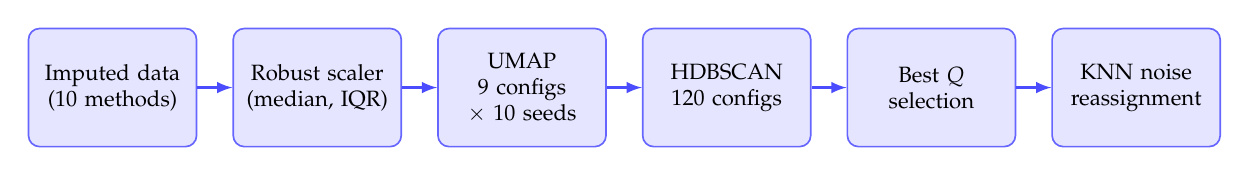
\begin{tikzpicture}[
  box/.style={draw=blue!60, line width=0.6pt, rounded corners,
              fill=blue!10, text width=1.9cm, minimum height=1.5cm,
              align=center, font=\footnotesize},
  arr/.style={->, line width=0.9pt, draw=blue!70, >=latex}
]
  \node[box] (imp) at (0,0)    {Imputed data\\(10 methods)};
  \node[box] (std) at (2.6,0)  {Robust scaler\\(median, IQR)};
  \node[box] (umap) at (5.2,0) {UMAP\\9 configs\\$\times$ 10 seeds};
  \node[box] (hdb) at (7.8,0)  {HDBSCAN\\120 configs};
  \node[box] (sel) at (10.4,0) {Best $Q$\\selection};
  \node[box] (knn) at (13.0,0) {KNN noise\\reassignment};
  \draw[arr] (imp) -- (std);
  \draw[arr] (std) -- (umap);
  \draw[arr] (umap) -- (hdb);
  \draw[arr] (hdb) -- (sel);
  \draw[arr] (sel) -- (knn);
\end{tikzpicture}%
}
\captionof{figure}[Pipeline overview]{This is an end-to-end clustering pipeline. Once the data have been imputed, they first pass through a robust scaler. Next, after being scaled, the imputed data pass into a UMAP hyperparameter grid with 10 random seeds for each of nine configurations, and the resulting embeddings that yield the highest silhouette value are retained. HDBSCAN then does the clustering in a 120-configuration sweep, based upon the composite quality measure $Q = \text{silhouette} \times (1 - \text{noise fraction})$, where all boundary noise points are assigned back to their respective cluster(s) via k-nearest neighbour. This entire process is run over each of the 10 possible imputation outcomes.}
\label{fig:pipeline_diagram}
\end{center}

\subsection{UMAP Parameter Grid}
I utilized Euclidean distance as the distance metric and \texttt{min\_dist}$=0.0$ to encourage separation between dense areas in the embedding.

\begin{table}[ht]
\caption{UMAP hyperparameter grid. All combinations of these values were put through their paces, for a total of 9 configurations.}
\label{tab:umap_grid}
\centering
\begin{tabular}{l l}
\toprule
\textbf{Parameter} & \textbf{Values} \\
\midrule
\texttt{n\_neighbors}  & 15, 30, 50 \\
\texttt{min\_dist}     & 0.0 \\
\texttt{n\_components} & 3, 5, 8 \\
\bottomrule
\end{tabular}
\end{table}

\subsection{HDBSCAN Parameter Grid}
Each UMAP embedding produced 120 possible candidate solutions (due to 120 different possible HDBSCAN configurations). To determine which configuration was "best," I employed a composite quality score that punished solutions with high silhouettes by allocating many assignments to noise:

\begin{equation}
Q = \text{silhouette} \times (1 - \text{noise proportion})
\label{eq:quality}
\end{equation}

\begin{table}[ht]
\caption{HDBSCAN hyperparameter grid. All listed value combinations were evaluated, giving me 120 configurations for each UMAP embedding.}
\label{tab:hdbscan_grid}
\centering
\begin{tabular}{l l}
\toprule
\textbf{Parameter} & \textbf{Values} \\
\midrule
\texttt{min\_cluster\_size}          & 500, 1000, 1500, 2000, 3000 \\
\texttt{min\_samples}                & 5, 10, 25, 50 \\
\texttt{cluster\_selection\_method}  & eom, leaf \\
\texttt{cluster\_selection\_epsilon} & 0.0, 0.1, 0.5 \\
\bottomrule
\end{tabular}
\end{table}

\subsection{Sweep Procedure}
The following procedures were employed for each imputed dataset. First, I preprocessed each dataset using a robust scaler. Second, I repeated each UMAP hyperparameter combination with ten random seeds, yielding ten embeddings per combination, and retained the embedding with the highest silhouette score. These repetitions assess sensitivity to stochastic initialisation; they are not folds of cross-validation. Third, I evaluated a grid of 120 HDBSCAN parameter configurations and selected the configuration yielding the highest quality score \(Q\). This is a hyperparameter sweep rather than 120-fold cross-validation. Fourth, I re-labelled observations previously labelled as noise. Noise points assigned by HDBSCAN were relocated to the nearest substantive cluster using k-nearest-neighbour similarity (\(k = 10\)) in UMAP space. This process yielded 100\% coverage. Re-labelling was allowed only when the silhouette decreased by less than 10\%, preserving separation between clusters.

\subsection{Worked Example}
Assume a hypothetical patient completes only those neuropsychological assessments related to orientation and digit span but fails to complete those related to Trail Making Test due to physical limitations or the delayed recall portion of the Rey Auditory Verbal Learning Test due to exhaustion. Upon application of Tier 1 filtering, however, the patient remains in the dataset with eligible variables only. The two missing scores are subsequently filled in by MICE based on observed information. The 14 variable-level scores are then subjected to winsorizing, aligned for direction, standardized, and weighted as defined in Section~\ref{sec:domain_scores} to produce six domain-composite scores. The robust scaler is applied to minimize the effect that floor and ceiling effects may have on aggregate measures. The resulting six-dimensional vector is then mapped into the cohort's UMAP representation space. The patient is then classified into one of three cognitive-severity tiers: Above Average, Near Normal, or Globally Impaired. If a patient falls into a sparse area of low density and was classified as noise, KNN reassignment utilizes neighboring assessments in UMAP-space (\(k = 10\)) and assigns them to the most closely located substantively-clustered tier. The final output includes a tier label and confidence score based on how often each imputation method agrees under hypothesis H2.

\section{Hypothesis Definitions}\label{sec:hypotheses}
\noindent \textbf{H1 (Stability and Discreteness of Cognitive Clusters)}. The UMAP + HDBSCAN pipeline is expected to identify at least two stable cognitive clusters for most imputation techniques. The stability criterion is met when the best solution from at least 8 of the 10 methods has an average silhouette $\geq 0.40$ and a pre-reassignment noise proportion $< 0.30$. These numerical thresholds evaluate partition quality and stability in the selected embedding; they do not by themselves establish that the clusters are discrete phenotypes. Discreteness is evaluated separately using profile shape, principal-component structure, separation in the original six-domain space, and sensitivity of the recovered cluster count.



\noindent \textbf{H2 (Robustness Across Imputation Techniques)}. Solutions for the clustering problems should show reasonable to high agreement among the imputation methods when the embedding geometry and partition model are held fixed. The primary discovery pipeline remains UMAP+HDBSCAN. For H2 only, I use a deliberately fixed secondary agreement diagnostic: a \(k\)-means labelling rule is trained on the MICE embedding and then applied unchanged to all other imputations. H2 is confirmed if the median pairwise ARI and NMI for each of the $\binom{10}{2} = 45$ combinations of methods exceeds 0.50. Although there is considerable flexibility in setting this threshold, it is greater than chance and implies substantial overlap in group membership under a common projection and labelling rule. This hypothesis therefore tests robustness of point assignments under a fixed reference structure; it does not require, or claim, that independently refitted UMAP+HDBSCAN solutions recover the identical number of tiers.



\noindent \textbf{H3 (Relationship Between Clinical Unit \& Cluster Membership)}. Cluster membership is expected to be related to clinical unit. For each imputation technique, a contingency table is created and a chi-square test of independence is conducted. H3 is confirmed if the relationship remains statistically significant at \(\alpha = 0.05\) after a Bonferroni adjustment and Cramér's \(V > 0.10\). As a sensitivity check for potential confounds, a Cochran-Mantel-Haenszel (CMH) test is performed, conditioned on an appropriate covariate.



\noindent \textbf{H4 (Clustering at Domain-Level vs. At Variable Level)}. I expect the cognitive features at the domain level to result in a clustering representation that is more interpretable and at least as well separated as the representation based on cognitive features at the variable level. H4 will be confirmed if the domain-level approach performs at least as well as or better than the variable-level approach on at least two of three metrics: (1) higher silhouette scores; (2) lower mean VIFs; and (3) lower condition numbers. Smaller values of VIF and condition number imply less multicollinearity and better numerical conditioning. Because cross-method agreement has already been assessed in H2, comparisons of feature representations are made in H4 exclusively.

\section{Statistical Tests and Validation}\label{sec:stats}

\subsection{Statistical Conventions}
Each statistical evaluation of hypotheses follows typical statistical practice. Each evaluation assesses the data relative to a null hypothesis \(H_0\), representing a "no-effect" baseline. The p-value is the probability of obtaining a test statistic as extreme as that obtained assuming \(H_0\) to be true; smaller p-values represent stronger evidence against \(H_0\). A predetermined significance level of \(\alpha = 0.05\) serves as the threshold for rejecting \(H_0\). For any parameter, a 95\% CI represents the range that would include the population parameter in 95\% of repeated random samples from the same population using the same methodology.



For applications of bootstrapping, observed data are randomly sampled with replacement to generate a simulated approximation of the sampling distribution of a statistic. The 2.5th and 97.5th percentiles of that simulated distribution define the bootstrap CI. A z-score quantifies how many standard deviations away from the mean of a specified reference distribution a given value lies. With respect to the psychological testing instruments employed here, standardized testing permits scores derived from different instruments to be compared.



Cohen defined standards for interpreting the magnitude of effects, specifically for standardized differences, i.e., Cohen's \(d\). Specifically, \(d = 0.20\) is interpreted as a small effect size, \(d = 0.50\) as a medium-sized effect, and \(d = 0.80\) as a large effect size. When applying Cramér's V as an effect size for evaluating chi-squared tests, \(V = 0.10\) is interpreted as a small effect size, \(V = 0.30\) as a medium effect size, and \(V = 0.50\) as a large effect size.

\begin{equation}\label{eq:cohend}
d=\frac{\bar{x}_1-\bar{x}_2}{s_p},\qquad s_p=\sqrt{\frac{(n_1-1)s_1^2+(n_2-1)s_2^2}{n_1+n_2-2}},
\end{equation}

\subsection{Tests and Validation Procedures}
\noindent \textbf{Bootstrap Stability}. I conduct an assessment-level bootstrap stability analysis for every imputation method using \(B = 50\) resamplings. Assessments are sampled as rows, so repeated observations from the same patient are not grouped during resampling. For each resampling, I refit HDBSCAN on the cached UMAP embeddings, recording the median silhouette (Eq.~\ref{eq:silhouette}) and pre-KNN noise proportions. Pre-KNN noise proportion is equal to the proportion of observations that do not belong to any meaningful cluster:

\begin{equation}\label{eq:noise}
\text{noise}=\frac{1}{n}\bigl|\{\,i:\text{label}(i)=\text{noise}\,\}\bigr|,
\end{equation}

This is also the value used in defining quality function \(Q\) (Eq.~\ref{eq:quality}). According to H1's pre-defined conditions, a method will be deemed successful if its median silhouette is larger than or equal to 0.40 and its pre-KNN noise proportion is less than or equal to 0.30; at least 8 of the 10 methods will need to satisfy both conditions. To evaluate per-cluster stability, I apply Hennig (2007)'s matching algorithm to the pre-KNN labels using the default threshold (i.e., 0.7).



\noindent \textbf{Pairwise Agreement}. In order to remove variability caused by refitting other parts of the pipeline, I employ a shared reference-pipeline strategy. This is a secondary sensitivity analysis, not the clustering procedure used to discover the primary tiers. One StandardScaler, one UMAP model, and one \(k\)-means model with \(k=3\) are trained on MICE-imputed domain scores. The remaining methods are then standardized, projected onto this MICE-trained pipeline, and classified using that same MICE-trained \(k\)-means model. The use of \(k\)-means here is intentional: it supplies a fixed labelling function so that the imputed values are the only element varying across methods. This design tests whether assessments produced by different imputation methods land in similar regions under a fixed embedding and partition; it does not test whether a newly fitted UMAP+HDBSCAN pipeline would reconstruct the same geometry, density hierarchy, or number of tiers from each imputed dataset. It creates the ARI (Eq.~\ref{eq:ari}) and NMI (Eq.~\ref{eq:nmi}) matrices comparing each method to each other shown as heatmaps in Chapter~\ref{Chapter4}. Confidence for each assessment is defined as:

\begin{equation}\label{eq:consensus}
\mathrm{conf}(i)=\max_{\ell}\frac{1}{M}\sum_{m=1}^{M}\mathbf{1}\!\left[\text{label}_m(i)=\ell\right],
\end{equation}

High-confidence assessments are those whose assessments were placed into the mode cluster by at least \(M/10 = 0.8 \times 10 = 8\) methods.



\noindent \textbf{Chi-Square Test, Cramér's V, CMH Test}. Contingency tables arise from cross-classifying two categorical variables - e.g., cluster assignment and clinical unit - giving joint counts. Pearson's Chi-Square Test evaluates observed counts \(O_{ij}\) against expected counts \(E_{ij}\) under the null hypothesis that the two variables are independent:

\begin{equation}\label{eq:chi2}
\chi^2=\sum_{i=1}^{r}\sum_{j=1}^{c}\frac{(O_{ij}-E_{ij})^2}{E_{ij}},\qquad E_{ij}=\frac{O_{i\cdot}\,O_{\cdot j}}{n},
\end{equation}

with \(O_{i\cdot}\) and \(O_{\cdot j}\) denoting row sums and column sums, respectively. The test statistic is referenced against a Chi-Square distribution with \((r - 1)(c - 1)\) degrees of freedom to yield the p-value. Cramér's V is used to render association statistics scale-free for sample-size purposes, since it takes on values between zero and one:

\begin{equation}\label{eq:cramersv}
V=\sqrt{\frac{\chi^2}{n\,(k-1)}},\qquad k=\min(r,c),
\end{equation}

The Cochran-Mantel-Haenszel Test extends Pearson's Chi-Square Test for data organized into strata (e.g., diagnosis subgroups). The CMH Test determines whether the association between cluster assignments and clinical units remains significant even when stratifying by an appropriate covariate:

\begin{equation}\label{eq:cmh}
\chi^2_{\mathrm{CMH}}=\frac{\bigl(\sum_{h}(a_h-\mathbb{E}[a_h])\bigr)^2}{\sum_{h}\operatorname{Var}(a_h)}.
\end{equation}

\noindent \textbf{Patient-Grouped Multinomial Sensitivity Analysis}. Because association statistics do not establish predictive performance, I also compared two regularised multinomial logistic models for detailed clinical-unit assignment. The baseline model used the broad diagnostic grouping supplied by the clinical-unit lookup; the augmented model added cognitive-severity tier. Units represented by fewer than 50 unique patients were combined into an ``other units'' category, leaving 17 outcome classes. Five-fold stratified group cross-validation kept every assessment from the same patient in a single fold. Held-out multinomial log loss was the primary performance measure, with accuracy and macro-F1 reported descriptively. The difference in out-of-fold log loss was bootstrapped 1{,}000 times by patient. Because the broad diagnostic grouping is derived from the same lookup as detailed clinical unit, this model is a sensitivity analysis of incremental classification performance rather than independent external validation.



\noindent \textbf{Variance Inflation Factor}. To quantify multicollinearity in regression models, VIF is used. For any variable \(j\), it is defined as:

\begin{equation}\label{eq:vif}
\mathrm{VIF}_j=\frac{1}{1-R_j^2},
\end{equation}

where \(R_j^2\) denotes the coefficient of determination when regressing \(j\) on all other predictors. Any value exceeding 10 constitutes grounds for concern, and influences interpretation both at the variable level and in subsequent analyses at the domain level.

\subsection{Implementation}

\begin{sloppypar}
The historical analyses were implemented in Python (version 3.13); the patient-level extension uses a separate pinned Python 3.12 environment.
Imputation used
\texttt{scikit-learn} (KNN, NMF),
\texttt{fancyimpute} (SoftImpute, EM),
\texttt{miceforest} (MICE, PMM), and
\texttt{missforest} (MissForest).
DAE and VAE used \texttt{PyTorch}.
UMAP used \texttt{umap-learn};
HDBSCAN used the \texttt{hdbscan} library.
Statistical tests used \texttt{scipy.stats} and \texttt{statsmodels}.
Validation metrics used \texttt{scikit-learn}.
The analysis code and dashboard are available at
\url{https://github.com/zkunos/thesis_project}.
\end{sloppypar}

%----------------------------------------------------------------------------------------

\section{Patient-Level Clustering Extension}\label{sec:extension_methods}

An exploratory follow-up to this study was conducted on October 15, 2026. The analysis explored whether the existing historical severity categories represent stable subcategories with regard to different ways the data can be represented, with regard to how the data may have been missed, and when using different sampling units. The findings from this study are supplemental to those found in H1-H4, but do not redefine those hypotheses. The supporting literature was limited to journal articles published between October 15, 2025 and October 15, 2026. Articles used in comparisons of mixture modeling of missing data, multi imputation ensemble approaches and techniques for diagnosing clusterability (in addition to comparative longitudinal analysis) included \textcite{tong2025mixturemissing,tomo2026ensemble,neville2026clusterability,julia2026longitudinal} and provided further rationale for determining if there existed structure in the measure feature space based upon distortions present in UMAP embeddings \parencite{chen2026umapartifacts}. None of these articles validated a particular type of ABI or established which methodology would produce better results than the historical methodology.

\subsection{Cohort and Discovery--Validation Split}

We identified an eligible population of 17,406 evaluations performed on 7,285 individuals, across the 14 retained cognitive tests. Identifiers for patients link repeated evaluations; there are no duplicated patient-evaluation-time combinations. No validated identifiers exist for defining episodes of injury. One patient reported differing ages at injury across assessments and was removed from trajectory modeling based on their evaluation history.

Patient assessments were ordered by time post-injury, and each patient's first eligible evaluation was used in the cross-sectional aspect of this study. When determining the order of assessments for multiple evaluations within a single patient, source row ordering is used to break ties deterministically. In a fixed random split using seed \#20261015, 5,828 patients were randomly assigned to the training set (discovery) and 1,457 patients were randomly assigned to the testing set (validation). Since each patient provides only one index profile, no patient appears in both groups. This allows us to estimate structure in patient index profiles while we describe assessment state across follow-up in the historical analysis. It has also already been noted that the 14 feature variables chosen for use in this research were those same as the feature variables used in our previous historical analyses for the entire cohort of patients. Thus, the division as described does not represent an independent validation of how we chose these feature variables.

Eligibility required at least one observed retained test. A separate sensitivity analysis evaluated the impact of sparse measurements of patient assessment profiles. Specifically, it used index evaluations where at least seven of the 14 retained tests had been measured.

\subsection{Shared Preprocessing and Feature Representations}

Data in discovery datasets establish the 1st and 99th percentiles, means and standard deviations for each test. Values are clipped at those percentile bounds, and timed \texttt{ATMTA} scores are sign-inverted. Standardization is employed to create larger values associated with higher achievement. This transformation leaves missing entries unchanged. For completed-data branches, a bounded Bayesian chained-equations imputer was fitted on discovery patients and used to impute missing values for validation patients. An iterative, deterministic reference model was created using 15 iterations. An additional sensitivity study utilizing 50 iterations was conducted to assess convergence of the iterative algorithm. Note that this imputation method differs from the historical \texttt{miceforest} implementation and has its own modeling assumptions.

The completed standardized tests were grouped by six domains based on the frequency of each test's administration. Each domain's weight is determined by the frequency of each test being administered to the discovery dataset; however, the weights have been normalized within each domain. Domain median and inter-quartile range (robust scaling) derived from the discovery dataset were utilized to calculate the reference distance representation. The comparator options include either the 14 completed tests or the 5 non-orientation domains. Following removal of the first principal component derived from the discovery patient data, a five-dimensional PCA basis was developed. Residual representation represents a diagnostic tool for identifying potential shape differences amongst profile groups. Therefore, residual representation may remove valid signals as well as common variability.

After examining discovery-set variances, an additional scaling sensitivity was introduced in which each domain has a variance of one. This sensitivity is designed to evaluate the influence of domains having "ceiling" issues which tend to have very narrow ranges around their midpoints. By evaluating identical label sets in both geometric models, we can separate differences in how the data are divided from differences in how silhouette is calculated. The transformations applied to the validation patients remain unchanged from those originally estimated in the discovery data.

In terms of analyzing each patient individually, the patient level analysis utilizes clipping, direction alignment and test standardization before the values are then combined. Previous supplementary analyses utilized multiple imputation and complete case comparison methodologies to aggregate raw tests. Consequently, the prior results that were provided as part of this study used a different preprocessing methodology than the patient-level extension. Controlled comparisons using identical completed test values assess the impact of aggregation without recalculating all the previous H1-H4 statistics.

\subsection{Original-Space and Incomplete-Data Models}

The clustering techniques k-means and PAM (sampled partitioning around medoids) were evaluated for values of $k=2,\ldots,8$. PAM utilizes CLARA-style sampling on three sets of 400 discovery patient data, followed by a BUILD/SWAP optimization within each sample. Additionally, the Gaussian Mixture Model was evaluated for $k=1,\ldots,8$. Both full and tied covariance matrices were used. HDBSCAN was run against the data for two sets of parameters: (a) minimum cluster size of either 100 or 300; and (b) \texttt{min\_samples}=20. For the comparison utilizing UMAP, three-dimensional representations were employed, along with 15 or 50 nearest neighbor values with a \texttt{min\_dist}=0 before applying the same HDBSCAN parameters as above. In terms of assigning validation patients to clusters, this was performed using the fitted centers, medoids, mixture probabilities, or UMAP transformation and HDBSCAN approximate prediction.

Models to fit each representation/method were selected based upon the highest discovery silhouette for partition/density methods and lowest discovery BIC for Gaussian mixtures. When applicable, fits had to converge and every group had to contain at least two percent of the discovery patients. Silhouettes were computed in the respective original representation (including UMAP-derived labels). Up to 2,000 randomly sampled observation discovery scores were used when computing discovery scores. All available assignments were used when calculating validation scores. Noise was excluded from silhouette, and coverage was reported separately. Scores from different feature geometries are not a common performance scale. A silhouette search for $k\geq2$ does not determine whether there exists a group relative to an existing one population model.

The incomplete-data mixture models were fitted to 14 transformed test results using expectation maximization (EM). Missing coordinates were integrated out in the observed-data likelihood. There were three restricted families used: (a) Gaussian; (b) $t$-distributions with df = 4 \& 10; (c) contaminated normal with a 90\% normal core and tenfold covariance inflation for the remaining 10\%. Each of the above mentioned families were estimated with $k=1,\ldots,8$, using two different starting conditions, with a 120-iteration limit or convergence when the change in log likelihood per observation was below $10^{-5}$, and an eigenvalue floor of 0.02 to the dispersion matrix. Due to scale matrices being used within the $t$ family estimation process, the eigenvalue floor also served as a scale-matrix floor. Mean Imputation was the only method used for developing starting values. Verification of these implementations has been done through computational verification. These are simplified versions of the full \textit{MixtureMissing} package \parencite{tong2025mixturemissing} and lack some functionality.

BIC, entropy-penalized ICL, convergence, validation observed-data log likelihood and posterior membership probabilities were recorded for each fit. Selected fits had to converge and assign at least 2\% discovery membership to each component. Likelihood measures are compared only among fits sharing the same transformation into the 14-dimensional space. Because continuous distributions are being used to approximate discrete/bounded scores, any additional groups could represent ceiling effects, skewness, or tailing rather than separate subpopulations of patients.

\subsection{Independent Refitting, Consensus and Cluster Tendency}

Twenty stochastic imputed datasets were generated from bounded Bayesian posterior draws, using ten chained-equations iterations per dataset. K-means and sampled PAM were fitted separately with fixed $k=2,3,4$, refitting domain scaling for each draw. Ensemble PAM used two samples of 300 discovery patients. Each assignment vector contained the same 1,457 validation patients. Agreement across draws was measured by mean pairwise ARI and empirical 5th-95th percentiles. These are not confidence intervals because partition pairs share fits. A separate discovery-silhouette k-means screen assessed $k=2,\ldots,8$ in each run.

Fifty runs used 80\% subsamples of discovery patients to fit preprocessing, imputation, scaling, and the fixed k=3 group k-means. Fifty additional runs were made where the clustering seed varied while the input vector was kept constant. The patient sampling variability was assessed by computing the held-out ARI and matched per-cluster Jaccard indices to differentiate it from initial condition variability. Additional sensitivity checks assessed the effects of mean versus KNN imputation, no clipping, stricter availability requirements for tests, and independent fitting of the validation partitions.

Finally, I compared average-linkage co-assignment, greedy mean-NMI, and generic NMF as three approaches to summarize the descriptive properties of held-out assignment vectors using methods similar to \textcite{tomo2026ensemble}. Although these are the native implementations of those methods, they are not an exact replication of that paper. Additionally, consensus regarding the validation assignments does not constitute a predictive model which has been separately validated. Collapsed groups and nonconvergence are reported.

The results from the PCA/DIP diagnostic analysis were then compared to a matched-size screening set of 1,000 discovery patients and 100 separate reference samples that were each constructed by sampling from a single Gaussian copula. The empirical discrete marginal distributions as well as the missingness joint mask created through the application of resampling techniques were preserved for each. Additionally, each of these 100 reference datasets were subjected to the exact same processing procedures used on the initial dataset. Specifically, this included: preprocessing; estimation of missing data; and K-Means Clustering Analysis with varying cluster counts ($k=2,\ldots,8$). The tail fraction comparisons include both the observed Max Silhouette and PC1 Dip Statistics when compared to those present within the reference distribution(s). The method of comparison described above is known as ``descriptive fitted-reference calibration''. The simulation missingness masks are generated independently of the simulated data and selection across all model families is not repeated. In addition, there is a two group positive control check to check basic recovery. However, neither of the screens or the projection based modality test identify clinical subtypes \parencite{neville2026clusterability}.

\subsection{Patient Trajectories and Reproducibility}

To qualify for the longitudinal sample, a patient had to meet all of the following requirements. There had to be at least three visits with seven or more observed tests and at least three distinct time points. The interval between the first and last eligible observation could be no shorter than 0.25 years and no longer than five years. Recorded age at injury also had to be consistent across assessments.

I developed a longitudinal cognitive score using the frozen index-discovery preprocessing, imputer and robust-space PC1. The score was oriented towards better performance and divided by its index-discovery standard deviation. Time was measured in years since the first eligible time point. Each patient kept their original discovery or validation status throughout the longitudinal analysis.

I modelled the data using Gaussian linear trajectory mixture models. The patients' random intercepts and slopes were integrated into the models. Models varying in number of classes (from 1 to 4) were fit. Random-effects covariance and residual variance were shared across all of the classes. For each model, three different sets of initial values were tested and up to 300 EM iterations were allowed. Only models that converged as well as had an average posterior probability of at least 0.05 in each of their respective classes could be evaluated with respect to discovery BIC. Therefore, any model that failed to converge during its estimation procedure or had an average posterior probability < 0.05 in any particular class would be eliminated from consideration. To provide a point of comparison, we also ran a one-class model in which there was a continuous random effect. Additionally, patient subsampling was conditional on selecting more than one class. Rather than determining how much of the identified pattern(s) could be due to underlying causal mechanism(s), we wanted to determine what other observed patterns of interest existed. We did not run analyses of nonlinear trajectories. Also, we did not utilize the recently developed multivariate contaminated longitudinal model. Recent studies of longitudinal data motivate separating initial value from rate of change \parencite{julia2026longitudinal}.

All analyses were performed using Python 3.12.14 with fixed version numbers for all dependencies, reproducible random seed states and as previously stated, model grids. Eight numerical tests evaluated the reference likelihoods, recovery of missing data, monotonicity of EM log-likelihood, preprocessing directionality, selection of the medoids, integration over trajectory likelihoods and evaluation of the overall ensemble objective function. No independent rehabilitation outcome was available, so predictive clinical utility remains untested.


% Chapter 4 (Shortened)

\chapter{Results}\label{Chapter4}

The chapter first presents the assessment-level results, followed by the patient-level extension in Section~\ref{sec:extension_results}. The earlier supplementary multiple-imputation and complete-case comparisons used raw-test aggregation. Their quoted results therefore describe a different preprocessing specification from the direction-aligned, standardized domain construction used in the extension and are not directly comparable with it.

%----------------------------------------------------------------------------------------
%	SECTION 1
%----------------------------------------------------------------------------------------

\section{Exploratory Data Analysis}
Following Tier-1 filtering (Chapter~\ref{Chapter3}) and removal of all assessments lacking any cognitive measures, the remaining dataset consisted of 17{,}406 assessments from 7{,}285 patients. The resulting matrix included cognitive variables amounting to 14 variables over six domains. The percentages of missing values are provided in Table~\ref{tab:missing_descriptive}.



Data availability is inconsistent. The missingness levels vary from 0.7\% for Orientation items through to 27.8\% for ATMTA. Therefore, complete-case analysis would lose approximately half of the total clinical sample (46.9\%) and risk selection bias \parencite{rubin1976inference}. Consequently, data imputation was adopted to conserve the entire clinical sample.



From a co-occurrence heatmap (not shown), blocks of variables are identified that are missing simultaneously, showing structured missingness but not establishing a missing-at-random mechanism \parencite{rubin1976inference,little2019statistical}. Dependency among missing values thus supports the application of conditional imputation rather than naive substitution. Within-domain correlation coefficients are generally high, whereas cross-domain relationships appear less prominent, suggesting common variance due to general cognitive ability \parencite{lezak2012neuropsychological}. Subsequent clustering results illustrate this common variance dimension explicitly.

\begin{table}[ht]
\caption{Missingness summary for the 14 eligible neuropsychological variables after Tier~1 filtering. The final row reports the number of complete cases (rows with no missing values across all 14 variables).}
\label{tab:missing_descriptive}
\centering
\small
\begin{tabular}{l l r r r}
\toprule
\textbf{Variable} & \textbf{Domain} & \textbf{$N$ Observed} & \textbf{$N$ Missing} & \textbf{Missing \%} \\
\midrule
\texttt{OTEMPS}          & Orientation        & 17{,}286 &   120 &  0.7 \\
\texttt{OPERSONA}        & Orientation        & 17{,}284 &   122 &  0.7 \\
\texttt{OESPAI}          & Orientation        & 17{,}282 &   124 &  0.7 \\
\texttt{ASPAN}           & Attention          & 15{,}611 & 1{,}795 & 10.3 \\
\texttt{MRAVLT075}       & Memory             & 15{,}523 & 1{,}883 & 10.8 \\
\texttt{MDIGITS}         & Memory             & 15{,}373 & 2{,}033 & 11.7 \\
\texttt{FEPMR}           & Executive Function & 14{,}682 & 2{,}724 & 15.6 \\
\texttt{LCOMPRENSIOTB}   & Language           & 14{,}686 & 2{,}720 & 15.6 \\
\texttt{LDENOMINACIOTB}  & Language           & 14{,}677 & 2{,}729 & 15.7 \\
\texttt{LREPETICIOTB}    & Language           & 14{,}634 & 2{,}772 & 15.9 \\
\texttt{MRAVLT015}       & Memory             & 14{,}281 & 3{,}125 & 18.0 \\
\texttt{MRAVLT015R}      & Memory             & 14{,}199 & 3{,}207 & 18.4 \\
\texttt{VPIMATGES}       & Visuoperception    & 12{,}992 & 4{,}414 & 25.4 \\
\texttt{ATMTA}           & Attention          & 12{,}575 & 4{,}831 & 27.8 \\
\midrule
\multicolumn{3}{l}{\textbf{Complete cases (all 14 variables observed)}} & \multicolumn{2}{r}{\textbf{9{,}245 (53.1\%)}} \\
\bottomrule
\end{tabular}
\end{table}

In Figure~\ref{fig:missingness_barplot}, missingness levels for each cognitive variable are displayed in descending order. Highly specialized assessments consistently demonstrate higher levels of missingness than routine screening measures \parencite{lezak2012neuropsychological}.

\begin{center}
\centering
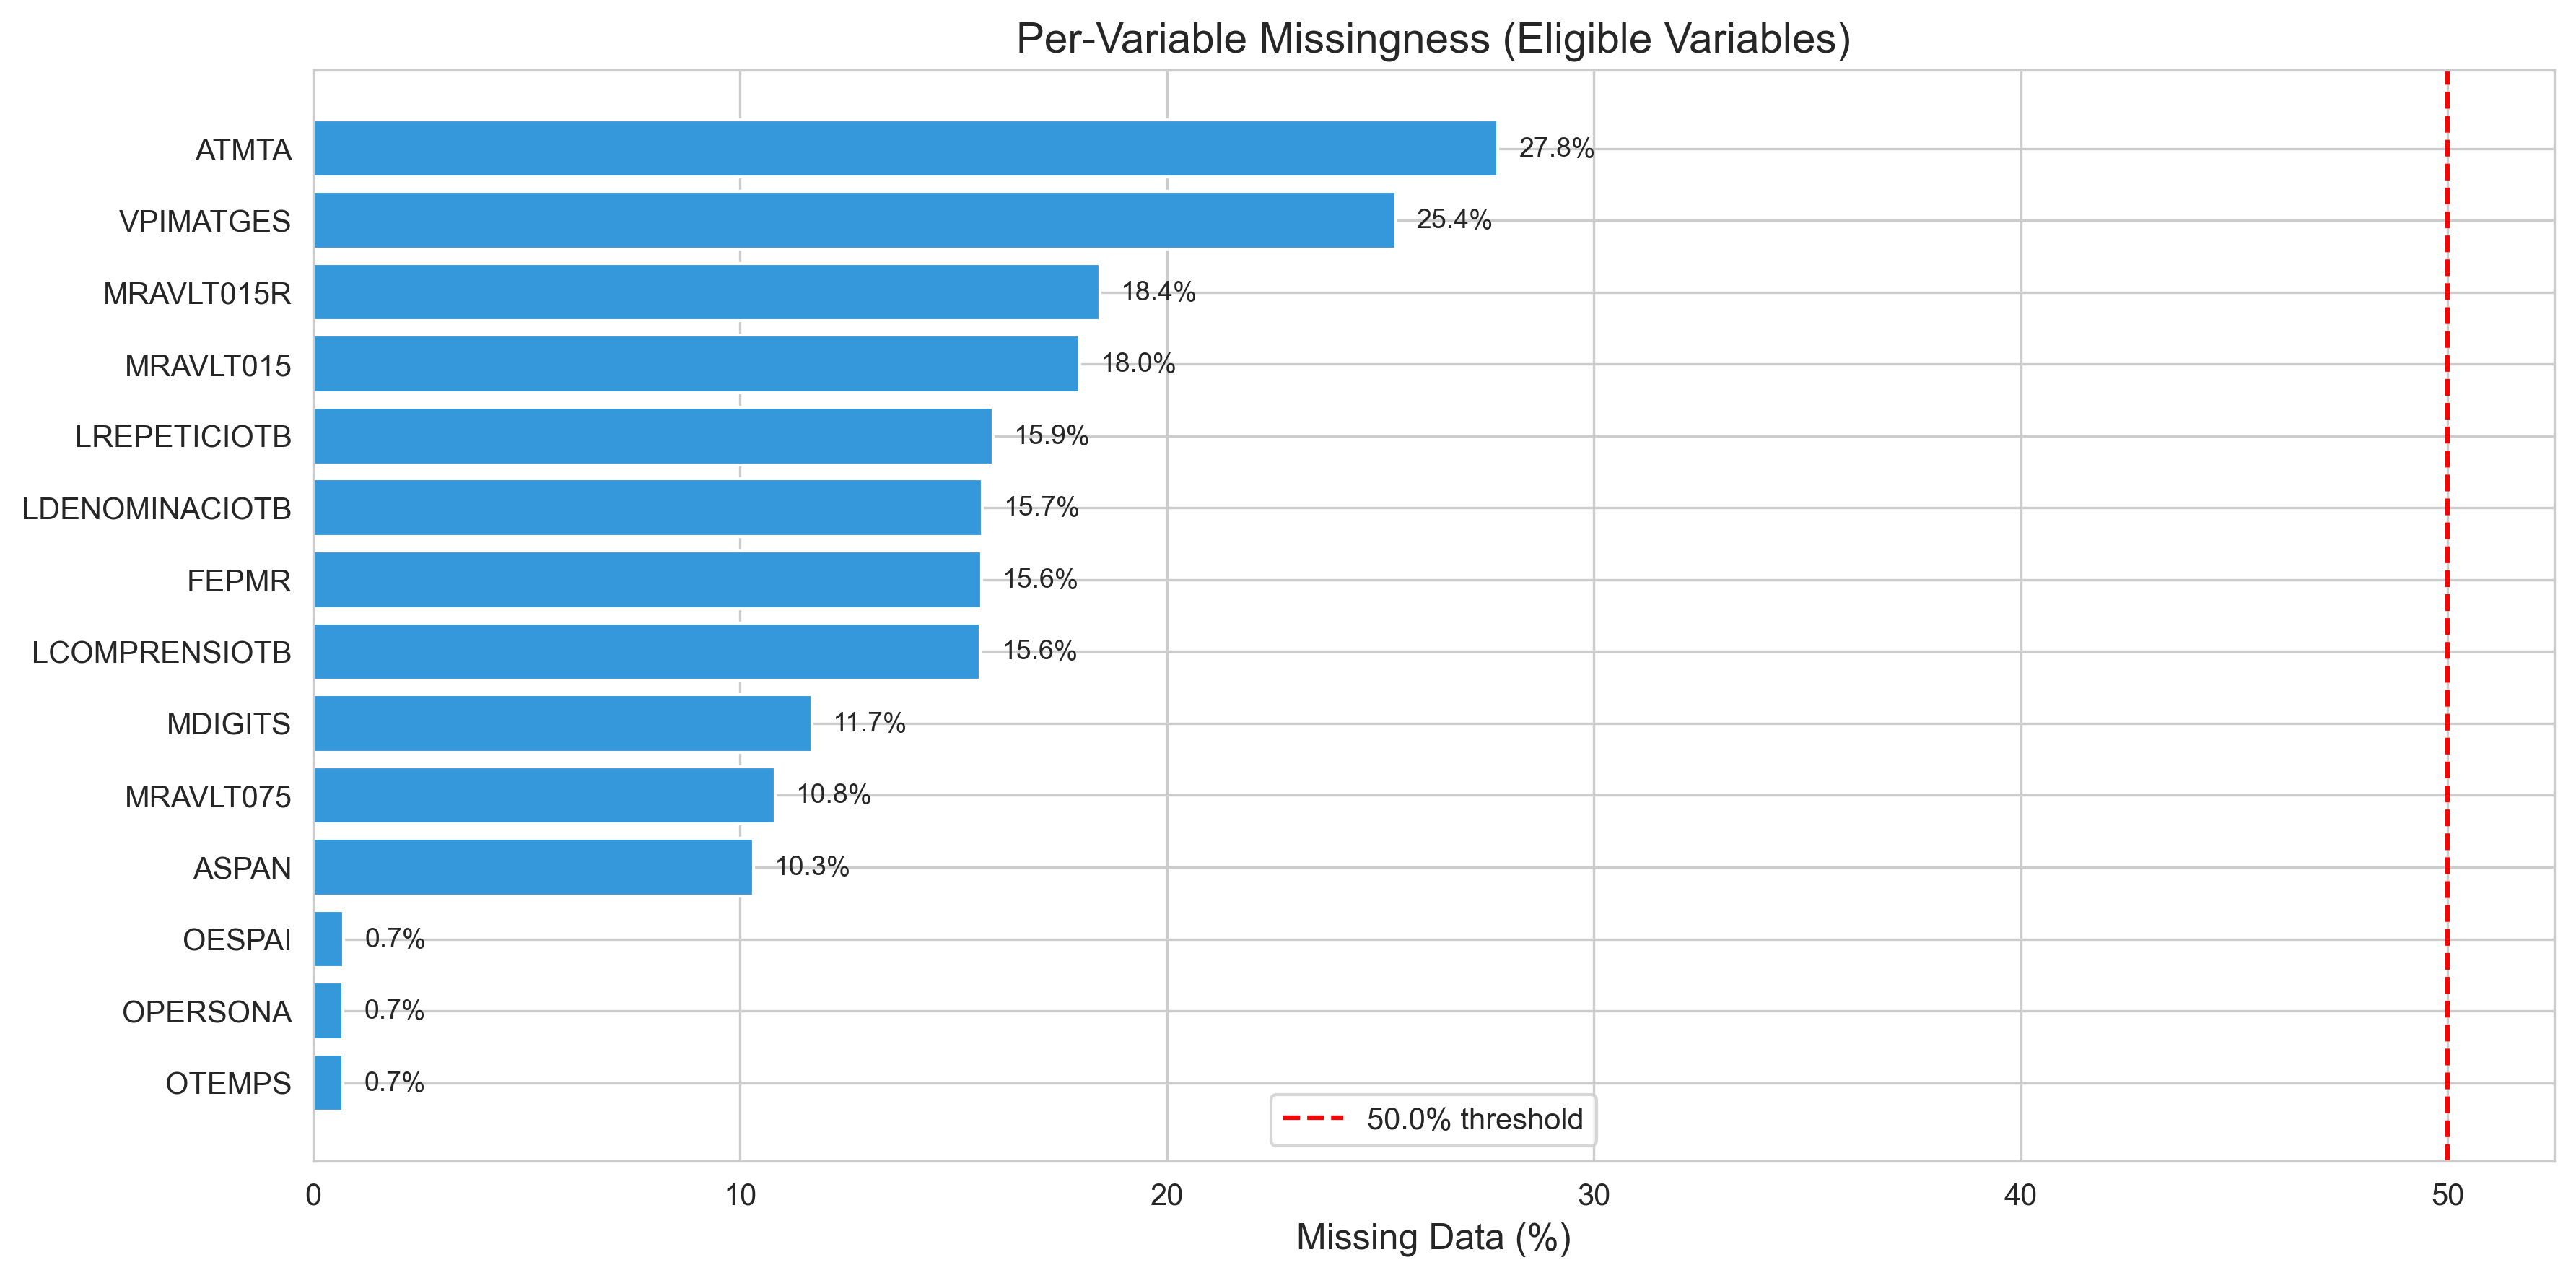
\includegraphics[width=0.9\textwidth]{Figures/missingness_barplot.png}
\captionof{figure}[Missingness rates by variable]{Missingness bar plot for all cognitive variables, ordered by missingness rates. Missingness rates were higher among the specialised assessments compared to the routine screening assessments.}
\label{fig:missingness_barplot}
\end{center}

\section{Imputation Results}
Prior to conducting clustering evaluations on their respective datasets, I tested all ten imputation techniques represented in Figure~\ref{fig:imputation_comparison} and Figure~\ref{fig:imputation_comparison_b}. Due to compression of variance \parencite{rubin1987multiple}, Mean Imputation behaves differently from all other methods. All nine remaining methods maintain closer adherence to marginal distributions. Discrete structure retention is greater among donor-based methods like KNN and PMM than among model-based approaches including MICE, MissForest and EM that produce smoothed continuous reconstructions.

\begin{center}
\centering
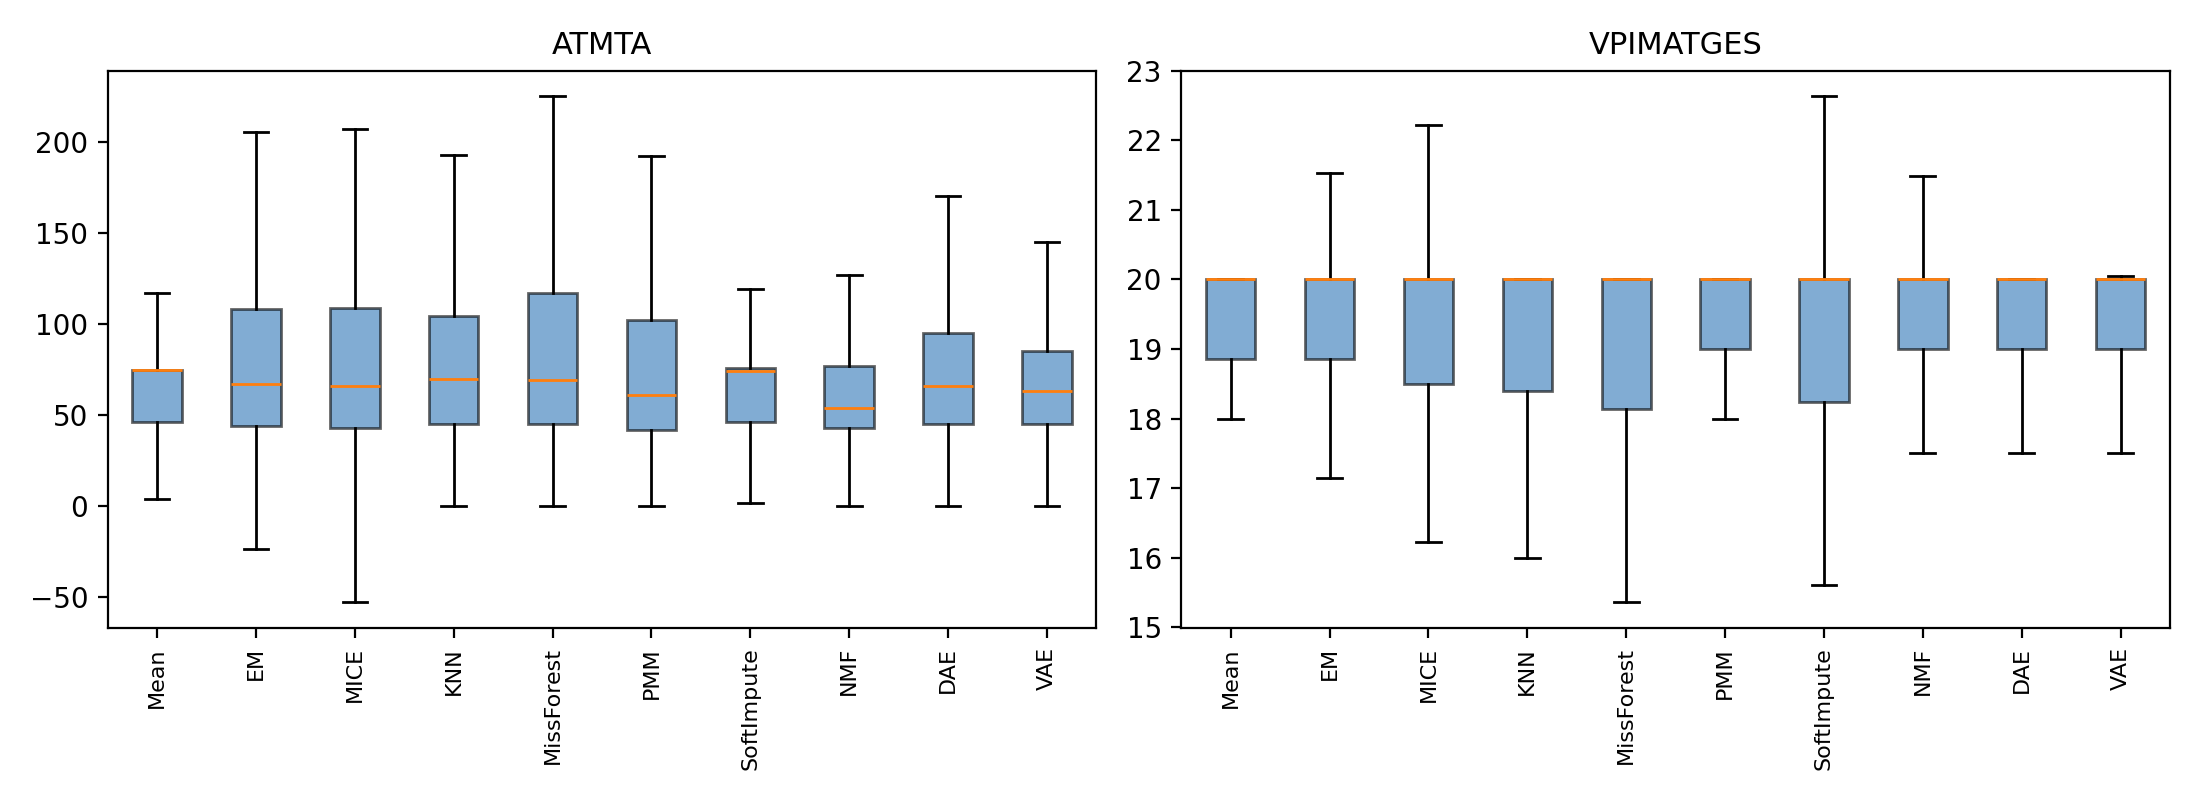
\includegraphics[width=0.95\textwidth]{Figures/imputation_comparison_boxplots_a.png}
\captionof{figure}[Imputation comparison (ATMTA, VPIMATGES)]{Comparison of distributions for each of the 10 different imputation methods for ATMTA and VPIMATGES. Mean imputation reduces variance whereas model-based methods maintain the distributional characteristics of the original data.}
\label{fig:imputation_comparison}
\end{center}

\begin{center}
\centering
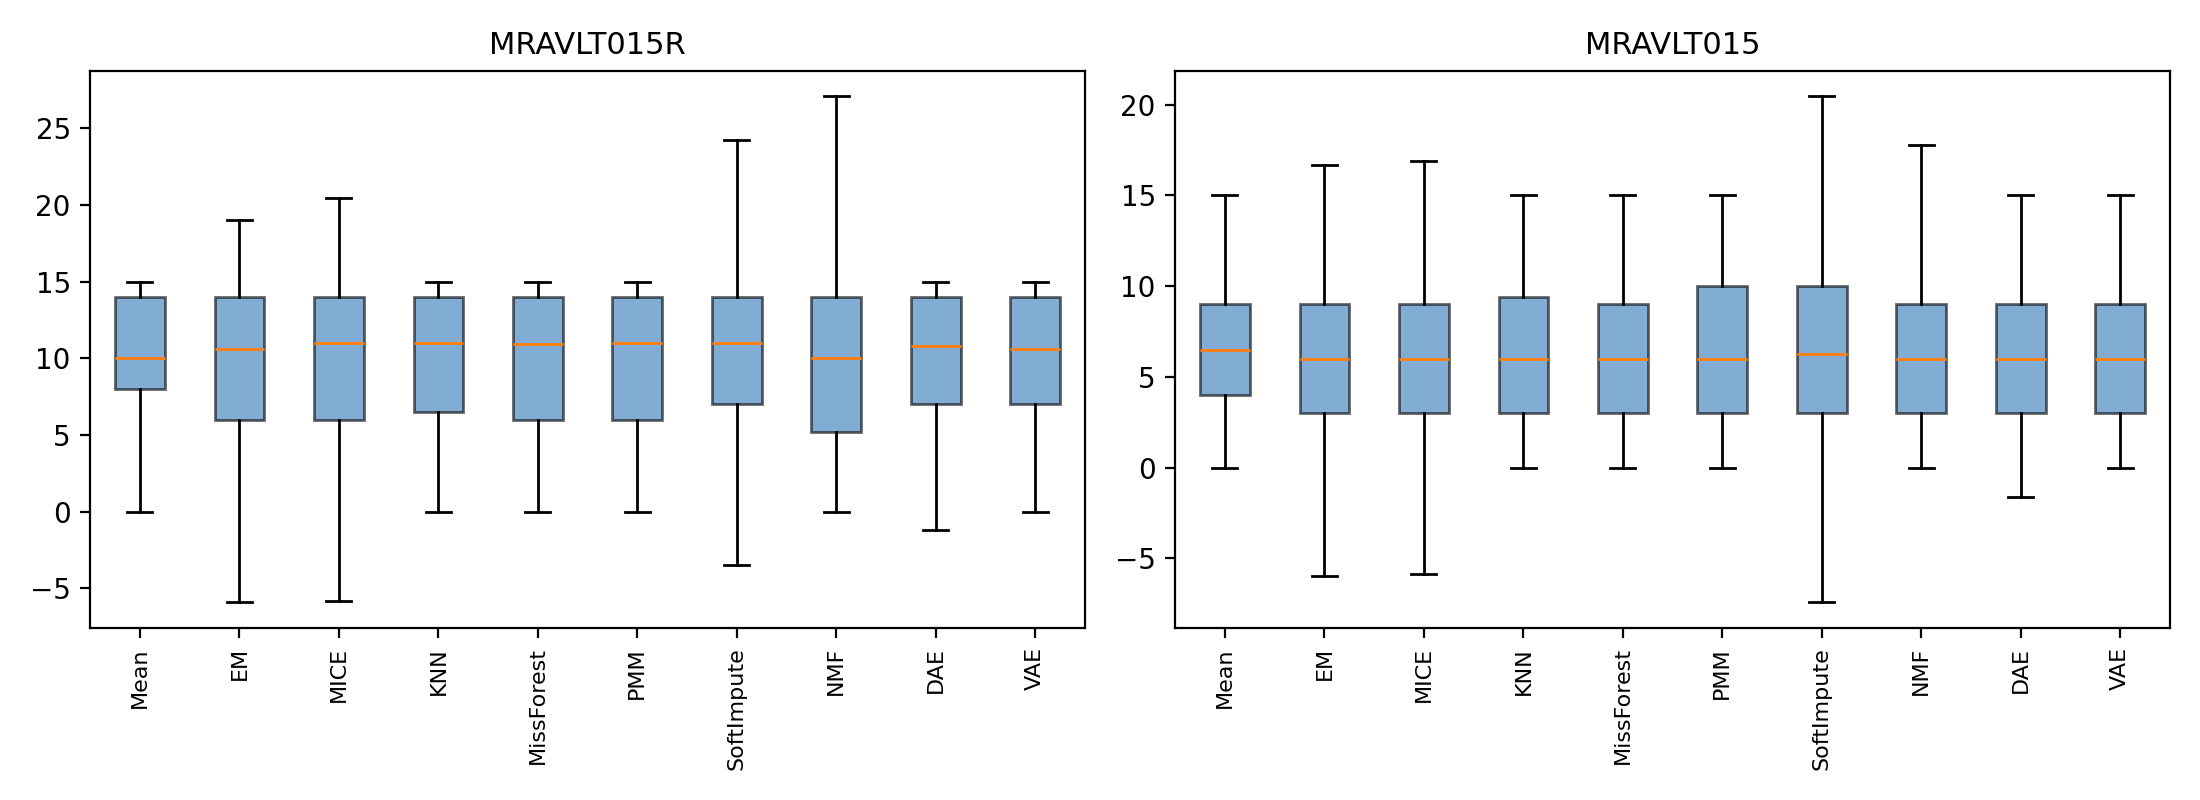
\includegraphics[width=0.95\textwidth]{Figures/imputation_comparison_boxplots_b.png}
\captionof{figure}[Imputation comparison (MRAVLT015R, MRAVLT015)]{Comparison of distributions for MRAVLT015R and MRAVLT015. Deep learning models (DAE, VAE) closely approximate model-based methods.}
\label{fig:imputation_comparison_b}
\end{center}

\section{Baseline and Primary Clustering}
I first fitted K-means and Gaussian mixture baselines across \(k=2\) through \(k=6\). Neither produced a clear discrete optimum: the K-means elbow lacked a pronounced break, and silhouette was highest at \(k=2\) but declined as additional groups were introduced. These baselines motivated examination of density structure; they were not treated as evidence that natural cognitive classes existed.

I selected HDBSCAN because it can recover irregularly shaped dense regions, represent low-density observations as noise, and examine cluster persistence across a hierarchy without requiring a fixed value of \(k\). This combination was appropriate for routine clinical data in which boundary cases may not fit cleanly into a group. UMAP was repeated across ten random seeds per parameter configuration, and HDBSCAN was evaluated over the 120-configuration grid described in Chapter~\ref{Chapter3}. The comparison of t-SNE and UMAP in Figure~\ref{fig:tsne_umap} is descriptive: it illustrates how the selected assignments appear under two projections, but it is not an independent test of cluster existence or discreteness.

\begin{sloppypar}
For the UMAP+HDBSCAN combination, the hyperparameters I settled on were: \texttt{n\_components}$=8$, \texttt{n\_neighbors}$=15$, and \texttt{min\_dist}$=0.0$ for UMAP (to allow for tight packing in the embedding space \parencite{mcinnes2018umap}); and for HDBSCAN, \texttt{min\_cluster\_size}$=1000$ and \texttt{min\_samples}$=50$ with \texttt{cluster\_selection\_method}$=\text{eom}$ and \texttt{epsilon}$=0.0$. I chose a large cluster size to ensure that only substantive groupings are retained.
\end{sloppypar}

\begin{center}
\centering
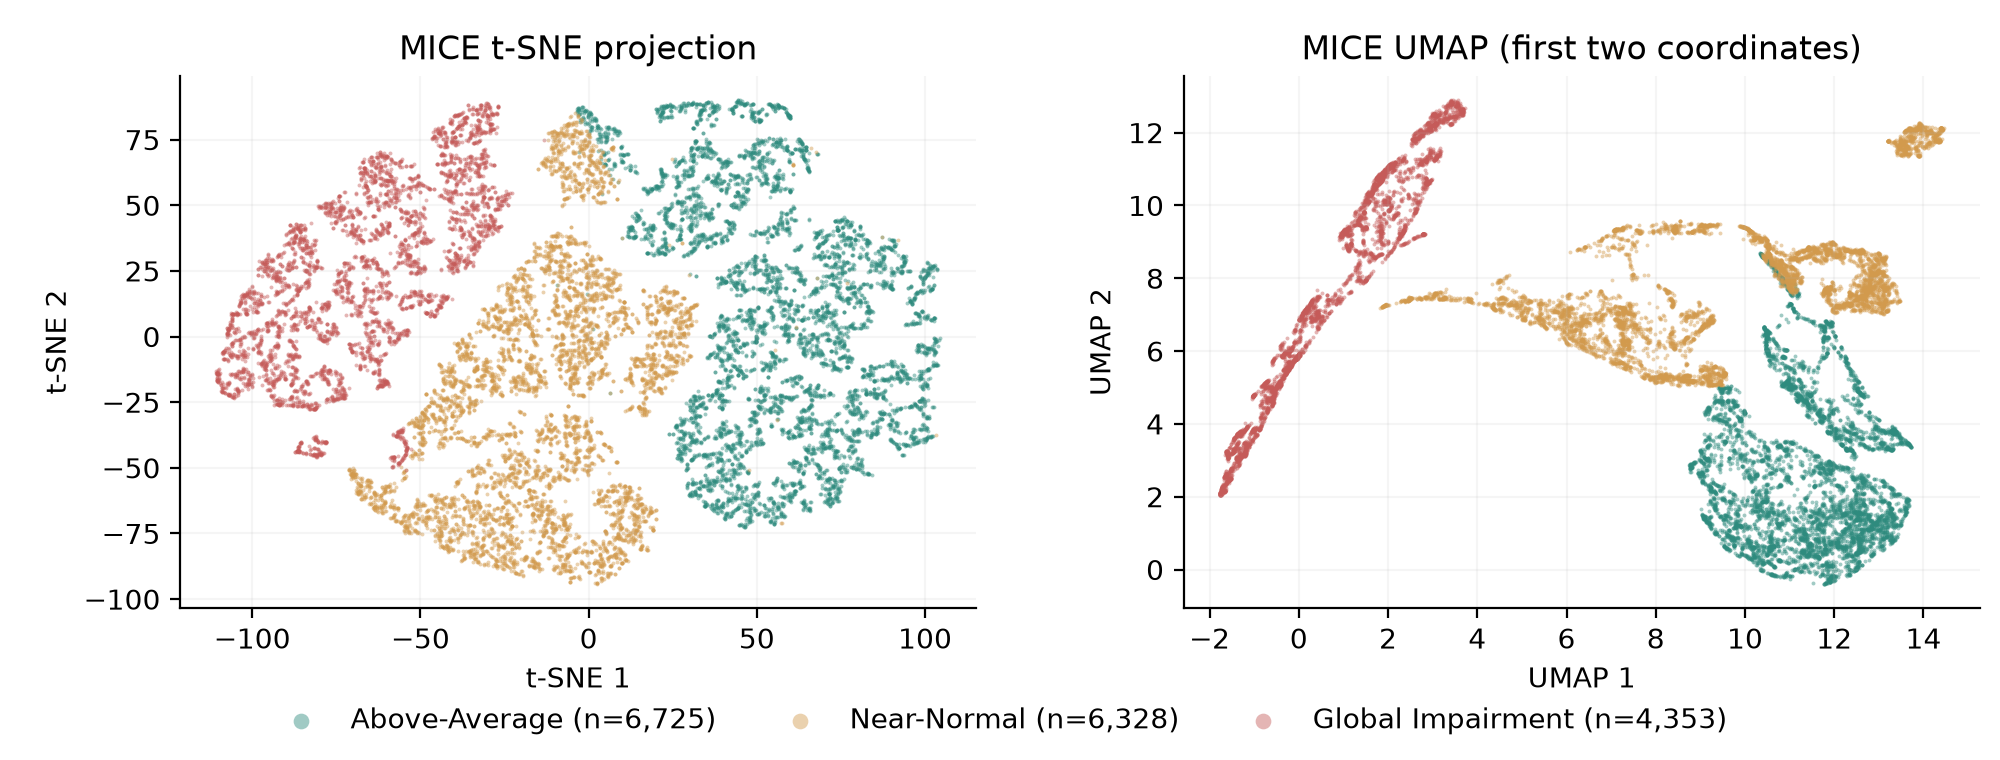
\includegraphics[width=0.9\textwidth]{Figures/tsne_umap_clusters.png}
\captionof{figure}[t-SNE and UMAP cluster projections]{The same 17,406 MICE assessment assignments shown in t-SNE coordinates (left) and the first two UMAP coordinates (right). Colours identify the three final severity bands after noise reassignment; projections illustrate the fitted partition and do not establish discrete phenotypes.}
\label{fig:tsne_umap}
\end{center}

\section{Cognitive Profiles of the Clusters}\label{sec:cluster_profiles}
Below are the radar plots showing mean cognitive domain score per tier, expressed as a z-score from the cohort mean. The three polygons are roughly concentric (every domain moves together), so the tiers differ in overall level rather than in profile shape.



Additionally, I created a random forest surrogate that attempts to recover the tier labels from the domain scores. Gini importance describes each domain's contribution to reproducing those labels. The domains are correlated, and the labels were derived from the same scores. Attention's low importance relative to orientation, visuoperception and language therefore does not establish that attention is clinically unimportant; the ranking is conditional on this fitted partition.

\begin{center}
\centering
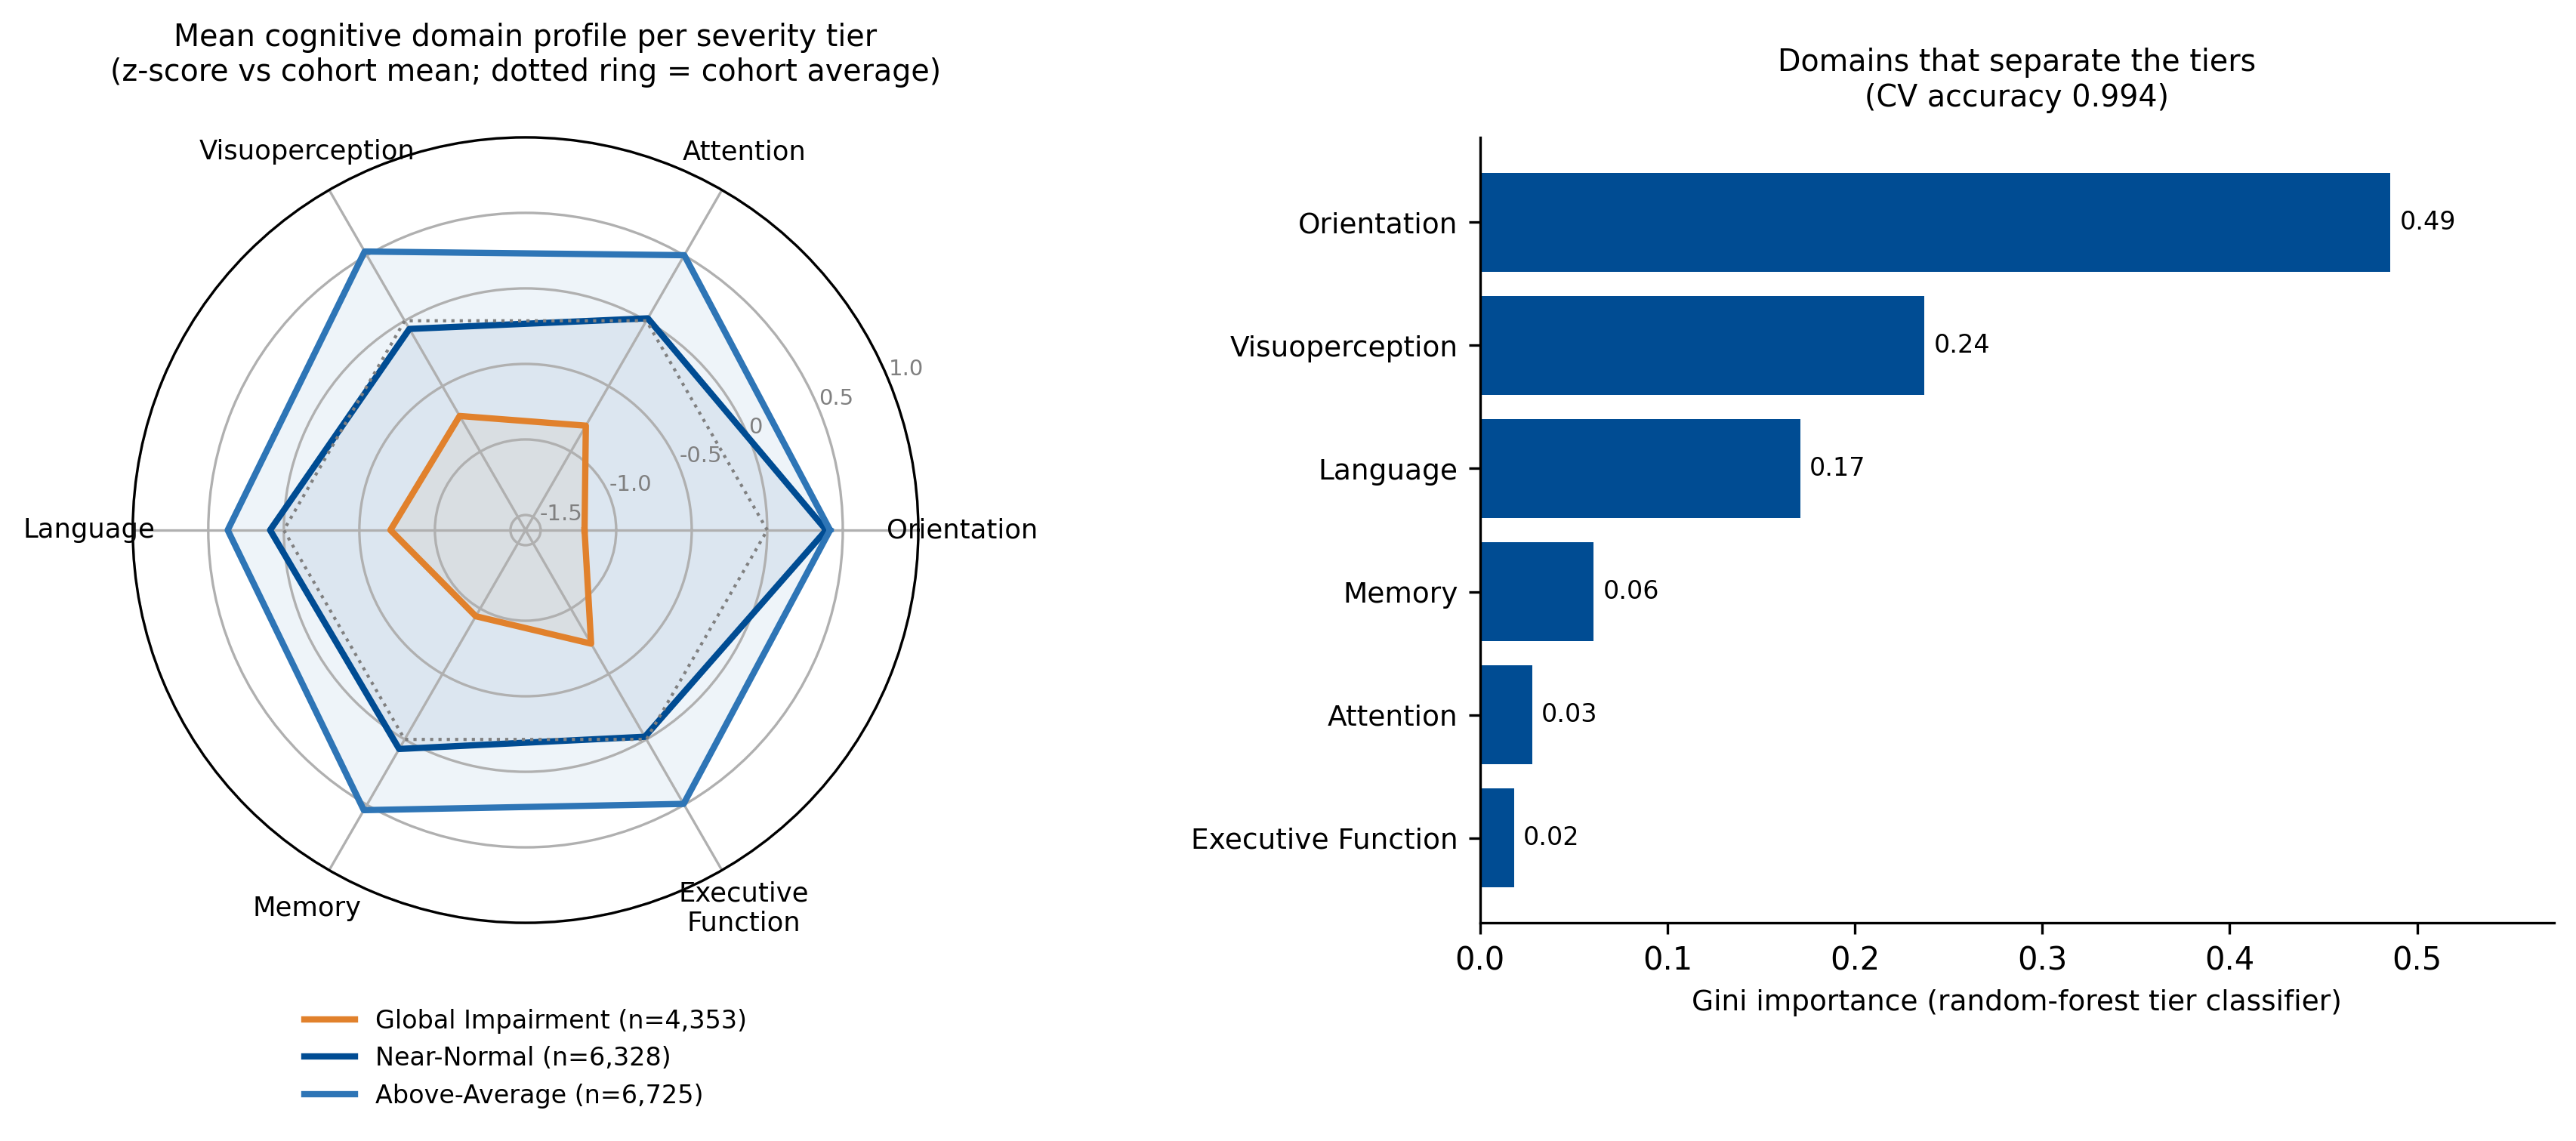
\includegraphics[width=\textwidth]{Figures/cognitive_radar_profiles.png}
\captionof{figure}[Cognitive domain severity profiles]{Left: Mean score for each cognitive domain in each tier, expressed as a z-score from the cohort mean (the dotted ring indicates the cohort average). The three polygons are approximately circular because each domain moves collectively; therefore, the tiers differ in terms of global levels rather than shapes. Right: Gini importance from a random forest surrogate that recovers tier labels from domain scores (accuracy = 0.994). Since these labels are derived from those same scores, this panel describes the decision boundaries of the partitions instead of providing independent importance measurements, and the ordering depends on inter-domain correlation (see Section~\ref{sec:feature_importance}). It should not be interpreted as suggesting that attention has no clinical significance.}
\label{fig:radar_profiles}
\end{center}

\section{Hypothesis 1: Stability and Discreteness}\label{sec:h1_results}
Hypothesis 1 contained two related claims: that reproducible groupings would be recovered and that those groupings would represent discrete cognitive phenotypes. I evaluated stability using 50 bootstrap resamples for each imputation method. HDBSCAN was refitted to each resampled UMAP embedding, and I recorded silhouette, pre-KNN noise proportion, and Hennig core-Jaccard matching. Figure~\ref{fig:h1_bootstrap} shows the bootstrap distributions, while Table~\ref{tab:h1_per_method} reports the exact per-method summaries.

\begin{center}
\centering
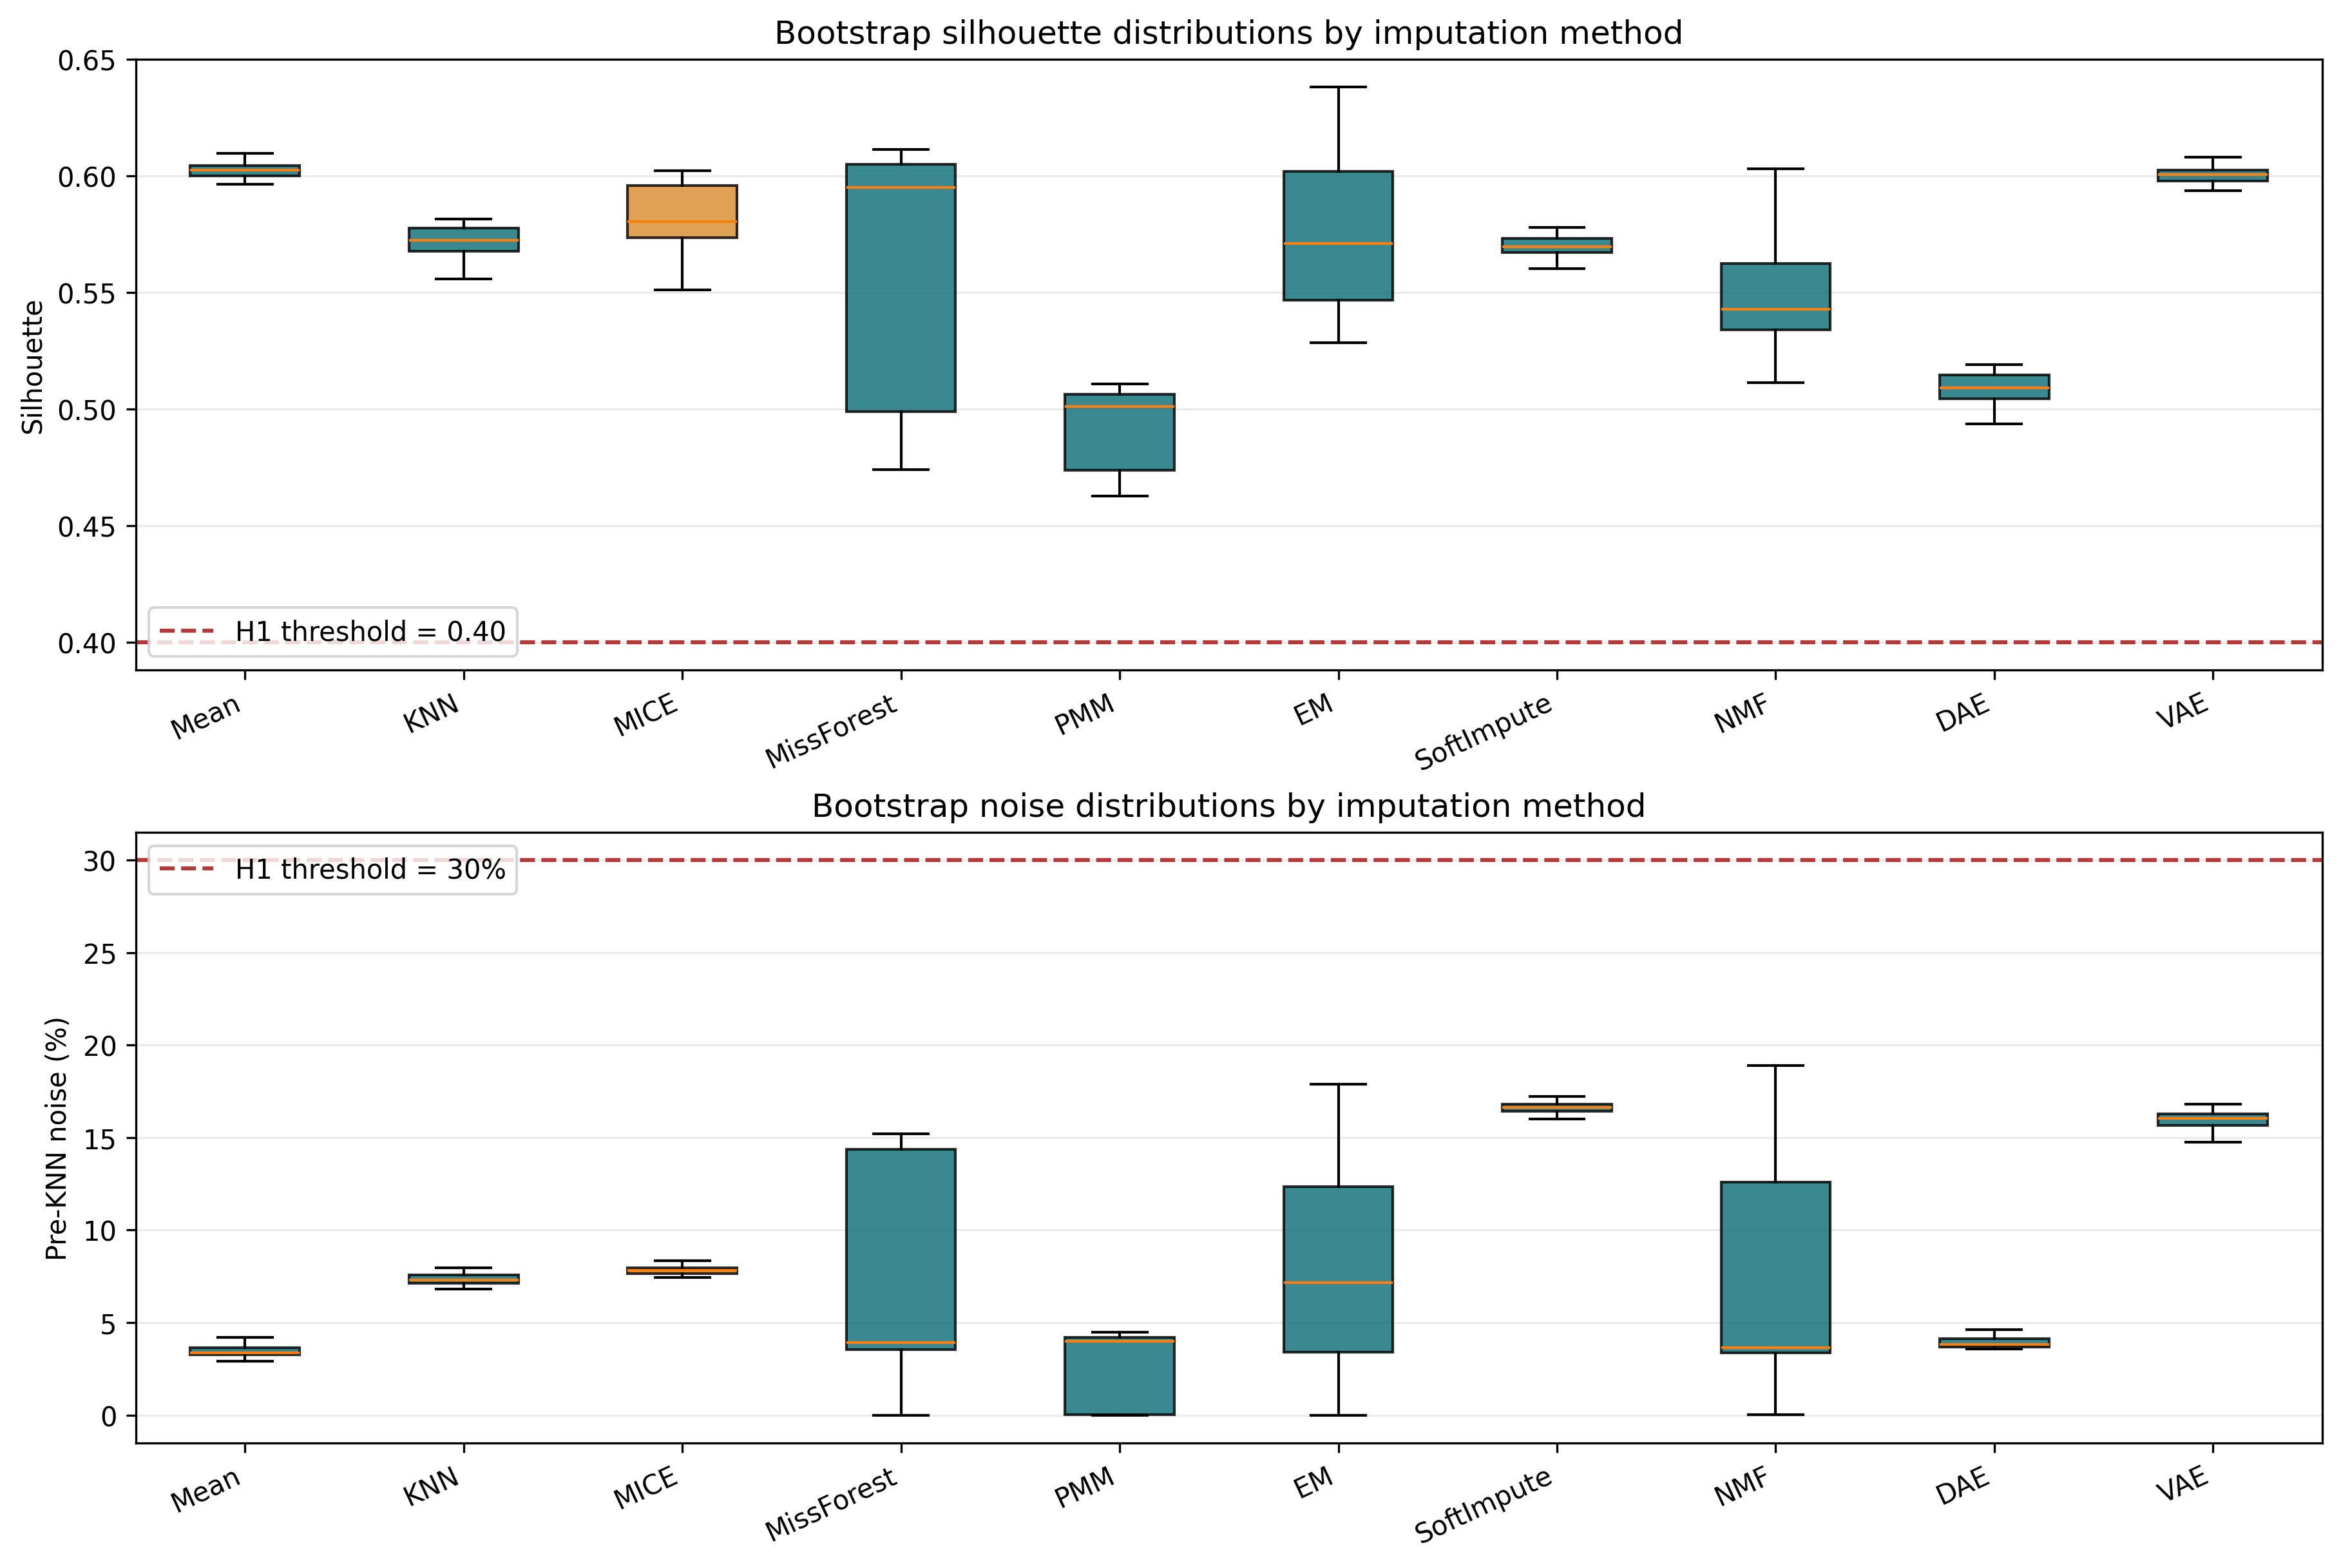
\includegraphics[width=0.92\textwidth]{Figures/h1_bootstrap_distributions.png}
\captionof{figure}[H1 bootstrap stability by imputation method]{Bootstrap distributions of silhouette (top) and pre-KNN HDBSCAN noise proportion (bottom) across 50 assessment-level resamples for each imputation method. Dashed lines mark the pre-specified H1 thresholds. All ten methods met the silhouette and noise criteria, although these values describe stability in the selected UMAP embedding and do not account for repeated assessments within patients.}
\label{fig:h1_bootstrap}
\end{center}

\begin{center}
\small
\captionof{table}[Per-method H1 stability results]{Exact per-method H1 results. Silhouette and noise are bootstrap medians before KNN reassignment. Overall Jaccard is the mean matched-cluster value; the final column gives the range across clusters within each method.}
\label{tab:h1_per_method}
\begin{tabular}{lrrrrr}
\toprule
\textbf{Method} & \textbf{$k$} & \textbf{Silhouette} & \textbf{Noise \%} & \textbf{Jaccard} & \textbf{Cluster range} \\
\midrule
Mean       & 4 & 0.602 &  3.4 & 0.630 & 0.627--0.633 \\
KNN        & 4 & 0.572 &  7.3 & 0.600 & 0.543--0.632 \\
MICE       & 3 & 0.581 &  7.8 & 0.573 & 0.467--0.630 \\
MissForest & 3 & 0.595 &  3.9 & 0.570 & 0.536--0.631 \\
PMM        & 4 & 0.501 &  4.0 & 0.615 & 0.580--0.631 \\
EM         & 4 & 0.571 &  7.1 & 0.509 & 0.383--0.630 \\
SoftImpute & 4 & 0.570 & 16.6 & 0.610 & 0.586--0.631 \\
NMF        & 3 & 0.543 &  3.6 & 0.584 & 0.557--0.631 \\
DAE        & 5 & 0.509 &  3.8 & 0.566 & 0.490--0.630 \\
VAE        & 4 & 0.601 & 16.0 & 0.600 & 0.574--0.631 \\
\bottomrule
\end{tabular}
\end{center}

All ten methods passed the pre-specified silhouette and noise thresholds. However, strict per-cluster reproducibility was weaker: overall core Jaccard ranged from 0.509 to 0.630, and individual matched-cluster values ranged from 0.383 to 0.633, below the conventional 0.70 stability threshold in several cases. Recovered cluster count also varied from three to five. For the MICE labels, full-coverage silhouette was 0.526 in the selected UMAP embedding but only 0.079 in the robust-scaled six-domain space. Together with the concentric profiles and dominant first principal component, these results support reproducible severity ordering but not sharply discrete natural classes. I therefore regard H1 as partially supported: stable severity bands exist, whereas discreteness is not established. Because the bootstrap sampled assessments rather than patients, repeated observations may inflate apparent stability and narrow uncertainty estimates.

\section{Hypothesis 2: Imputation Sensitivity Under a Fixed Partition}\label{sec:h2_results}
Hypothesis 2 posits that different imputation methods will produce largely overlapping assignments when applied to the same incomplete data and evaluated within a fixed embedding and partition model.
The primary tiers were discovered with UMAP+HDBSCAN. For this secondary sensitivity analysis, a StandardScaler, UMAP model, and \(k\)-means labelling rule with \(k=3\) were fitted once to the MICE-imputed domain scores. Every other imputed dataset was transformed and labelled through that frozen pipeline, isolating variation in the imputed values. Across the 45 method pairs, mean ARI was 0.710 and median ARI was 0.739 (range 0.509--0.880). Mean consensus confidence was 0.929, and 86.2\% of assessments met the high-confidence definition of at least eight of ten methods agreeing.

H2 is therefore supported within its defined scope: point assignments are robust to imputation under a fixed embedding and partition. It does not follow that independently refitted UMAP+HDBSCAN pipelines recover identical density hierarchies. Full-pipeline solutions vary from \(k=3\) to \(k=5\), while five independently imputed full-pipeline runs vary from \(k=3\) to \(k=7\). This variability is compatible with discretising a continuum, but does not by itself prove that interpretation.

\begin{center}
\centering
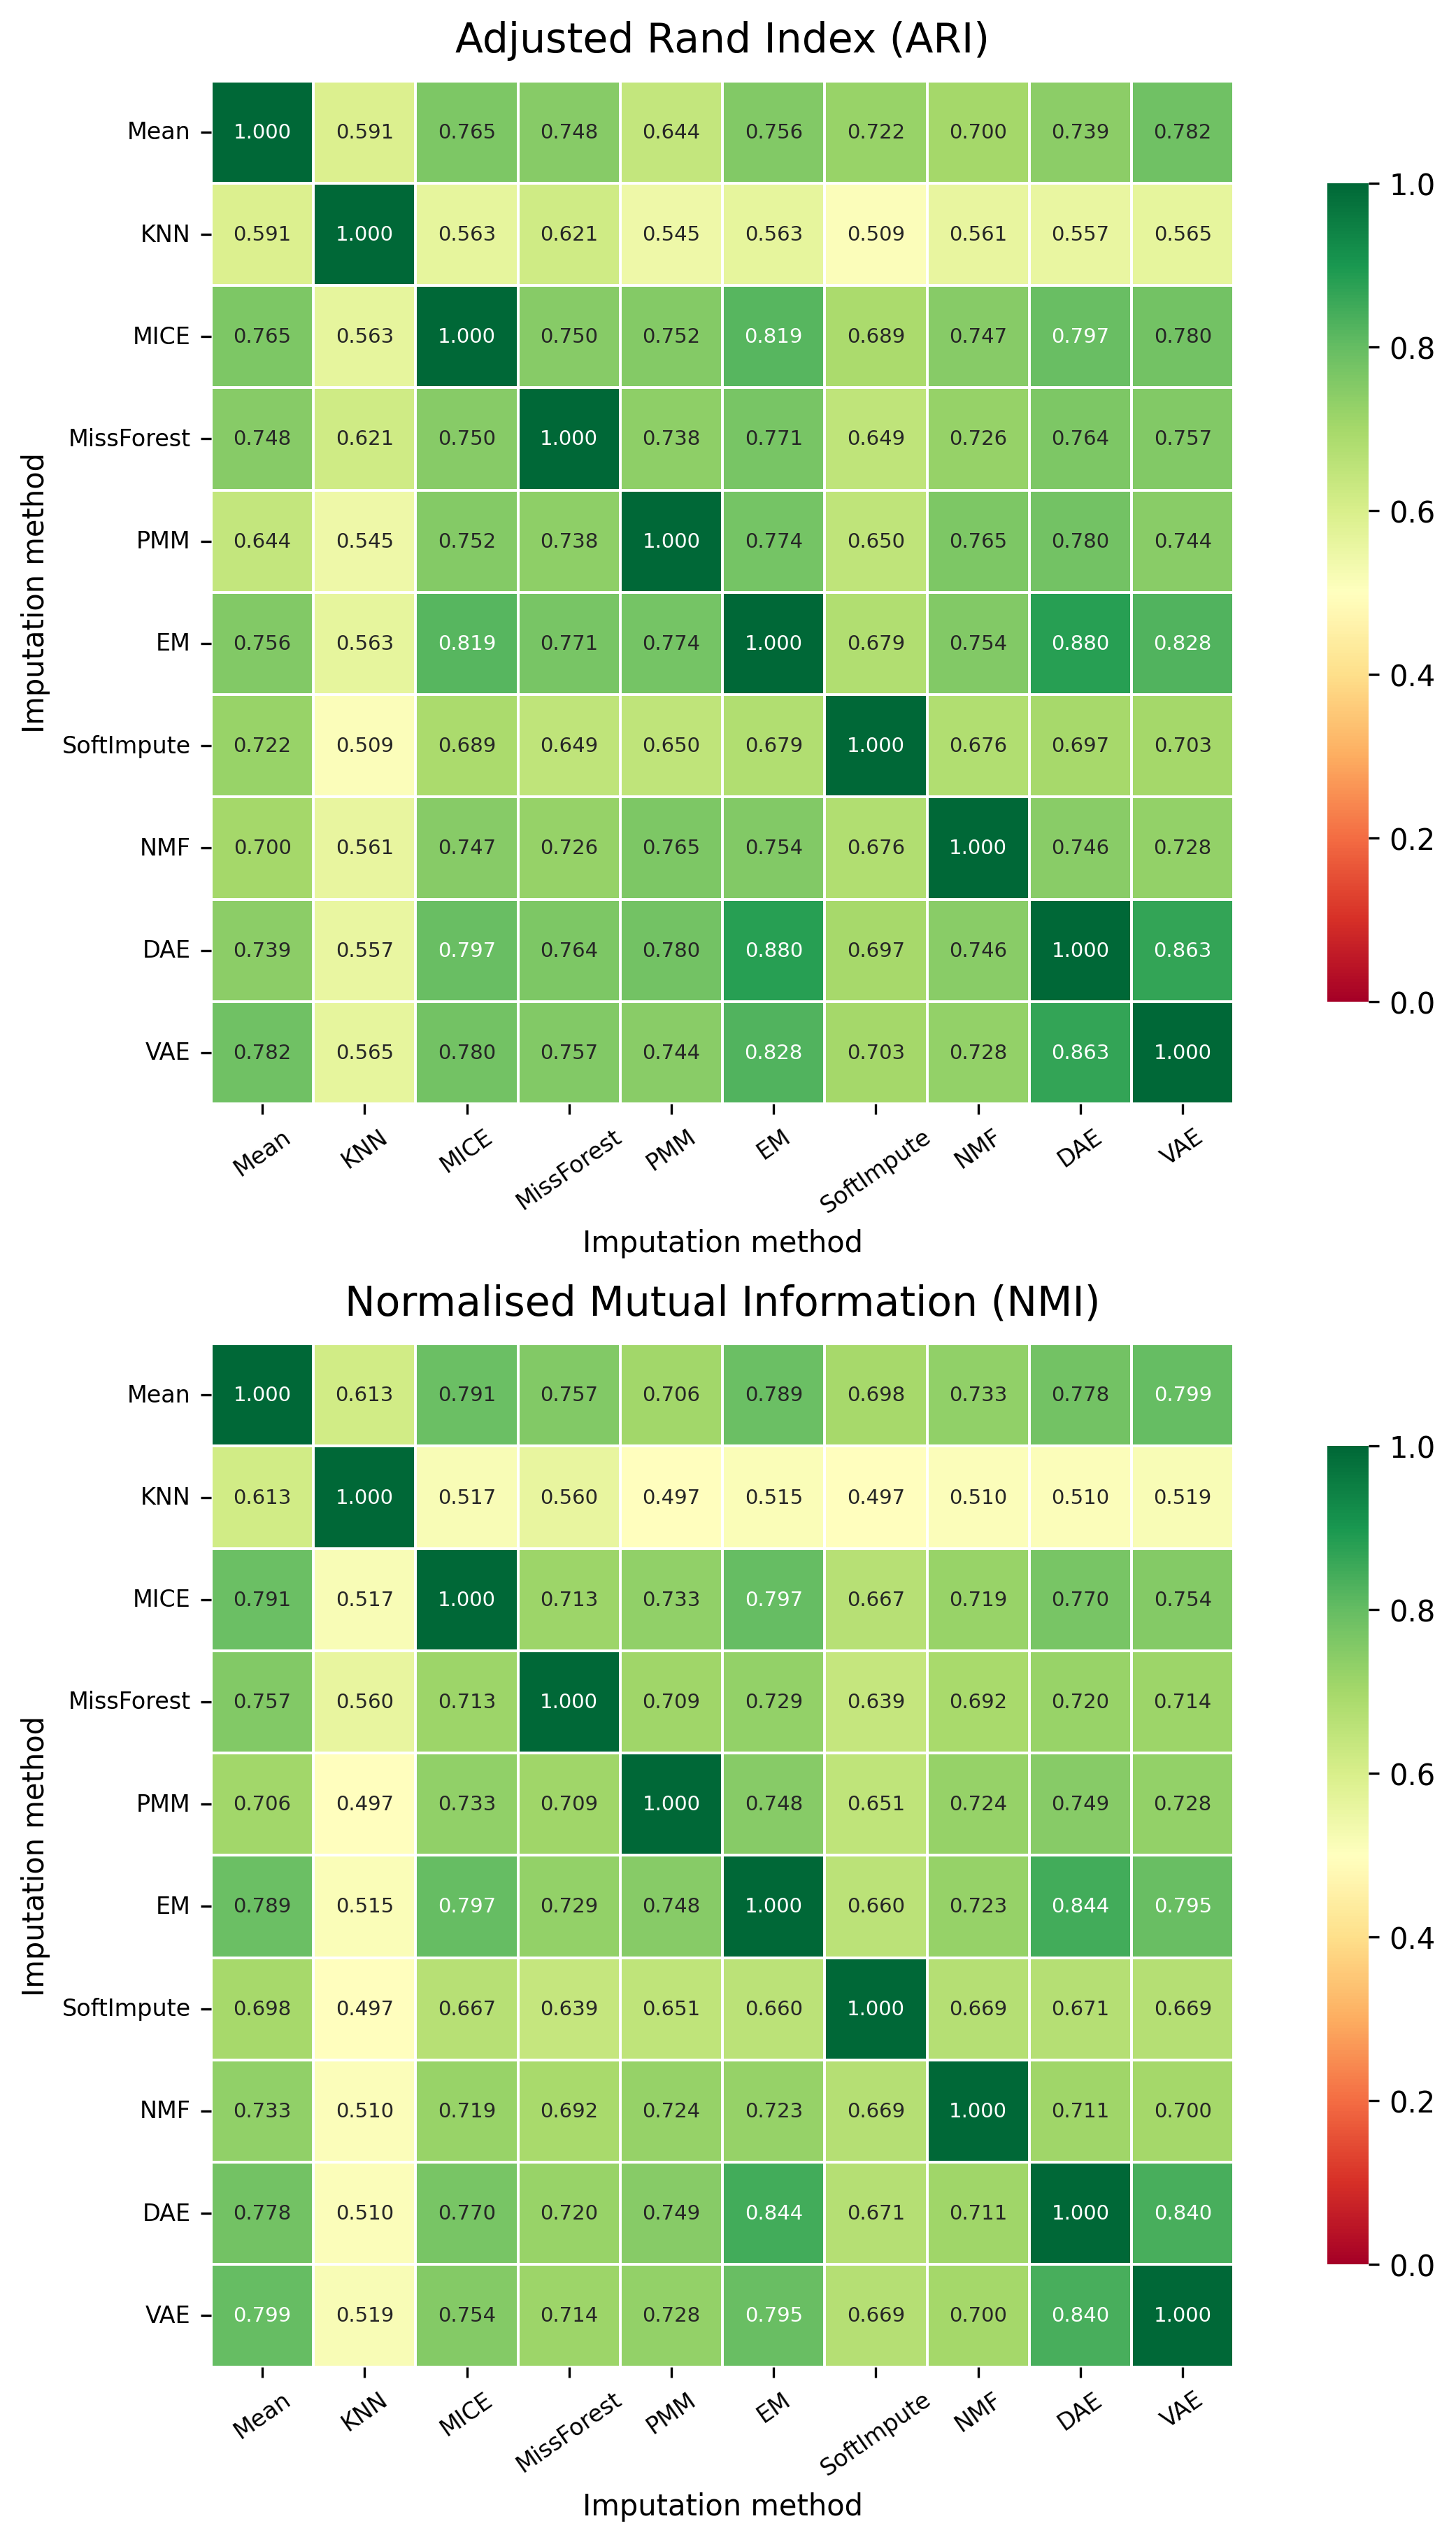
\includegraphics[width=0.88\textwidth]{Figures/h2_ari_nmi_heatmap.png}
\captionof{figure}[ARI and NMI heatmap across imputation methods]{Adjusted Rand Index (ARI) at top and normalised mutual information (NMI) at bottom for pairwise comparisons across the 10 different imputation methods. High agreement was found throughout, although KNN showed lower agreement with the smoother model-based methods.}
\label{fig:h2_ari_nmi}
\end{center}

\begin{center}
\centering
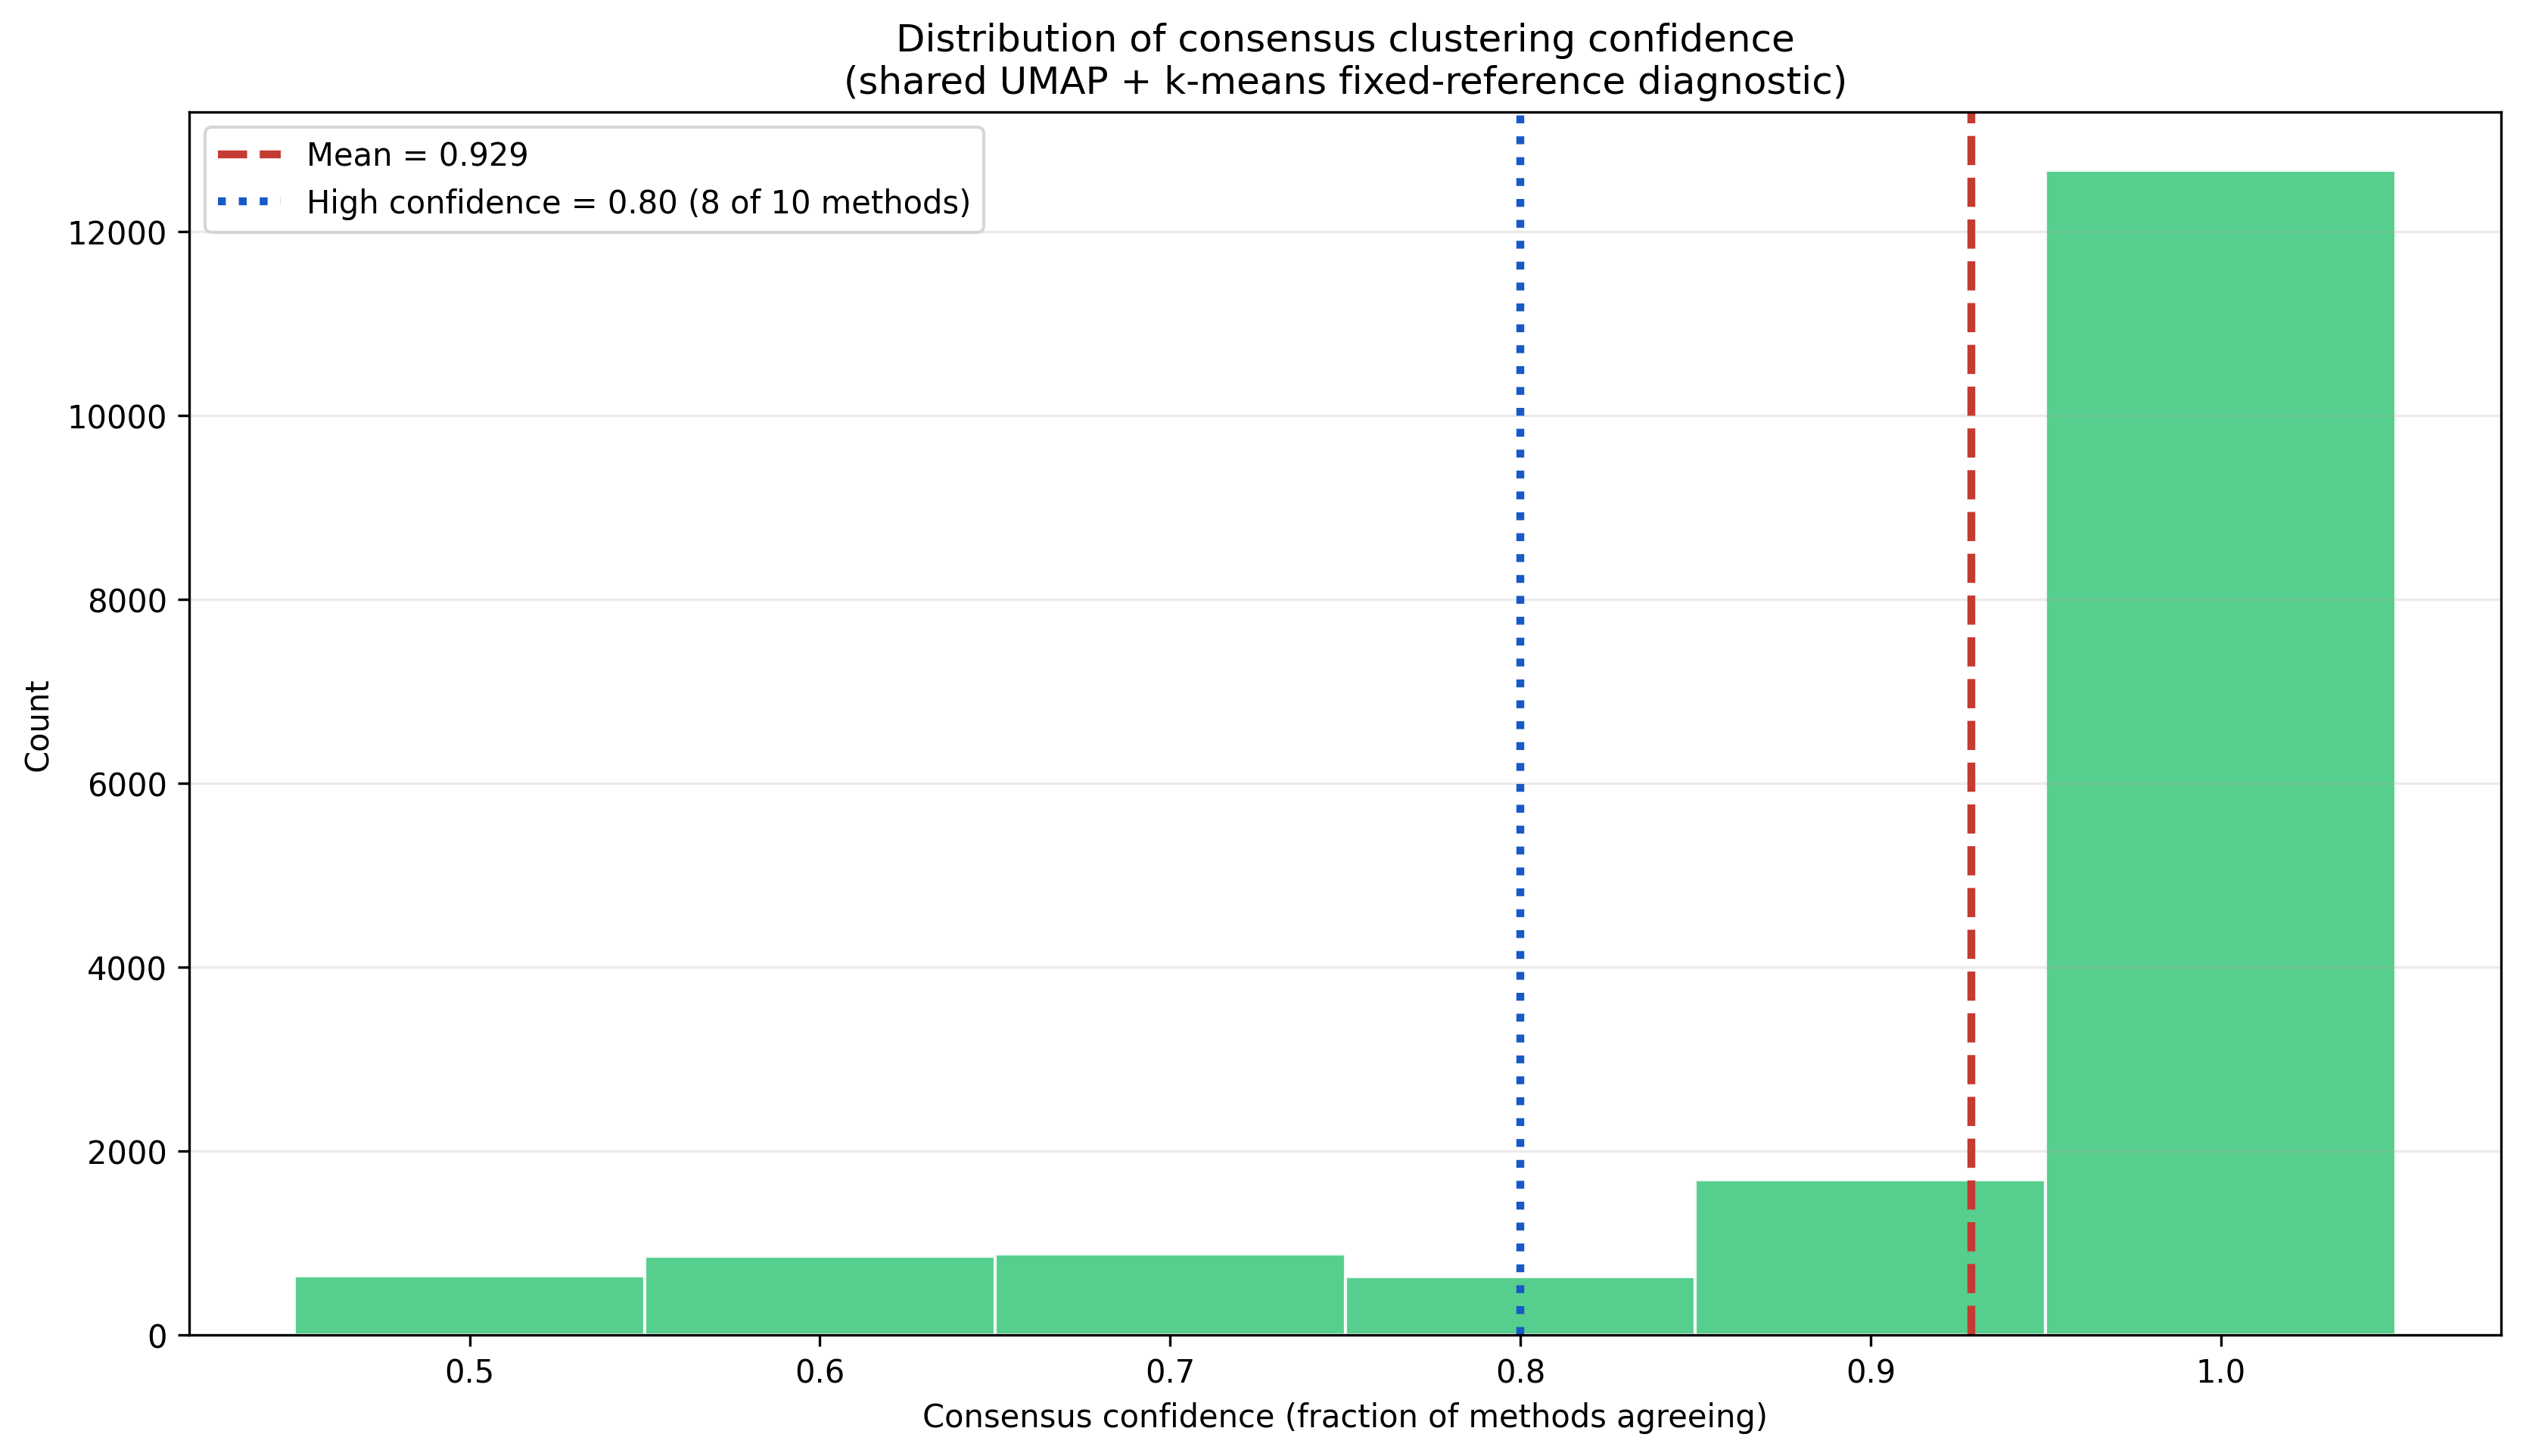
\includegraphics[width=0.85\textwidth]{Figures/h2_consensus_confidence.png}
\captionof{figure}[Consensus clustering confidence]{Histogram of consensus confidence values under the fixed-reference H2 diagnostic. The blue reference line marks the pre-defined high-confidence threshold of 0.80, equivalent to agreement by at least eight of the ten imputation methods. Mean confidence was 0.929, and 86.2\% of assessments met this threshold.}
\label{fig:h2_consensus}
\end{center}

\begin{center}
\centering
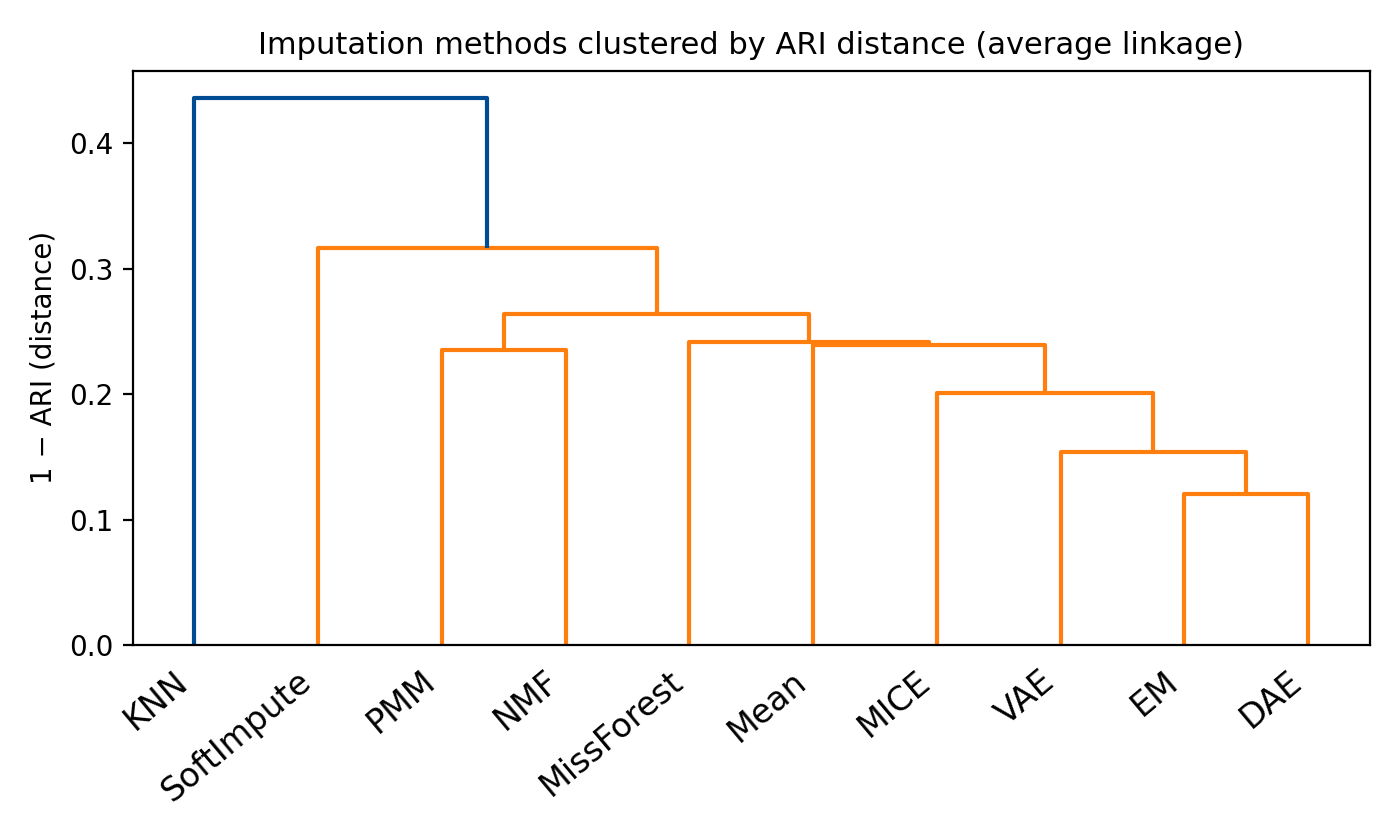
\includegraphics[width=0.85\textwidth]{Figures/h2_method_dendrogram.png}
\captionof{figure}[Method dendrogram based on ARI distance]{Dendrogram of imputation methods using average linkage clustering on ARI-based distance metrics. KNN separates itself from other branches, and tighter grouping occurs among the smoother model-based methods.}
\label{fig:h2_dendrogram}
\end{center}

\section{Hypothesis 3: Clinical Unit Association}\label{sec:h3_results}
Hypothesis 3 tests whether cognitive-severity tier is associated with clinical-unit assignment. The chi-square test showed a statistically significant association ($\chi^2 = 911.3$, $p \approx 4 \times 10^{-156}$), with Cramér's \(V=0.162\). This is a small effect by Cohen's descriptive criteria but exceeds the pre-specified threshold of 0.10. Across five independent MICE imputations, mean Cramér's \(V\) was similar at 0.154; this is an across-imputation sensitivity summary rather than a Rubin-pooled inferential estimate.

A stratified sensitivity analysis indicated that the association remained after accounting for the broad diagnostic grouping supplied by the clinical-unit lookup. Because that grouping is derived from the same lookup as detailed unit assignment, this result should not be interpreted as independent predictive validation.

The patient-grouped multinomial sensitivity analysis provided no clear evidence that tier improved out-of-sample classification of detailed clinical unit beyond the broad diagnostic grouping. Diagnosis-only log loss was 0.6064, compared with 0.6051 after adding tier (improvement 0.0013; 95\% patient-bootstrap CI $[-0.0006,0.0031]$). Accuracy was 0.7772 versus 0.7770, and macro-F1 was 0.476 versus 0.480. I therefore conclude that H3 is supported as an association hypothesis only; the present analyses do not establish added predictive value.

\begin{center}
\centering
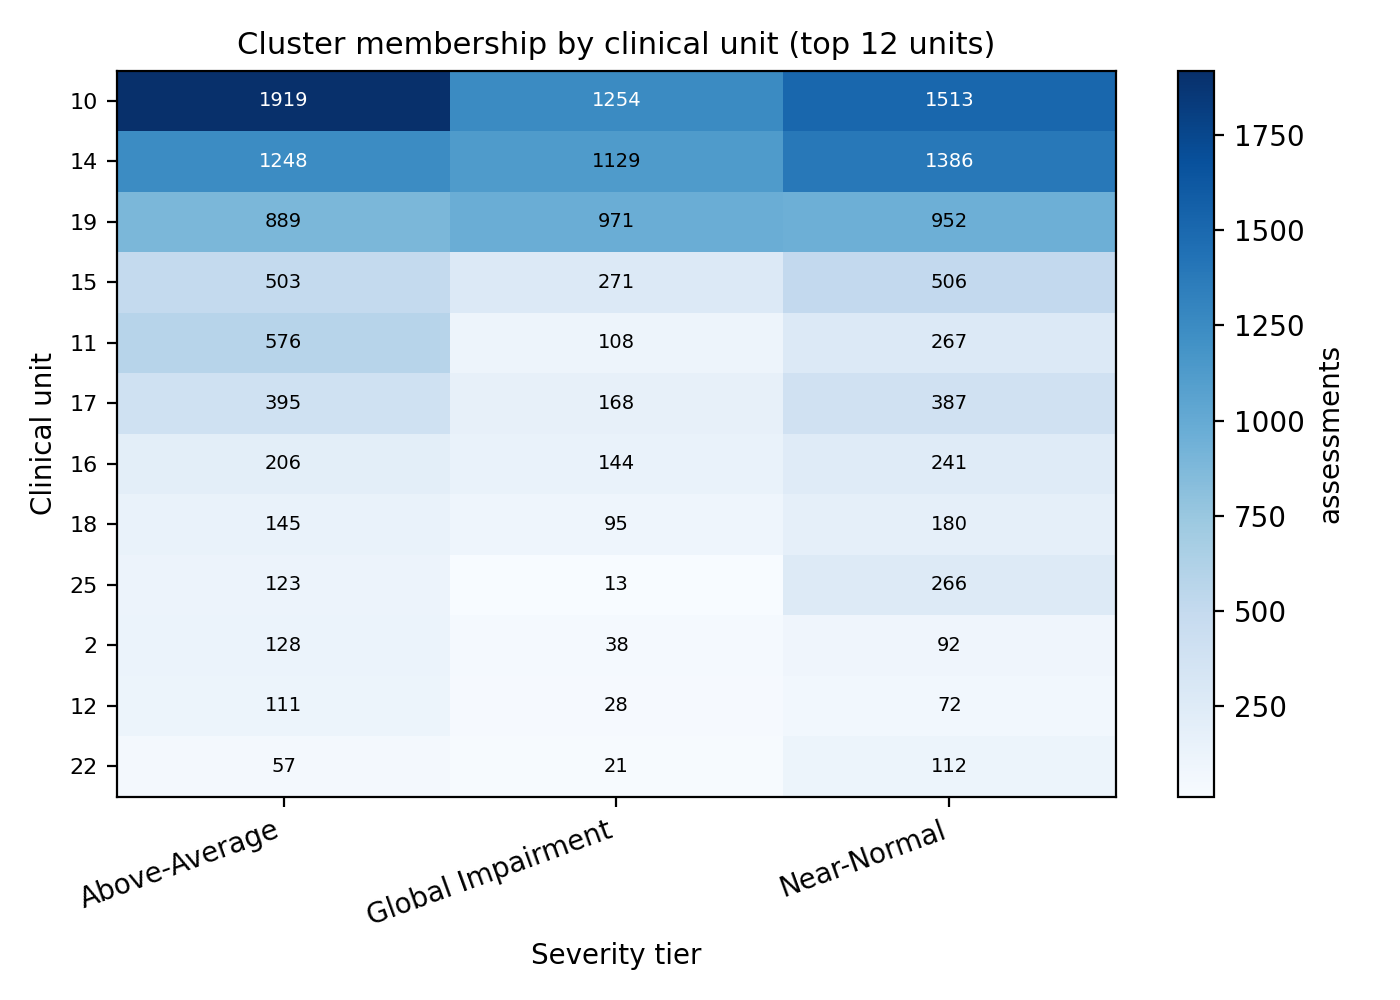
\includegraphics[width=0.9\textwidth]{Figures/h3_clinical_unit_heatmap.png}
\captionof{figure}[Clinical unit by cluster heatmap]{Heatmap of cluster assignments (columns) by clinical unit (rows). Cell colors represent frequencies. Specific tiers occur more frequently in certain units.}
\label{fig:h3_heatmap}
\end{center}

\section{Hypothesis 4: Feature Engineering}\label{sec:h4_results}
The main hypothesis was that domain-aggregate features would reduce redundancy and improve interpretability while retaining separation comparable to the individual variable-level representation. I compared the two representations using silhouette score, condition number, and variance inflation factors (VIFs).



Aggregate measures produced a marginally greater average silhouette score than did the individual variable-based measure (0.481 vs. 0.473; Figure~\ref{fig:h4_comparison}). More importantly, the conditioning of the feature space changed. The average VIF decreased, from 2.77 to 1.88, and the condition number decreased similarly, from 61.7 to 11.8. High VIFs indicate multicollinearity, which distorts computation of distances needed to perform the UMAP and HDBSCAN algorithms. Therefore, the decrease in VIFs indicates that the aggregation process reduced redundancy while maintaining the underlying cognitive constructs measured by the tests \parencite{lezak2012neuropsychological}.



Therefore, Hypothesis 4 is supported primarily through reduced redundancy and improved numerical conditioning and interpretability. The small silhouette difference does not indicate a meaningful increase in cluster separation.

\begin{center}
\centering
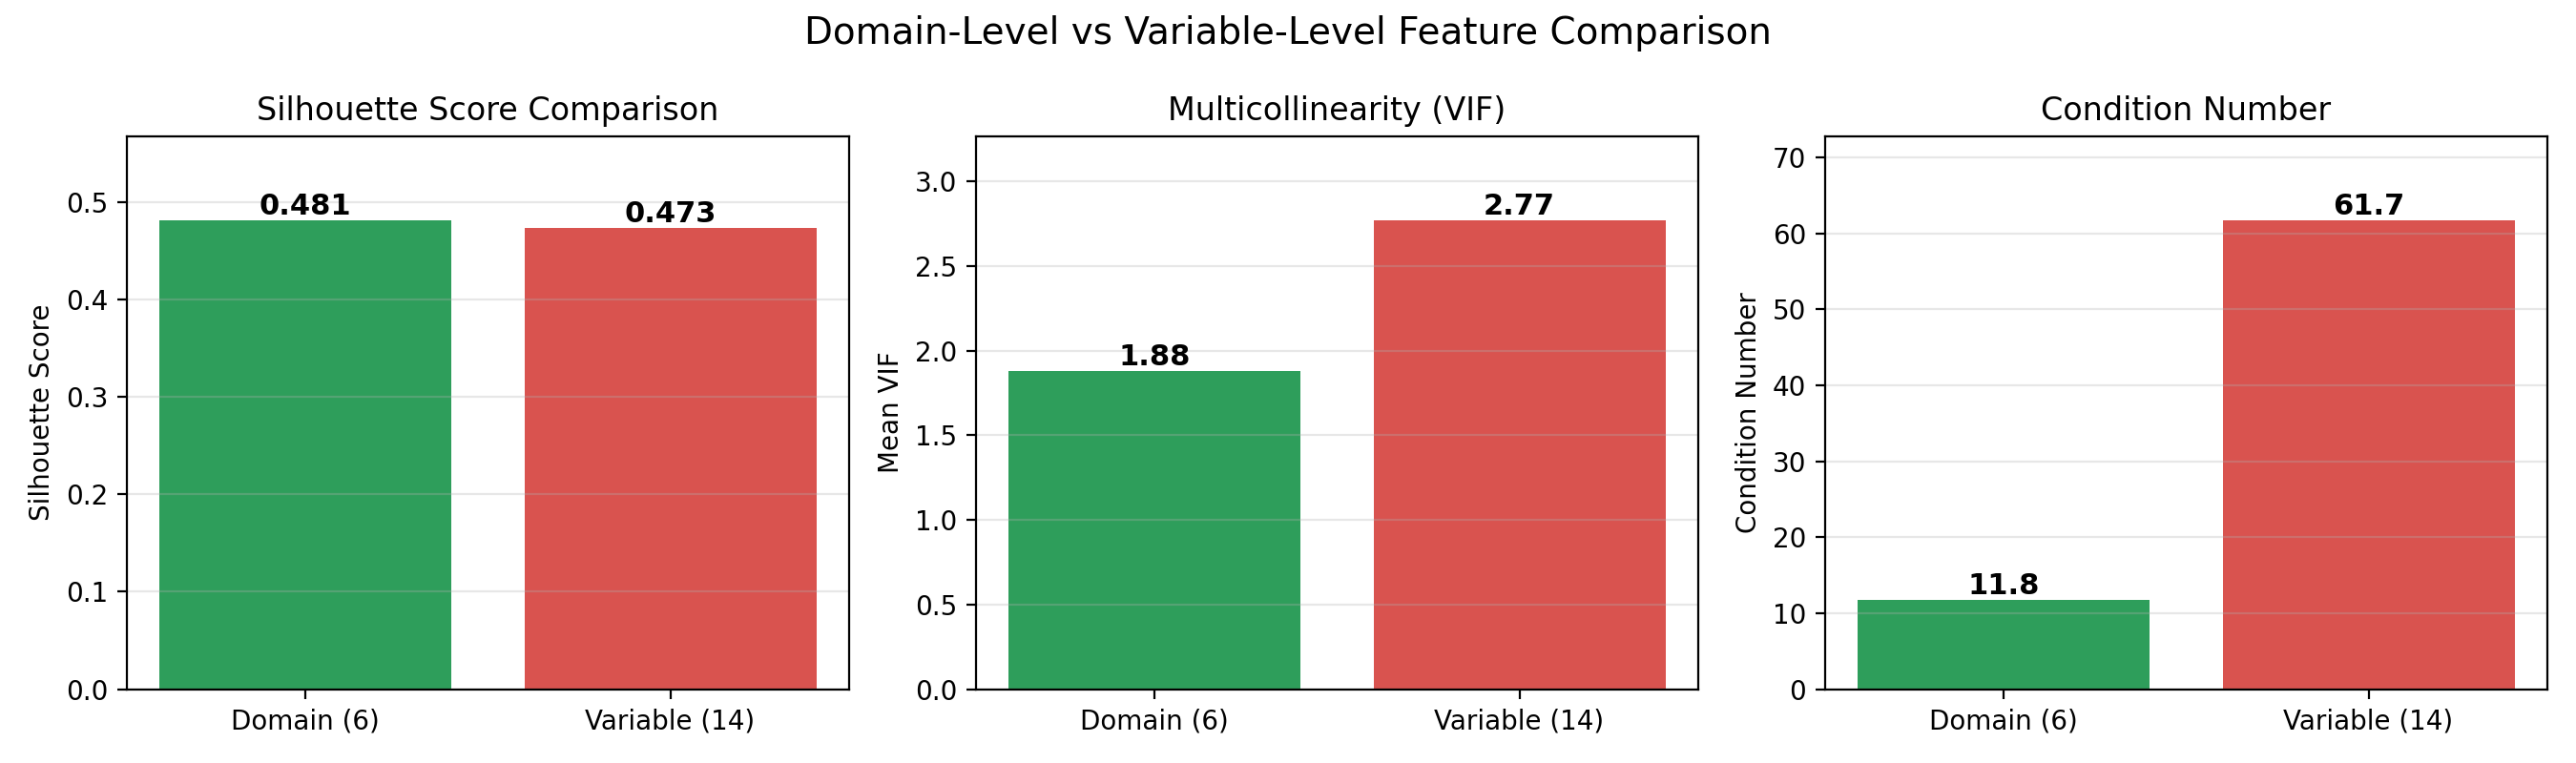
\includegraphics[width=0.95\textwidth]{Figures/h4_domain_vs_variable.png}
\captionof{figure}[Domain vs variable: silhouette, VIF, conditioning]{Comparison of domain-aggregated and variable-level features: silhouette (0.481 vs. 0.473), mean VIF (1.88 vs. 2.77), and condition number (11.8 vs. 61.7). Aggregation at the domain level produces similar separations but much less correlated, well-conditioned features.}
\label{fig:h4_comparison}
\end{center}

\section{Feature Importance Analysis}\label{sec:feature_importance}
I trained a Random Forest surrogate on the MICE-imputed domain scores, using the existing tier labels as targets. It obtained 99.4\% accuracy in five-fold cross-validation. Because those labels were derived from the same scores, this result shows that the fitted partition boundaries can be reproduced. It does not independently establish well-separated natural clusters or predict clinical outcomes.



Gini importance ranked orientation highest (0.486), followed by visuoperception (0.237), language (0.171), memory (0.061), attention (0.028) and executive function (0.018; Figure~\ref{fig:feature_importance}). Permutation importance also placed orientation, visuoperception and language first, but placed attention last. These rankings describe inputs that reproduce the selected labels. Correlated predictors can share or substitute for one another\textquotesingle s contribution, affecting both rankings \parencite{boulesteix2012overview}. A low surrogate importance therefore does not imply clinical irrelevance. The domain profiles and principal-component results in Section~\ref{sec:cluster_profiles} provide complementary descriptions of the severity gradient.

\begin{center}
\centering
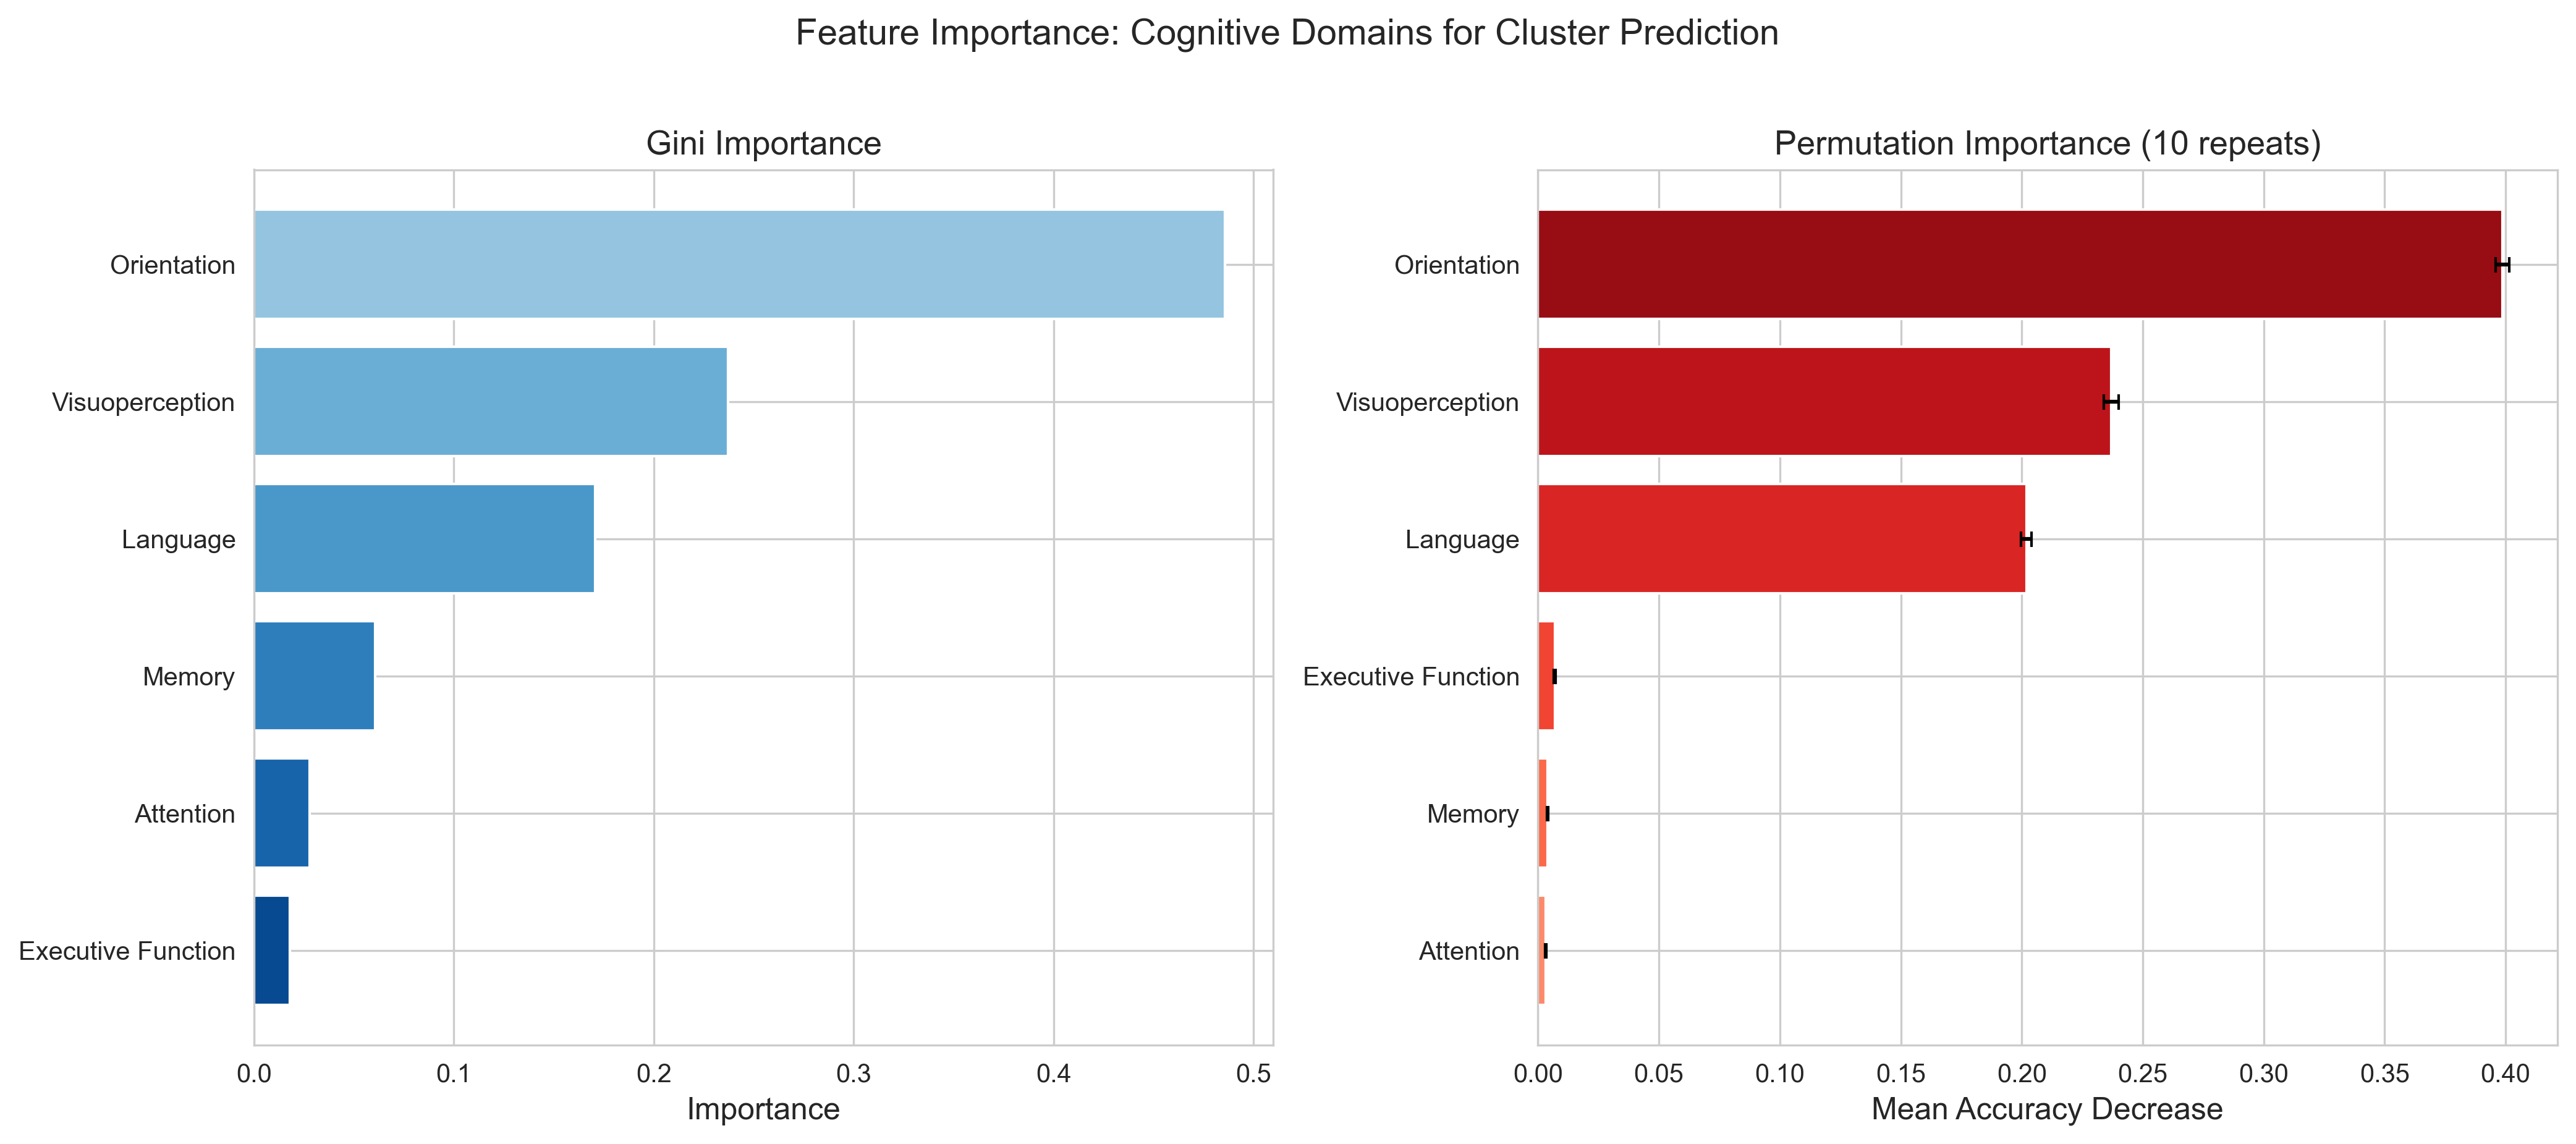
\includegraphics[width=0.9\textwidth]{Figures/feature_importance.png}
\captionof{figure}[Feature importance for cluster prediction]{Random Forest surrogate trained to recover tier labels from domain scores. Left: Gini importance. Right: Permutation importance with error bars. Since labels are derived from the same scores, this panel describes the decision boundaries of the clustering partitions rather than independently evaluating their relative importance. Because the domains are strongly intercorrelated, rankings should not be taken as implying clinical insignificance of attention.}
\label{fig:feature_importance}
\end{center}

\section{Robustness Analyses}\label{sec:robustness}
There are several analyses that help clarify the robustness of the hypotheses. First, I used a "listwise deletion" baseline. Second, I conducted a subsampling stability study. Third, I estimated bootstrap confidence intervals. Fourth, I compared results across independent MICE imputations. Fifth, I described time since injury and within-patient tier transitions. Finally, I used multiple comparison corrections for the 45 pairwise H2 tests.



\textbf{Bootstrap Confidence Intervals.} Assessment-level resampling gives H2 mean ARI 0.710 with a 95\% interval of [0.702, 0.717], H3 Cram\'{e}r\textquotesingle s $V=0.166$ [0.156, 0.175], and an H4 silhouette gap of $-0.002$ [$-0.021$, 0.013]. The H4 interval includes zero and does not support a separation improvement in this supplementary comparison. These saved estimates come from a separate supplementary calculation and need not equal the headline statistics. The earlier raw-test aggregation used in supplementary feature comparisons also differs from the standardized patient-level pipeline. Resampling treats 17{,}406 assessment records as independent, ignoring dependence within 7{,}285 patients; these intervals may therefore be too narrow and should not be interpreted as patient-grouped uncertainty.



\textbf{H2 \& Multiple Comparison Correction.} In order to test H2, I needed to perform 45 different pairwise ARI comparisons against a cutoff of greater than 0.5. Therefore, I applied Holm-Bonferroni corrections to ensure family-wise Type I error rates, and Benjamini-Hochberg corrections to ensure false discovery rates. Using a parametric one-sided bootstrap p-value for each pair, under both types of corrections, the null is rejected for 44 of the 45 pairs; the only exception is KNN-SoftImpute (bootstrap mean \(\mathrm{ARI}=0.509\), 95\% CI [0.497, 0.521]). Thus, with respect to imputation robustness, all method pairs are significant except this one borderline case.



\textbf{Across-Imputation Sensitivity Summary.} I generated \(M = 5\) independent MICE imputations and ran the entire pipeline on each. For each nonlinear statistic, I report the across-imputation mean \(\bar{Q}\) and a descriptive dispersion interval calculated as \(\bar{Q} \pm t_{0.975,4}\sqrt{(1+1/M)B}\), where \(B\) is the sample variance of the five estimates. This calculation uses between-imputation variation only. Because no within-imputation variance was estimated, and because Cramér's V and silhouette are nonlinear statistics, these intervals are not interpreted as Rubin-rule confidence intervals. They are sensitivity summaries showing how results vary across plausible imputations. Mean Cramér's V was 0.154 with a descriptive interval of [0.049, 0.259], and the mean silhouette gap was 0.050 [0.043, 0.058]. The recovered number of clusters varied from 3 to 7, while domain-level features outperformed variable-level features in all five runs.



\textbf{Listwise Deletion Baseline.} If I discard the 46.9\% of the assessments with missing values and apply the pipeline only to the remaining 9{,}245 complete cases, I obtain two clusters with a silhouette of 0.257. Additionally, agreement between the MICE solution for those same assessments and the solution based solely on complete cases is moderate (ARI 0.625, NMI 0.519), yet they are clearly not equivalent. Hence, imputation has a material impact upon the analysis: discarding the 46.9\% of the assessments with missing values changes both the quality and quantity of tiers recovered.



\textbf{Subsampling Stability.} Twenty random 80\% assessment subsamples produce mean pairwise ARI 0.273 and median 0.277. Fifteen fits recover two clusters, three recover three clusters, and two recover no clusters. These results show substantial sensitivity of the historical UMAP+HDBSCAN assignments to resampling. They concern assessment rows and should not be conflated with the separate patient-level k-means stability experiment in Section~\ref{sec:extension_results}.



\textbf{Missingness Threshold Sensitivity.} I also re-ran the entire process -- including variable selection; domain computation; MICE imputation; and UMAP+HDBSCAN -- at five Tier 1 thresholds from 30\% to 70\%. As shown in Figure~\ref{fig:sensitivity}, the solution remains in the two to three tier range with silhouettes ranging from 0.39 to 0.52 over thresholds of 40\% to 70\%. Only at 30\%, where the analysis becomes overly restrictive with regards to how many variables are allowed, does the solution break down. This historical threshold sweep concerns the sensitivity of the selected variables and resulting pipeline. It should not be interpreted as evidence that the main saved matrix applied a 50\% row-missingness limit; the verified row rule is stated in Section~\ref{sec:filtering}.

\begin{center}
\centering
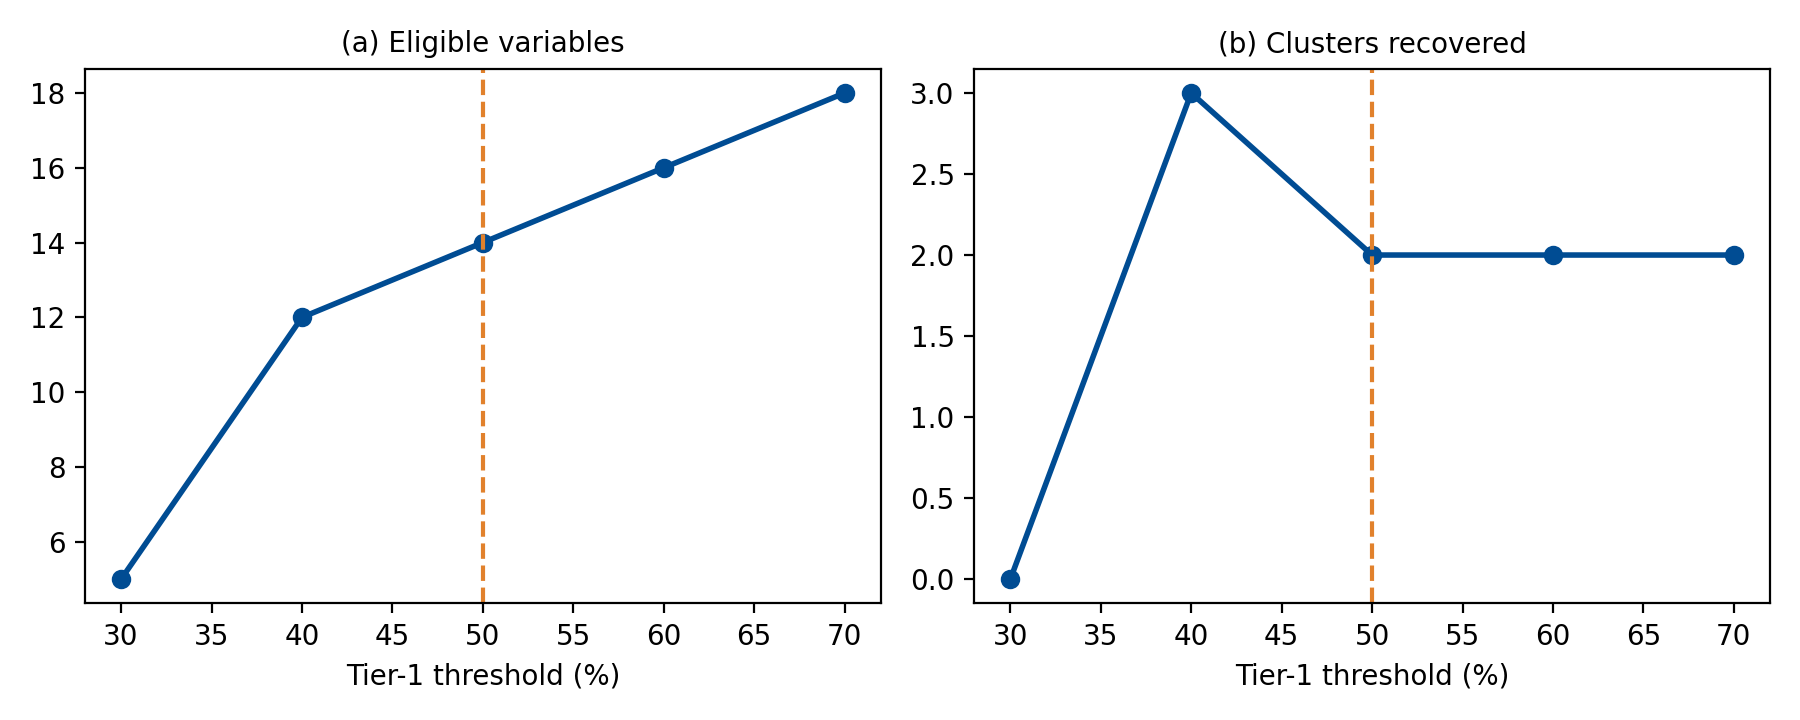
\includegraphics[width=0.8\textwidth]{Figures/sensitivity_analysis_a.png}\\[0.5em]
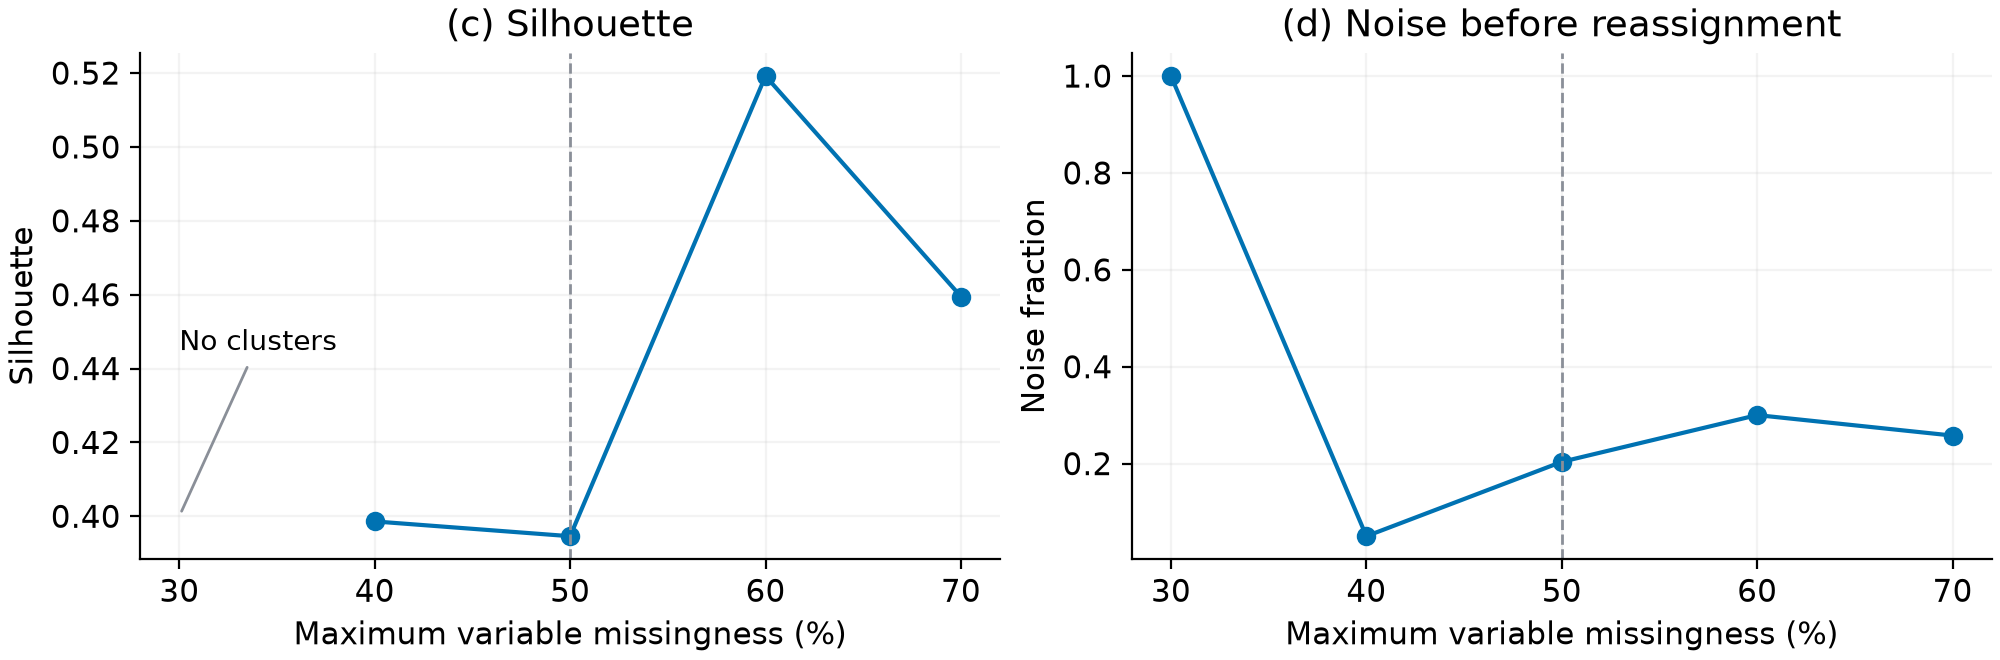
\includegraphics[width=0.8\textwidth]{Figures/sensitivity_analysis_b.png}
\captionof{figure}[Sensitivity to missingness threshold]{Effect of varying Tier~1 missingness threshold across five values (30 -- 70\%). Upper row: (a) Number of available variables and (b) Number of clusters identified. Lower row: (c) Silhouette score and (d) Proportion of noise. The 30\% fit has no clusters, so its undefined silhouette is omitted. Vertical dashed lines indicate Tier~1 missingness threshold used in primary analyses.}
\label{fig:sensitivity}
\end{center}

\textbf{Time Since Injury and Tier Transitions.} Median time since injury is 214 days for Above-Average, 188 days for Near-Normal and 172 days for Global Impairment. These cross-sectional differences do not measure individual recovery or provide an independent functional outcome. Among 5{,}206 patients with repeated assessments, 2{,}613 (50.2\%) remain in the same tier across their observed visits and 2{,}593 (49.8\%) change tier. A subset of 912 patients has exactly two assessments and a tier change: 706 move toward a higher-scoring band and 206 toward a lower-scoring band. This describes movement between cognitive-score bands, not validated functional improvement. Visit timing, discharge and changing test availability may contribute to the observed transitions.



\textbf{Initialization and Resampling.} The historical parameter search repeats UMAP initialization, but seed selection on silhouette is part of model selection rather than independent validation. The saved assessment-subsampling results above quantify a different source of variability. The patient-level extension separately reports initialization and patient-subsampling agreement for its fitted k-means partition.



\textbf{Gaussian Mixture / Latent Profile Baseline.} As a model-based comparison, I fit Gaussian mixture models with full covariance matrices to the imputed domain scores for \(k\) varying from 2 through 6. This analysis is analogous to latent profile analysis in that it estimates model-based continuous-profile classes, but it is not a formal latent profile analysis with full-information maximum likelihood on the incomplete raw data. BIC decreased monotonically with \(k\) (from 243{,}249 at \(k = 2\) to 92{,}606 at \(k = 6\)). This shows only that no BIC optimum was reached within the tested range; it does not establish a continuum, and a solution with more than six components might have been preferred. Mixture-model solutions agreed only modestly with the density-based tiers (\(\mathrm{ARI} = 0.350-0.400\)), while the two-component solution had the clearest silhouette (0.45). I therefore treat this baseline as inconclusive about class number. The continuum interpretation rests primarily on the concentric domain profiles, the dominant first principal component, weak original-space silhouette, and sensitivity of tier count. The observed-data mixture extension in Section~\ref{sec:extension_results} subsequently fits the incomplete test matrix directly, with a wider range of restricted distributional families.



\textbf{Missing-Not-at-Random Sensitivity.} Agreement across imputation methods remains conditional on their assumptions about missing values. The current saved comparisons do not establish robustness to informative test non-completion. A formally specified delta-shift sensitivity analysis, with test direction respected and clinically justified shifts, remains future work.



\textbf{Assessment Eligibility.} Of 22{,}075 records, 17{,}406 had at least one observed value among the 14 retained tests and were eligible for analysis. The remaining 4{,}669 records had no observed values for these tests and were excluded. Absence of retained test values prevents direct assessment of cognitive severity in excluded encounters; it does not establish that their exclusion is clinically innocuous.

\section{Cluster Clinical Naming}\label{sec:cluster_names}
To give the density-based clusters clinically relevant labels, I employed a rule-based naming system based upon the domain-level z-score profiles associated with each cluster.



Clustering profiles associated with domains having z-scores greater than +0.5 were labeled Above Average.



Profiles associated with domains having z-scores less than -0.5 were labeled Global Impairment.



All other profiles were labeled Near Normal.



This resulted in the final labels being Above Average ($n = 6{,}725$), Near Normal ($n = 6{,}328$), and Global Impairment ($n = 4{,}353$).



Since the tiers differ primarily in terms of overall level and not profile shape -- severity labels are preferable to phenotype names.



They provide descriptive shorthand for the historical assessment-level partition. Clinical triage utility has not been established, and these names are not automatically transferred to the new patient-level groups.



CogDash displays the assessment counts and domain profiles for these bands alongside the separate patient-level findings. Group numbers are local to each fitted solution.

\section{Patient-Level Clustering Extension: Results}\label{sec:extension_results}

The new analyses identify repeatable groupings of cognitive scores, while leaving their interpretation as discrete clinical phenotypes unresolved. Results below use the earliest eligible assessment from each of 7{,}285 patients, with 5{,}828 discovery and 1{,}457 validation patients. They are not direct performance comparisons with the historical assessment-level UMAP analysis because the cohort, representation and validation design differ.

\subsection{Original-Space Comparisons and Cluster Count}

Table~\ref{tab:extension_benchmarks} reports representative solutions selected using discovery data. Two-group k-means and PAM were favored in the reference six-domain representation. Direct HDBSCAN assigned all observations to noise under both tested minimum cluster sizes, whereas UMAP+HDBSCAN recovered groups. Increasing UMAP neighborhood size from 15 to 50 changed the recovered count and reduced measured-domain separation. This supports checking embedding-derived partitions in the measured features; it does not rule out other density-model settings.

\begin{table}[htbp]
\centering\small
\caption{Selected patient-level models. Silhouettes are calculated in each row's stated representation; different geometries are not directly comparable. All listed solutions have 100\% validation coverage.}
\label{tab:extension_benchmarks}
\begin{tabular}{p{0.31\textwidth}p{0.22\textwidth}rrr}
\toprule
Model & Representation & $k$ & Discovery & Validation \\
\midrule
K-means & Robust domains & 2 & 0.666 & 0.649 \\
Sampled PAM & Robust domains & 2 & 0.553 & 0.540 \\
Full Gaussian mixture & Robust domains & 8 & 0.117 & 0.118 \\
Tied Gaussian mixture & Robust domains & 5 & 0.548 & 0.535 \\
K-means & PC1 residuals & 3 & 0.547 & 0.532 \\
K-means & 14 tests & 2 & 0.406 & 0.399 \\
UMAP+HDBSCAN & Robust domains & 2 & 0.389 & 0.400 \\
\bottomrule
\end{tabular}
\end{table}

The k-means discovery-silhouette search selected two groups in all 20 stochastic imputations. This is a consistent choice among $k=2,\ldots,8$, not a test against one population. The eight-component full Gaussian domain model also reaches the search limit. Accordingly, neither silhouette selection nor a boundary BIC minimum identifies a unique natural cluster count.

\subsection{Independent Imputation and Patient Stability}

Two- and three-group k-means were highly repeatable conditional on the robust-domain representation and bounded Bayesian imputation model (Table~\ref{tab:extension_stability}). Fixed three-group patient subsampling gave mean pairwise validation ARI 0.968, and varying clustering seeds with the input fixed gave ARI 1.000. Mean matched Jaccard values for the three groups were 0.994, 0.959 and 0.947. These measures describe repeatability within the specified pipeline, not evidence that its groups correspond to distinct clinical entities.

\begin{table}[htbp]
\centering\small
\caption{Pairwise agreement on the same validation patients after independent fits across 20 stochastic imputations. Percentiles describe dependent pairwise comparisons and are not confidence intervals.}
\label{tab:extension_stability}
\begin{tabular}{lrrr}
\toprule
Method & $k$ & Mean ARI & 5th--95th percentiles \\
\midrule
K-means & 2 & 0.959 & 0.944--0.974 \\
K-means & 3 & 0.935 & 0.917--0.951 \\
K-means & 4 & 0.738 & 0.627--0.823 \\
Sampled PAM & 2 & 0.909 & 0.851--0.959 \\
Sampled PAM & 3 & 0.504 & 0.281--0.878 \\
Sampled PAM & 4 & 0.462 & 0.308--0.662 \\
\bottomrule
\end{tabular}
\end{table}

Average-linkage and greedy mean-NMI consensus gave similar agreement for k-means at $k=2$ and $k=3$. Generic NMF aggregation was less reliable: for the two-group k-means ensemble, it reached its iteration limit and collapsed to one assigned group; the requested three-group version produced only two assigned groups. This result concerns ensemble aggregation, not the historical NMF imputation method, and cannot be generalized to all NMF implementations.

\subsection{Scaling, Missingness and Preprocessing Sensitivity}

Robust scaling produced discovery variances of 7.93 for language and 5.76 for orientation, compared with 0.44 for memory. The first component explained 63.3\% of robust-domain variance but loaded predominantly on language and orientation. Narrow central ranges of ceiling-heavy scores amplify their tails under interquartile-range scaling. Equal-domain variance scaling reduced PC1's share to 58.5\% and changed the three-group validation assignments substantially: ARI between the two partitions was only 0.243.

The robust three-group labels had silhouette 0.608 in robust space and 0.440 in equal-domain space. The equal-domain labels had corresponding values 0.172 and 0.283. Figure~\ref{fig:extension_scaling} separates the partition effect from the measurement geometry. Neither geometry is established as clinically correct. Under equal-domain scaling, mean imputation agreement also decreased to 0.769 for two-group k-means and 0.747 for three-group k-means.

\begin{figure}[htbp]
\centering
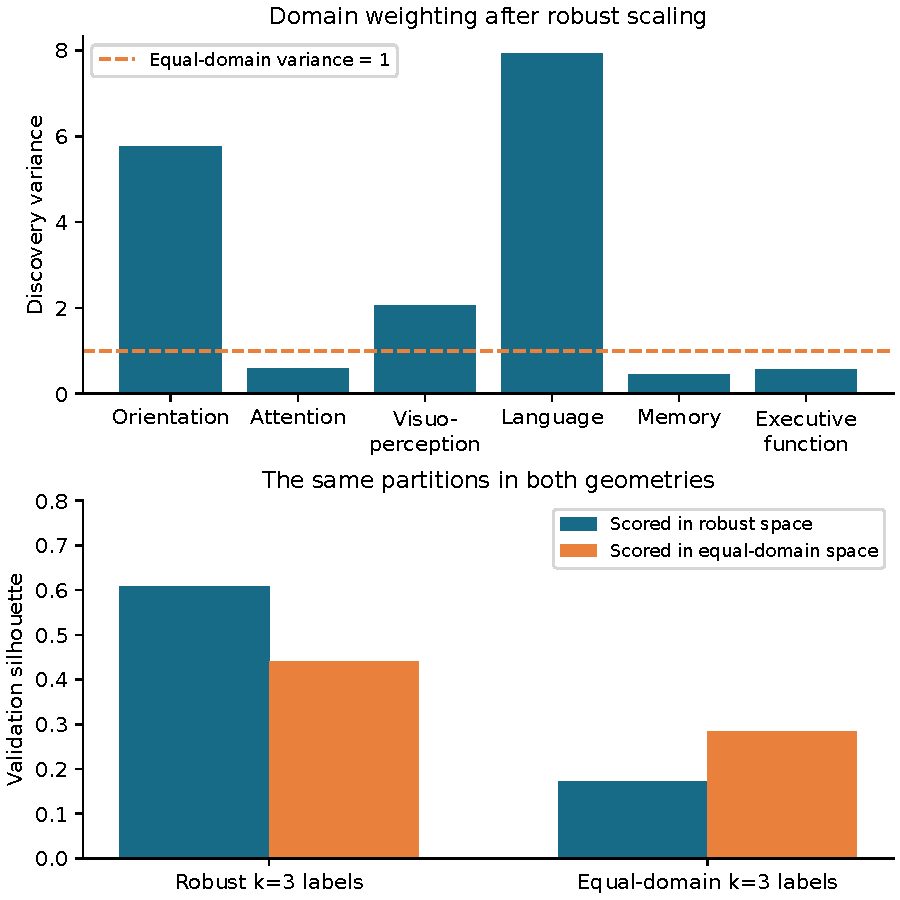
\includegraphics[width=\textwidth]{Figures/extension_scaling_thesis.pdf}
\caption{Scaling sensitivity. Top: domain variances after robust scaling, with unit-variance scaling as a reference. Bottom: the same two three-group partitions evaluated in both geometries. A high silhouette conditional on one geometry does not establish representation-independent subgroups.}
\label{fig:extension_scaling}
\end{figure}

\begin{figure}[htbp]
\centering
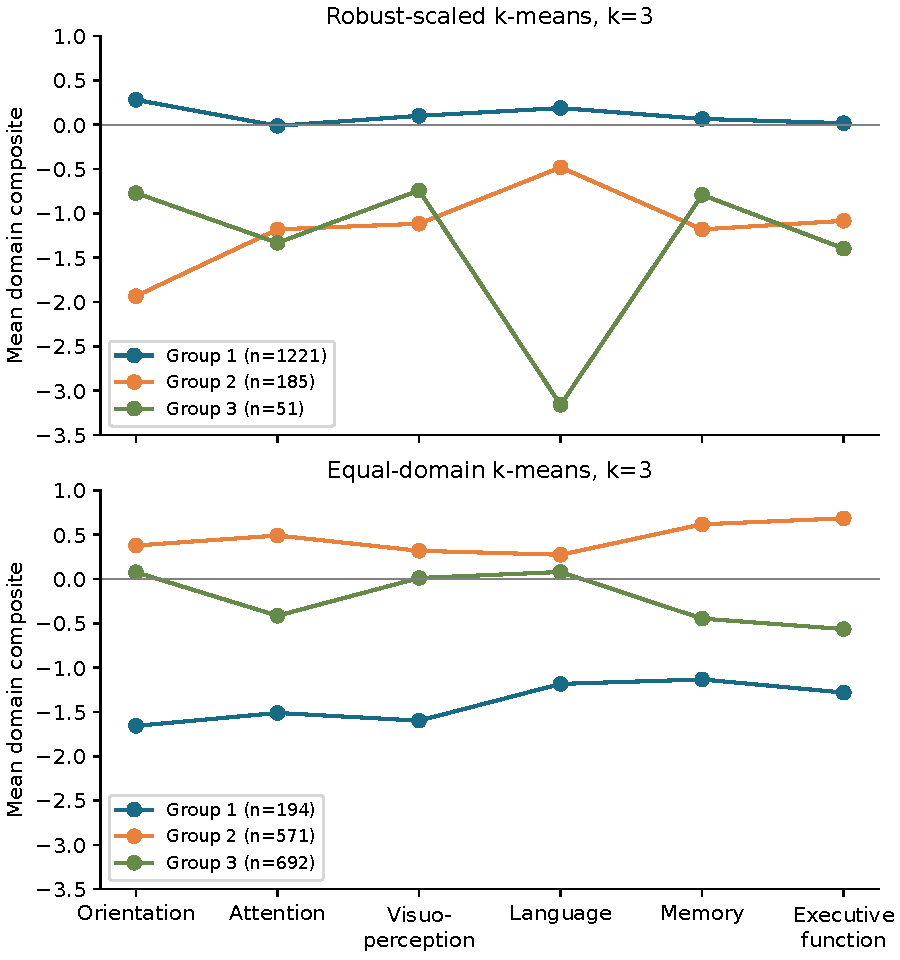
\includegraphics[width=\textwidth]{Figures/extension_profiles_thesis.pdf}
\caption{Validation profiles for fixed three-group k-means under robust and equal-domain scaling. Both panels show the same underlying direction-aligned domain composites. Group numbers and colors are local to each model; matching numbers across panels do not identify the same patients.}
\label{fig:extension_profiles}
\end{figure}

\clearpage
The robust solution contains validation groups of 1{,}221, 185 and 51 patients. Its smallest group shows a pronounced language deficit, whereas equal-domain scaling yields groups of 194, 571 and 692 patients with different profile contrasts (Figure~\ref{fig:extension_profiles}). These exploratory profiles therefore do not justify transferring the historical clinical tier names to the new labels.

Test availability is also associated with the fixed three-group assignments. Cram\'er's $V$ between cluster and missingness was 0.412 for \texttt{MRAVLT075} and 0.371 for \texttt{FEPMR}. Across groups, missingness ranged from 10.2\% to 80.4\% for \texttt{MRAVLT075}, and from 16.1\% to 86.3\% for \texttt{FEPMR}. These descriptive associations do not show that missingness causes the partition, but they prevent interpreting repeatability under one imputation model as freedom from administration effects.

At fixed $k=3$, mean imputation gave ARI 0.921 against the reference assignments, while KNN gave 0.538. Restricting to at least seven observed tests retained 5{,}263 discovery and 1{,}339 validation patients and gave ARI 0.903 on the shared validation subset. Removing clipping gave ARI 0.958. Extending deterministic imputation to 50 iterations converged after 37 and left labels unchanged (ARI 1.000). Independent clustering of validation patients under the frozen discovery transformation gave ARI 0.895; this is an agreement diagnostic rather than another held-out prediction score.

Comparing raw-test aggregation with direction-aligned, standardized domain construction gave three-group ARI 0.703 over all assessments and 0.629 over complete cases. Attention composites correlated $-0.749$ across constructions, highlighting the effect of direction and scale alignment. These descriptive sensitivity checks hold completed values fixed and do not constitute a repetition of the earlier supplementary multiple-imputation and complete-case analyses.

\subsection{Incomplete-Data Mixtures and Continuous References}

Of 32 incomplete-data mixture fits, 28 met the numerical convergence criterion. Table~\ref{tab:extension_mixtures} shows the best BIC fit within each family after the minimum-size and convergence rules. The $t$ family with four degrees of freedom gave the best BIC and validation likelihood among these selected fits. Both $t$ families selected eight components, leaving the optimum unresolved at the upper search limit. Their six-domain silhouettes were low. ICL also selected eight components for both $t$ families, but selected six rather than seven for the contaminated Gaussian.

\begin{table}[htbp]
\centering\small
\caption{Selected observed-data mixtures fitted to 14 incomplete tests. Log likelihood is the mean per validation patient. Silhouette evaluates their assignments in the completed robust six-domain space.}
\label{tab:extension_mixtures}
\begin{tabular}{lrrrr}
\toprule
Family & $k$ & BIC & Validation log likelihood & Silhouette \\
\midrule
Gaussian & 6 & 73{,}878.4 & $-6.076$ & 0.188 \\
Contaminated Gaussian & 7 & 74{,}641.8 & $-6.030$ & 0.154 \\
$t$, df $=10$ & 8 & 69{,}815.8 & $-5.550$ & 0.111 \\
$t$, df $=4$ & 8 & 67{,}545.6 & $-5.341$ & 0.095 \\
\bottomrule
\end{tabular}
\end{table}

These models improve distributional fit without identifying eight validated clinical phenotypes. Multiple components can approximate discrete score masses, skewness and tails. Posterior probabilities quantify membership uncertainty conditional on the selected family and component count, without incorporating uncertainty about model choice or the missingness mechanism.

In the 1{,}000-patient continuous-reference screen, the observed maximum k-means silhouette was 0.676. Its fitted-reference tail fraction was 0.0099, whereas the PC1 dip-statistic tail fraction was 0.9901. The separated positive control recovered two groups with silhouette 0.917. The diagnostics therefore provide different evidence: the silhouette exceeds this particular copula reference, while the projection statistic does not show excess multimodality relative to it. These are descriptive reference comparisons, not an omnibus test establishing clinical phenotypes or excluding all continuous explanations.

\subsection{Longitudinal Findings and Overall Interpretation}

Trajectory eligibility retained 2{,}013 patients: 1{,}590 discovery and 423 validation. All four fitted class counts converged. BIC and validation likelihood improved as classes were added, but every multi-class solution introduced a group below the 5\% expected-membership threshold (Table~\ref{tab:extension_trajectories}). The supplied selection rule therefore retained one trajectory class with continuous patient random effects. Multi-class resampling was not triggered. This is not evidence that all patients recover identically; nonlinear continuous change and small genuine subgroups remain unresolved.

\begin{table}[htbp]
\centering\small
\caption{Patient trajectory models. The 5\% minimum expected discovery-class size is an analysis rule, not a validated clinical threshold.}
\label{tab:extension_trajectories}
\begin{tabular}{rrrr}
\toprule
Classes & BIC & Validation log likelihood & Smallest expected class \\
\midrule
1 & 8{,}376.3 & $-2.598$ & 100.0\% \\
2 & 7{,}572.2 & $-2.403$ & 3.9\% \\
3 & 6{,}806.0 & $-2.290$ & 2.7\% \\
4 & 6{,}465.5 & $-2.212$ & 1.3\% \\
\bottomrule
\end{tabular}
\end{table}

The extension strengthens the evidence that reproducible partitions can be obtained in these cognitive scores. Its principal caution is that repeatability depends on representation and imputation assumptions. Scaling, missingness and distributional family materially affect assignments or component count. Distinct clinical phenotypes remain unconfirmed, and no independent functional outcome was available to establish their utility.


% Chapter 5

\chapter{Discussion}\label{Chapter5}

%----------------------------------------------------------------------------------------
%	SECTION 1
%----------------------------------------------------------------------------------------

\section{Cognitive Structure and the Limits of Phenotype Claims}
The historical analysis recovered broad cognitive-severity structure in this cohort of people with acquired brain injury (ABI), while the patient-level extension recovered reproducible score groupings whose membership depends on scaling and imputation. Together, these analyses do not establish sharply discrete clinical phenotypes or prove that such phenotypes are absent. I identified patients as being in the `above average', `near normal' and `global impairment' tiers based upon their performance across the battery. Importantly, these tiers differ by level, not by profile shape. As illustrated in Figure~\ref{fig:radar_profiles}, each of the six domains moves in the same direction. One principal component explained 56\% of variance in the domain scores and loaded positively across all six domains with similar magnitude. I therefore interpret the result as severity stratification rather than identification of dissociable cognitive profiles. The tiers were associated with clinical-unit placement (§\ref{sec:h3_results}), but the analysis did not establish added predictive value beyond the broad diagnostic grouping.



Moreover, my results inform a broader question in neuropsychology: whether variability across test batteries is primarily domain-specific or dominated by a general factor. I found that in this routinely collected cohort, the general severity axis accounted for most of the recoverable structure. Secondary domain-specific variation was present; however, I did not find that it determined the clustering. I interpret this pattern as consistent with both clinical experience, where global impairment often separates patients before they are differentiated further through narrow dissociations [e.g., \parencite{maas2017traumatic}], and the positive manifold of inter-test correlations found in neuropsychology \parencite{lezak2012neuropsychological}. Therefore, the phenotyping result I report here is more conservative than suggested by some other accounts. Specifically, when I analyzed the data under imputation-robust, sensitivity-tested conditions, overall severity emerged before specific patterns of profiles. I do not over-read this null result: domain aggregation and density clustering on a manifold dominated by a general factor have limited sensitivity to recover narrow dissociations, including an attention-specific subgroup, if such dissociations are small or orthogonal to the principal severity gradient.



My findings do not refute studies that report multiple dissociable cognitive profiles after brain injury (e.g., \parencite{garcia2020data}). Rather, they qualify their interpretations. Unlike those studies, my pipeline differed in several ways. For example, UMAP+HDBSCAN allows for processing of non-convex structures and low-density noise; the bootstrap analysis provided an evaluation of the replicability of the clusters; and each variable was standardized and winsorized in addition to being direction-aligned before forming aggregates. Each of these steps made a difference. High variance raw measures (i.e., a timed Trail making score) can dominate an unstandardized composite; non-cognitive variables can establish artificial axes; nearly empty records can disrupt density estimates. Thus apparent phenotypes may represent artifacts of preprocessing rather than true neuropsychological structure. Chapter~\ref{Chapter6} will examine this relationship further.



I regard H1 as partially supported (§\ref{sec:h1_results}). All ten imputation methods met the pre-specified silhouette and noise criteria, supporting recovery of ordered severity bands. However, overall core Jaccard ranged from 0.509 to 0.630, individual matched-cluster values ranged from 0.383 to 0.633, and the number of recovered groups varied from three to five. These results do not support sharply discrete, uniformly reproducible phenotypes. Boundary movement can occur without disrupting the underlying severity order.



Therefore, I argue that the three-tier solution developed from the primary MICE pipeline should be viewed as an interpretable discretization of a continuum rather than as evidence of natural kinds. Other clustering techniques produce between 3 and 5 tiers depending on how they are configured. Across-imputation and threshold sensitivity analyses show that cluster counts may vary while severity ordering remains consistent. A continuous summary and clearly labeled descriptive groups are therefore both candidates for further validation; their relative clinical utility has not been tested.

\section{Imputation Sensitivity Under a Fixed Partition}
I regard Hypothesis 2 as the major methodological contribution, but I define its scope deliberately narrowly. I discovered the primary clusters with UMAP+HDBSCAN. For the H2 analysis, I then used a separate fixed-reference diagnostic, fitting \(k\)-means once on the MICE embedding and projecting the other imputation methods into that same structure. Under that diagnostic, point assignments changed very little with regard to imputation methods: on average, the 45 method pairs yielded a mean pairwise ARI \(> 0.70\), with 100\% yielding an ARI \(> 0.50\) (§\ref{sec:h2_results}). Therefore, I interpret the easily recoverable structure as a strong severity gradient, whereas a fragile multi-dimensional profile structure is less readily recovered. This distinction likely explains the robustness while still allowing for method-specific variability \parencite{rubin1987multiple}.



Although the imputation process influenced the number of identified tiers and the quality of those tiers, I found that the location of patients along the severity signal did not appear to depend on a particular imputation strategy. I interpret the broad implication as follows: the fixed-reference diagnostic preserves many assignments across the compared imputations. This claim does not extend unchanged to independent model fitting: the new KNN sensitivity gives ARI 0.538 against the reference three-group partition. I do not take this to mean that missing data can be handled casually. Rather, I argue that researchers should treat missingness systematically and report the method clearly, while clinicians should interpret tier labels as aids to judgement rather than as rules that replace medical training or professional experience.



As depicted in Figure~\ref{fig:h2_dendrogram}, I found a strong separation between two families of imputation methods: smooth, model-based methods (EM, DAE, and VAE) that tend to smooth towards a model based conditional mean; local donor-methods (KNN) that rely on a few local donors to plug in missing values. Although many studies use classification criteria related to whether or not an imputation method uses statistical/machine learning/deep learning families, I found the more salient divide to be between smooth and local.



At the assessment level, I found that instability correlates moderately with the fraction of imputed data (\(r = 0.47\); §\ref{sec:h2_results}). As such, I argue that downstream applications should treat assessments with heavy amounts of missing data differently from assessments that contain almost no missing data. This could be achieved by reporting decreased confidence or by comparing more than one imputation strategy.



I view consensus clustering as a practical means of addressing this issue. The ten imputation strategies align their votes regarding label assignments for individual assessments, and the resulting confidence score estimates agreement among strategies. Overall confidence is high (mean confidence 0.93; 86.2\% of assessments have high confidence). However, as I discussed previously, I interpret the lower-confidence assessments as clinically meaningful rather than merely inconvenient. Most notably, these assessments represent patients who are located near tier boundaries and should prompt caution/re-assessment.



In the literature, MICE is commonly used prior to clustering neuropsychological data. MissForest \parencite{stekhoven2012missforest} is often preferred when non-linear relationships are expected. After applying Holm-Bonferroni correction across the 45 pairs of comparison (see Section~\ref{sec:robustness}), I found that 44 of the 45 pairs reject the null hypothesis that ARI \(\leq 0.50\). Only the KNN-SoftImpute pair remains at or near threshold levels. I interpret the broader result, within the fixed-reference H2 design, as clear: the location of patients along the severity signal does not depend upon a single imputation strategy. The number of density-based tiers remains more sensitive when UMAP+HDBSCAN is refitted independently.



The listwise deletion baseline in Section~\ref{sec:robustness} illustrates sensitivity to the handling of missing data. Restricting analysis to complete cases gives a different number of clusters, a silhouette of 0.257 and ARI 0.625 against the MICE solution for shared assessments. This comparison used raw-test aggregation. The controlled comparisons in the extension confirm sensitivity to direction and scale alignment, so the earlier listwise statistics cannot be interpreted as results of the standardized-domain analysis.

\section{Clinical Unit Association}
To determine whether the severity tiers were associated with clinical-unit assignment, I tested the contingency between tier and unit. The association was statistically significant, although the effect size was small by Cohen's standards. A stratified sensitivity analysis remained significant after accounting for the broad diagnostic grouping supplied by the unit lookup. Because this grouping and detailed unit assignment originate from the same lookup, I do not treat that result as independent validation.



The association is clinically plausible, but it is not evidence of prediction or causation. In the patient-grouped multinomial sensitivity analysis, adding tier to the broad diagnostic grouping changed held-out log loss from 0.6064 to 0.6051, with a patient-bootstrap improvement interval that included zero. Accuracy was unchanged to three decimal places. I therefore interpret H3 only as evidence that tier distributions differ across units. Whether severity tier improves prospective routing or outcome prediction requires independent predictors, patient-grouped validation, and clinical outcomes collected for that purpose.

\section{Feature Engineering}
There are many ways to define cognitive features. Two broad options are variable-level features and aggregate features. Variable-level features treat each individual test separately, whereas aggregate features represent averaged or summed versions of tests that are intended to measure a shared cognitive domain. I tested whether domain-aggregate features would be better conditioned than variable-level features. In this context, better conditioned means lower multicollinearity, indexed by smaller variance inflation factors (VIFs), and a smaller condition number.



The results supported H4. I found that domain-aggregate features were much better conditioned than variable-level features even though separation between clusters increased very little. The silhouette changed only slightly (0.481 vs. 0.473); however, mean VIF decreased from 2.77 to 1.88 and the condition number decreased from 61.7 to 11.8 (see §\ref{sec:h4_results}). I therefore interpret H4 primarily as evidence that aggregation reduces redundant information and produces a more interpretable, better-conditioned representation. It does not provide evidence of materially stronger clustering. This benefit supports the clinical practice of interpreting test batteries by domain rather than test by test \parencite{lezak2012neuropsychological}.



I emphasize one critical requirement for aggregation: preprocessing must occur before aggregation. Variables must be winsorized, direction-aligned, and standardized before they can be averaged into composites. Otherwise, differences in raw scale will produce artifacts. For example, if several memory tests are averaged without standardization, the resulting composite can be dominated by whichever test has the largest range rather than by the intended memory construct. If several highly correlated tests enter into an unstandardized composite, then UMAP and HDBSCAN can exaggerate distance computation using a common cognitive dimension. Aggregation provides one feature per domain, but does not ensure equal influence after further scaling. The patient-level extension shows that robust scaling disproportionately weights language and orientation tails.

\section{Feature Importance and What Drives Severity}
I view the findings presented in §\ref{sec:feature_importance} as descriptive rather than explanatory. The Random Forest surrogate produced 99.4\% accuracy using the same domain scores used to generate the labels. Thus, I interpret the ranking as primarily recovering partition boundaries rather than explanatory structures underlying those partitions. The Random Forest ranked orientation, visuoperceptual abilities, and language above attention and executive function; however, I do not give this ordering strong interpretation because the domains are highly correlated. Gini importance is susceptible to variability under correlated predictors \parencite{boulesteix2012overview}.



I consider the principal component structure more reliable. One component explained 56\% of total variance in overall cognitive severity and loaded positively with similar magnitude across all six domains. I interpret this finding as evidence that severity tiers represent general severity levels rather than domain-specific dissociations or attention-specific patterns within this particular domain-aggregated pipeline. Robustness checks presented in §\ref{sec:robustness}, show substantial assignment variability under assessment subsampling and changes in tier count with variable inclusion thresholds. Data-driven studies examining phenotyping should report preprocessing choices clearly and include sensitivity analyses.

\section{Clinical Implications}
I interpret the current results as consistent with a three-tier cognitive severity stratification system. However, I also identify several limits to this approach. The broad clinical implication is conservative: these tiers may help summarize relative cognitive severity, but they should not be used as stand-alone clinical rules. When patients move through the rehabilitation system, clinicians will continue to rely on medical training, local service knowledge, and professional experience when making placement decisions. At present, I do not think these results justify specific recommendations for direct clinical implementation beyond careful interpretation of cognitive severity and transparent handling of missing data.



Clinicians have long relied on visual inspection of patient distributions to identify unusual cases. I interpret the current results as supporting that practice alongside algorithmic clustering. Many assessments did not fall neatly into sharply separated clusters, and I view the central tier as especially consistent with a boundary region cut from a continuum. Because the majority of patients fall along a broad severity gradient rather than within highly separated natural categories, future tools should help identify difficult-to-cluster or boundary-near assessments rather than forcing every assessment into a definitive phenotype label.



Future researchers studying large datasets with missing cognitive data may benefit from additional diagnostics for clustering difficulty. One simple candidate is the proportion of points with very low silhouette values, for example less than 0.05, reported alongside overall silhouette and stability metrics. This would not replace substantive clinical interpretation, but it could help quantify how many assessments sit near ambiguous regions of the partition.

\section{What the Patient-Level Extension Adds}\label{sec:extension_discussion}

The new experiments answer the practical question of whether repeatable clusters can be obtained: two-group k-means was selected across all 20 imputation screens and its mean validation agreement was 0.959. Three-group k-means was also repeatable under the same representation (ARI 0.935), including patient subsampling. This extends the earlier fixed-reference H2 diagnostic by independently refitting partitions while keeping validation patients fixed. The different cohort and feature construction prevent interpreting the larger ARI as an improvement over the historical value of 0.710.

Repeatability and phenotype validity remain different questions. Under equal-domain scaling, the three-group assignments changed substantially (ARI 0.243 against robust scaling), and imputation stability decreased. Missing memory and executive tests were concentrated in some groups. A partition can therefore be highly reproducible while also reflecting the score geometry and administration process. The strong language contrast in one robust-space group is a useful descriptive finding, but its clinical interpretation requires testing under alternative measurement and missingness models.

The likelihood results give a complementary answer. The restricted $t$ mixtures fit the incomplete observations better than the selected Gaussian alternatives, yet both favored eight components at the search boundary. This supports their value as distributional models, without identifying an optimal number of patient types. Similarly, improving trajectory likelihood with additional classes did not produce a solution satisfying the specified minimum-class-size rule. Neither result demonstrates the absence of small subgroups.

These findings fit the questions raised by recent incomplete-data, ensemble and longitudinal research \parencite{tong2025mixturemissing,tomo2026ensemble,julia2026longitudinal}, but the present implementations and cohort differ from those studies. The defensible synthesis is that reproducible cognitive score groupings exist under specified analytical choices, while distinct clinical phenotypes remain unconfirmed. An independent outcome comparison of continuous scores alone versus scores plus group membership, followed by external replication, is needed to establish whether categorical assignments add useful information.

% Chapter 6

\chapter{Limitations and Future Work}\label{Chapter6}

%----------------------------------------------------------------------------------------
%	SECTION 1
%----------------------------------------------------------------------------------------

\section{Limitations}\label{sec:limits}
Firstly, there is only one research site for this study; consequently, every piece of data collected in this study originated from a single rehabilitation unit. This may lead to selection bias which means that the ability to generalize these findings to other clinical populations cannot be confirmed. However, the tests are extensively studied and have international validity, while the six cognitive domains provide a common framework for describing post-injury cognition. Validation across multiple sites is required prior to considering this severity structure to represent ABI broadly instead of representing this specific rehabilitation unit.

Secondly, most historical analyses treated the 17,406 assessments as separate observations rather than grouping them within the 7,285 patients. While it is true that the repeated follow-up assessments of the same patient(s) will always be correlated by definition, neither the primary clustering method nor the assessment level bootstrap accounted for this correlation. Although utilizing each individual assessment allows for preserving the history of recovery status documented in the clinical records at each point in time, utilizing each individual assessment also can potentially create an overestimation of cluster stability along with creating narrower confidence intervals than what exists when assessments are grouped by patient. The patient-grouped multinomial sensitivity analysis directly assesses H3. The new extension adds additional techniques for both discovery and validation at the patient-level including patient subsampling and integrated random effects trajectory estimation. The new extension does not revise the previously calculated uncertainty intervals resulting from the historical assessment-level analysis.

Thirdly, the recovered model's structure imposes restrictions on how we are able to analyze our findings. Although the available historical data suggest that there exists a wide spectrum of possible degrees of severity, the extension demonstrates that while it is possible to establish replicable partitions amongst multiple ways of representing the same data, such partitions remain highly dependent upon which representation was used. Furthermore, it is not possible using the methodologies discussed herein to establish a singular categorical structure. A majority of the cohort exists along a single dimension that represents overall cognitive degree of severity. The fact that PC1 accounted for approximately 56\% of the total variance in the domain scores is evidence of this. The three tiers established through clustering represent a discretized version of this continuum. As such, the tiers should not be viewed as distinct, phenotypic entities with sharply defined boundaries. The actual number of tiers established will likely be influenced by two factors; namely, how one defines the threshold values separating the cluster(s) from one another and what proportion of the data is missing. Assessments that occur near the boundaries of each tier should also be approached with caution. A continuous severity score may be more representative than discrete tiers (Section \ref{sec:future}).

Fourthly, the analytical methodologies have a limited ability to assess the temporal changes that occur post-injury. As previously mentioned, ABI recovery generally occurs very quickly in the initial phase and slowly thereafter \parencite{ponsford2014longitudinal,maas2017traumatic}. Thus, a single evaluation represents a "snapshot" of an injured person's recovery process at a specific time. Many individuals had multiple evaluations in the dataset, allowing researchers to assess if they could detect patterns or trends of change; however, the timing of follow-up evaluations varied greatly as it depended on clinical needs rather than being part of a standardized protocol.

Of the total population of 5,206 patients who had longitudinal data available (Section \ref{sec:robustness}), 50.2\% remained in the same tier throughout all their study visits. The subset of 912 patients who had exactly two assessments and demonstrated a tier change showed a greater percentage of patients demonstrated increases in scores (n=706) compared to decreases (n=206); thus, the results are compatible with recovery, yet tier movement is not a functional outcome. There are additional variables that may impact tier movement including selection, discharge from care, timing of assessments, and availability of tests.

Further longitudinal studies with standardized assessment time frames are needed to address this question.

Another limitation is how missing values were imputed. As noted previously, it has been shown that the MAR assumption cannot be evaluated using only the observed data \parencite{rubin1976inference,little2019statistical}. For example, a patient may have a missing test score because he/she is unable to complete it. Therefore, if there is a Missing Not At Random (MNAR) mechanism for missingness, then the imputation of those missing values could overestimate test performance. Our comparisons do not provide an upper bound on this bias. We are planning to perform a formal sensitivity analysis of a "delta shift" to assess potential violations of our working assumptions regarding missingness.

Structured co-occurrence of missingness is consistent with test-battery protocols, but does not distinguish protocol-driven from outcome-dependent non-completion. Under a fixed MICE-fitted rule, at least 80\% of the ten methods agreed on the assignment for 86.2\% of assessments. This supports conditional assignment robustness, but does not establish ignorable missingness or agreement among independently fitted pipelines.

Assessment eligibility required at least one observed retained test, so records with many missing entries could be included. The higher number of required observations (seven tests) produced an index-patient population of 6,602. The adjusted Rand Index (ARI) value comparing these to the three-group assignments made by comparison on shared validation patients was 0.903. These results suggest some robustness in regards to excluding records based on sparseness; however, the status of the cognitive state of excluded encounters continues to remain uncertain.

The new observed-data mixture model addresses an issue with the previous historical method (impute-then-cluster) by integrating over missing coordinates. This new model continues to have assumptions about missing data (ignorable), utilizes continuous distributions as approximations for discrete and bounded score values, and uses a "dispersion-floor" to prevent singular solution(s). Fthe of the 32 attempts at fitting the models failed to meet the requested level of convergence. Both selected $t$-distribution families reached eight components, the upper end of the search. As such, the exact number of unique classes identified within these mixtures remain unknown. Additionally, I chose not to implement either skew-$t$ or multivariate contaminated longitudinal models.

As such, feature engineering is still applicable. We remove all non-cognitive measures from the dataset. All test directions and scales are aligned. Winsorization is applied prior to creating composite scores through aggregation. Some potential artificial profile differences could arise based upon those decisions. The primary lesson regarding methodology is that unsupervised phenotyping relies heavily on preprocessing. Researchers will need to assess how variables were scaled, what variables were utilized in addition to how the study population was defined when assigning a clinical label to a distinct phenotype discovered using exploratory methods.

The use of HDBSCAN complicates the task of selecting the best approach to solving problems of this nature because, each parameter used in the models must be evaluated based on how sensitive the models are to those parameters. When we evaluate the performance of the model across all methodologies based on the composite metric \(Q\); we are examining \(9\times120\) possible permutations of the parameters. The biasing upward of the measure of separation obtained in the final embedded representation of the data with respect to an unbiased estimate of cluster quality occurs as a result of the incorporation into \(Q\) of both the silhouette value and the selection of the UMAP seed, which was selected at least partially based on the silhouette value. Based on results from PCA, there is evidence to suggest that there is one large factor (cognitive severity) associated with the data. This conclusion is further supported by the finding that 56\% of the total variance can be explained by PC1. It should however also be acknowledged that there is considerable variation in the exact assignments of samples to groups based on how samples are grouped, as evidenced by a sub-sampling mean ARI of 0.273. Thus, these results do not identify a uniquely correct categorical partition.

Available computational resources were another constraint. While the process of executing the UMAP + HDBSCAN procedure fifty times for each methodology was computationally intense; the modularity of the design enabled parallel processing (i.e., the procedures could be run concurrently), thus, although the cost of computer time for a typical consumer-level laptop was very high; it remained at acceptable levels.

Specific limitations existed in validating the extension. Feature selection was based on the historical full cohort. Equal-domain scaling was explored as a sensitivity after inspecting discovery variances. High ARI across bounded Bayesian imputations is contingent upon the imputation model, and it does not address MNAR. Test availability was associated with cluster membership; neither domain-weighting method has been clinically validated. The reference Gaussian copula was constructed using these same data and generates missingness independently of values. Its tail fractions are descriptive: they do not represent a calibrated omnibus test for overall significance. Although a positive control was run separately from the main analysis, this was not a power study, and no calibrated Silverman test was performed. Furthermore, the consensus summaries produced from validation-assignment vectors are not separately validated predictive models.

Finally, prior supplementary analyses comparing complete-case and multiply imputed datasets aggregated raw test values. In contrast, the patient-level extension aligned both the direction and scale of test results before aggregation. Controlled comparisons evaluated sensitivity to this difference; however, they did not recalculate all the previous statistics within the standardized-domain framework. Therefore, those previously calculated statistics cannot be used to validate the patient-level preprocessing pipeline.

\section{Future Directions}\label{sec:future}
Four prospective areas of research are identified based on the results and constraints discussed earlier.

One implication of the cognitive-severity gradients is that continuous indices of cognitive-severity (e.g. produced through PCA, or produced using supervised learning methods on metrics related to functional performance) can potentially provide better representations of patient status and can be used as better summaries of patient status than categorical tiers. Future studies should investigate how well continuous cognitive-severity indices perform relative to tiered classification schemes in terms of predicting prognosis and determining the optimal intensity of rehabilitation required based upon the needs of the individual, while acknowledging that tiered classification may represent an meaningful discrete representation of continuous data as opposed to representing inherent categories.

A second area of expansion would involve developing the linear random-effects mixture model for repeated assessments taken at fixed intervals, thereby allowing investigators to understand longitudinal development of individuals' recovery trajectories. Specifically, the relationship between initial position along the cognitive-severity gradient at assessment and long term outcomes, as well as whether there are different rates of recovery associated with different levels of severity, could be investigated \parencite{ponsford2014longitudinal}. As previously mentioned, the selection of this longitudinal subset of trajectories was based on available visits and length of follow-up. Additionally, many other aspects remain unexamined including non-linear patterns of change, informative dropout, and additional externally derived measures of function. This current analysis has not established the value of these longitudinal subsets for either prognosis or rehabilitation planning.

Thirdly, multi-center validation is required for cognitive-severity stratification to be regarded as a feature of acquired brain injury (ABI) rather than this specific service. Multi-center studies that compare the outcomes from multiple health care systems and populations as well as different methodologies for assessing cognition will provide evidence of whether the one-dimensional cognitive-severity gradient described herein is consistent across populations with varied demographics, test batteries and schedules for assessing cognition \parencite{maas2017traumatic}.

Fourthly, including neuroimaging data will provide evidence of how the degree of cognitive impairment post ABI relates to underlying neurological mechanisms. Researchers will correlate an individual's position on the cognitive-severity gradient with measures of structural and functional imaging to determine if there are any neural substrates associated with global cognitive impairments after ABI. Such information may also provide guidance regarding the development of interventions \parencite{saatman2008classification,maas2017traumatic}.

% Chapter 7
\chapter{Conclusions}\label{Chapter7}

\section{Summary of Key Findings}

This thesis investigates whether neuropsychological test data in acquired brain injury contain reproducible cognitive structure despite incomplete testing. The historical assessment-level analysis and the new patient-level extension support repeatable score groupings under specified analytical choices. They do not establish sharply discrete clinical phenotypes, and they do not prove that meaningful subgroups are absent.

The historical UMAP+HDBSCAN solution describes three severity bands among 17{,}406 assessments: Above Average (38.6\%), Near Normal (36.4\%) and Global Impairment (25.0\%). H1 is partially supported: selected solutions satisfy the embedding-based silhouette and noise criteria, while core Jaccard agreement is moderate and cluster count varies across methods. A dominant principal component and weak original-domain separation support a broad severity interpretation within that representation.

H2 is supported within its fixed-reference design. Applying a common MICE-fitted scaling, UMAP and three-group k-means structure to other imputations gives mean pairwise ARI 0.710. This measures assignment sensitivity under a fixed rule. It does not imply identical independently discovered density hierarchies, and the historical assessment-bootstrap uncertainty ignores patient dependence. The supplementary multiple-imputation and complete-case comparisons used raw-test aggregation, limiting their comparability with the standardized-domain extension.

H3 is supported as an association hypothesis: clinical unit and tier are associated, with Cram\'er's $V=0.162$. Adding tier to the broad diagnostic grouping did not clearly improve patient-grouped validation log loss; the improvement interval included zero. H4 is supported mainly through conditioning: domain aggregation reduced mean VIF from 2.77 to 1.88 and condition number from 61.7 to 11.8, with only a small silhouette difference (0.481 versus 0.473).

\section{Findings from the Patient-Level Extension}

The extension uses 7{,}285 index patients, split into 5{,}828 discovery and 1{,}457 validation patients. Two-group k-means was selected in all 20 stochastic-imputation screens, with mean pairwise validation ARI 0.959. Fixed three-group k-means gave ARI 0.935 across imputations and 0.968 across 50 patient subsamples. Thus, the analysis did find reproducible partitions of the cognitive scores.

The decisive qualification is sensitivity to representation. Changing from robust to equal-domain scaling changed three-group membership substantially (ARI 0.243). Language and orientation dominated variance after robust scaling, and missingness in memory and executive tests was associated with group membership. High repeatability under one preprocessing and imputation model therefore does not establish stable clinical categories.

Restricted robust $t$ mixtures gave better observed-data fit than the selected Gaussian alternatives, but both selected eight components at the search limit. Their weak six-domain separation and unresolved component count do not justify eight phenotype labels. Among 2{,}013 longitudinally eligible patients, extra trajectory classes improved likelihood but introduced groups below the specified 5\% expected-membership threshold. The rule retained a one-class random-effects model, leaving nonlinear variation and small subgroups unresolved.

\section{Methodological Contribution}

The combined workflow separates fixed-reference assignment robustness, independent refitting, patient resampling, feature geometry and observed-data modeling. Shared preprocessing aligns test direction and scale before domain aggregation. Original-space metrics, posterior uncertainty, model convergence, conditional consensus and trajectory eligibility are reported explicitly. Numerical validation supports the computational implementation, while clinical validation remains a separate requirement.

The primary cohort requires at least one observed retained test. A separate sensitivity analysis requiring seven observed tests assesses the effect of excluding sparsely measured profiles. This distinction makes the role of assessment completeness explicit when interpreting cluster stability.

\section{Implications for Research and Clinical Interpretation}

Continuous cognitive summaries and descriptive groups remain candidates for future outcome validation. Current labels should be accompanied by their preprocessing definition and uncertainty, and should not determine treatment intensity or rehabilitation routing. Neither the clinical-unit association nor repeated cognitive scores provide an independent demonstration of treatment utility. CogDash presents both analysis designs for research, with their interpretation limits and saved-model profile comparisons.

The next empirical priorities are to compare continuous scores with scores plus cluster membership on independently measured outcomes, assess sensitivity to informative missingness and administration practices, and replicate the findings across centers and assessment schedules. Nonlinear longitudinal models and adequately measured small subgroups warrant study, without assuming that additional mixture components identify genuine patient types.

\section{Final Remarks}

Reproducible cognitive score groupings were identified in this cohort. Their membership and number depend on scaling, missing-data handling and model family. The evidence supports a broad organization of cognitive performance and useful questions for further subgroup research; distinct clinical phenotypes and their added clinical utility remain unconfirmed.


%----------------------------------------------------------------------------------------
%	BIBLIOGRAPHY
%----------------------------------------------------------------------------------------

\printbibliography[heading=bibintoc]

%----------------------------------------------------------------------------------------
%	THESIS CONTENT - APPENDICES
%----------------------------------------------------------------------------------------

\appendix % Cue to tell LaTeX that the following "chapters" are Appendices

% Include the appendices of the thesis as separate files from the Appendices folder
% Uncomment the lines as you write the Appendices

% Appendix A

\chapter{Imputation Hyperparameters}

\label{AppendixA}

This appendix lists the hyperparameters used for each of the ten imputation methods evaluated in this thesis. Settings followed published defaults where defaults exist; remaining choices were selected by cross-validation or grid search as noted. The methods themselves are described in Chapter~\ref{Chapter3}, §\ref{sec:imputation}.

\begin{table}[ht]
\caption{Hyperparameters for the ten imputation methods.}
\label{tab:imputation_hyperparams}
\centering
\footnotesize
\renewcommand{\arraystretch}{1.2}
\begin{tabular}{@{} l p{10.5cm} @{}}
\toprule
\textbf{Method} & \textbf{Hyperparameters} \\
\midrule
Mean       & Single-pass arithmetic mean per variable. \\
EM         & Multivariate normal model; convergence $10^{-6}$; max 500 iterations. \\
MICE       & Linear regression per variable; 10 iterations; single imputed dataset for clustering. \\
KNN        & $k = 5$; inverse-distance weighting; Euclidean distance. \\
MissForest & 100 trees per forest; up to 10 iterations; variables imputed in order of increasing missingness. \\
PMM        & 5 donors; 10 iterations; implemented within the MICE framework. \\
SoftImpute & Regularisation chosen by cross-validation over 20 log-spaced values from $10^{-3}$ to $10^{2}$; convergence $10^{-5}$; max 200 iterations. \\
NMF        & Rank $r = 5$ selected by grid search over $\{2, 3, 5, 7, 10\}$; multiplicative updates; max 500 iterations. \\
DAE        & Architecture $15 \to 128 \to 64 \to 32 \to 64 \to 128 \to 15$; ReLU + batch normalisation; dropout $(0.5, 0.3)$; corruption rate 20\% with pattern-aware masking; MSE loss on observed entries; Adam optimiser ($\text{lr} = 10^{-3}$); ReduceLROnPlateau + early stopping (patience 20); 5 runs averaged. \\
VAE        & Same layer dimensions as DAE; latent dim 32; loss $= $~MSE~$+$~$\beta$-weighted KL divergence; cyclical annealing with $\beta_{\max} = 0.1$ over 40-epoch cycles; $K = 20$ latent samples averaged for final imputation. \\
\bottomrule
\end{tabular}
\end{table}

% Appendix B

\chapter{List of Abbreviations}

\label{AppendixAbbrev}

The abbreviations and acronyms used throughout this thesis are listed below.

\begin{longtable}{@{}l p{\dimexpr\textwidth-3.2cm\relax}@{}}
\textbf{ABI}        & Acquired Brain Injury \\
\textbf{ANOVA}      & Analysis of Variance \\
\textbf{ARI}        & Adjusted Rand Index (chance-corrected cluster agreement, $-1$ to $+1$) \\
\textbf{BH}         & Benjamini--Hochberg (false-discovery-rate correction) \\
\textbf{BIC}        & Bayesian Information Criterion (model-selection criterion) \\
\textbf{CI}         & Confidence interval (95\% unless otherwise stated) \\
\textbf{CMH}        & Cochran-Mantel-Haenszel (stratified association test) \\
\textbf{DAE}        & Denoising Autoencoder (deep-learning imputation) \\
\textbf{DBSCAN}     & Density-Based Spatial Clustering of Applications with Noise \\
\textbf{ELBO}       & Evidence Lower Bound (VAE training objective) \\
\textbf{EM}         & Expectation--Maximisation (maximum-likelihood imputation) \\
\textbf{FDR}        & False discovery rate (controlled by Benjamini--Hochberg) \\
\textbf{FWER}       & Family-wise error rate (controlled by Holm--Bonferroni) \\
\textbf{GAIN}       & Generative Adversarial Imputation Networks \\
\textbf{GAN}        & Generative Adversarial Network \\
\textbf{GMM}        & Gaussian Mixture Model \\
\textbf{HDBSCAN}    & Hierarchical Density-Based Spatial Clustering of Applications with Noise \\
\textbf{IQR}        & Interquartile Range (spread used by the robust scaler) \\
\textbf{KL}         & Kullback--Leibler (divergence term in the VAE loss) \\
\textbf{KNN}        & K-Nearest Neighbours \\
\textbf{KW}         & Kruskal-Wallis (non-parametric extension of one-way ANOVA) \\
\textbf{MAE}        & Mean Absolute Error \\
\textbf{MAR}        & Missing At Random \\
\textbf{MCAR}       & Missing Completely At Random \\
\textbf{MICE}       & Multiple Imputation by Chained Equations \\
\textbf{MIDA}       & Multiple Imputation using Denoising Autoencoders \\
\textbf{MLE}        & Maximum Likelihood Estimation \\
\textbf{MNAR}       & Missing Not At Random \\
\textbf{MSE}        & Mean Squared Error \\
\textbf{NMF}        & Non-Negative Matrix Factorisation \\
\textbf{NMI}        & Normalised Mutual Information (information-theoretic cluster agreement, $0$ to $1$) \\
\textbf{NN}         & Near-Normal (the middle cognitive severity tier in the MICE solution) \\
\textbf{PCA}        & Principal Component Analysis \\
\textbf{PMM}        & Predictive Mean Matching (semi-parametric imputation, runs inside MICE) \\
\textbf{RAVLT}      & Rey Auditory Verbal Learning Test \\
\textbf{RMSE}       & Root Mean Squared Error \\
\textbf{TBI}        & Traumatic Brain Injury \\
\textbf{TMT}        & Trail Making Test \\
\textbf{TSI}        & Time Since Injury (days at assessment) \\
\textbf{t-SNE}      & t-distributed Stochastic Neighbour Embedding \\
\textbf{UMAP}       & Uniform Manifold Approximation and Projection \\
\textbf{VAE}        & Variational Autoencoder (deep-learning imputation with latent sampling) \\
\textbf{VIF}        & Variance Inflation Factor (multicollinearity diagnostic) \\
\end{longtable}

%\include{Appendices/AppendixC}

%----------------------------------------------------------------------------------------

\end{document}
